%----------------------------------------------------------
% PACKAGES AND THEMES
%----------------------------------------------------------
\documentclass[aspectratio=169,xcolor=dvipsnames,handout]{beamer}

\usetheme{Darmstadt}
\usecolortheme{seahorse}
\setbeamercovered{transparent}
\setbeamertemplate{footline}[frame number]

\usepackage[hangul]{kotex}
\usepackage{hyperref,graphicx, array, adjustbox, makecell}

% other packages
\usepackage{natbib}
\usepackage{float,pstricks,listings,stackengine,xcolor,calligra}
\usepackage{amsmath,amssymb,latexsym}
\usepackage{booktabs,longtable,multicol,multirow,lscape,rotating}
\usepackage{caption,subcaption}
%\newcommand{\source}[1]{\subcaption*{\raggedright 자료: {#1} } }
\usepackage{threeparttable} % Align column caption, table, and notes
\usepackage{adjustbox} % Shrink stuff
%\usepackage{showframe} % Useful for debugging

% defs
\def\cmd#1{\texttt{\color{red}\footnotesize $\backslash$#1}}
\def\env#1{\texttt{\color{blue}\footnotesize #1}}
\definecolor{deepblue}{rgb}{0,0,0.5}
\definecolor{deepred}{rgb}{0.6,0,0}
\definecolor{deepgreen}{rgb}{0,0.5,0}
\definecolor{halfgray}{gray}{0.55}

\lstset{%
    basicstyle=\ttfamily\small,
    keywordstyle=\bfseries\color{deepblue},
    emphstyle=\ttfamily\color{deepred},    % Custom highlighting style
    stringstyle=\color{deepgreen},
    numbers=left,
    numberstyle=\small\color{halfgray},
    rulesepcolor=\color{red!20!green!20!blue!20},
    frame=shadowbox,
}

\hypersetup{unicode=true,colorlinks=true,linkcolor=blue}

% font조정
%\usepackage{fontspec}
%\setmainfont{Times New Roman}
%\setmainhangulfont{NanumGothic}

% 문자열 대체{노사관계론 전용}
\usepackage{newunicodechar}
\newunicodechar{•}{\textperiodcentered}
\newunicodechar{➔}{$\implies$}
\newunicodechar{∴}{$\therefore$}
\newunicodechar{∵}{$\because$}

%----------------------------------------------------------
% TITLE PAGE
%----------------------------------------------------------
\title{한국의 사회동향 2025}
\subtitle{경제 및 소득•지출 분야}
\author{오성재}
\institute[KIHASA]
    {\relax
        제 5회 한국의 사회동향 포럼
    }
\date{2025년 8월 27일}

%----------------------------------------------------------
\begin{document}
%----------------------------------------------------------

\frame{\titlepage}

\begin{frame}{목차}
    \setcounter{tocdepth}{1}
    \tableofcontents
\end{frame}

\section{경제분야}
\subsection{경제성장}
\begin{frame}[<+->]
\frametitle{광복 후 최빈국에서 80년 만에 세계 10위 경제로 도약하다.}
    \begin{figure}
        \centering
        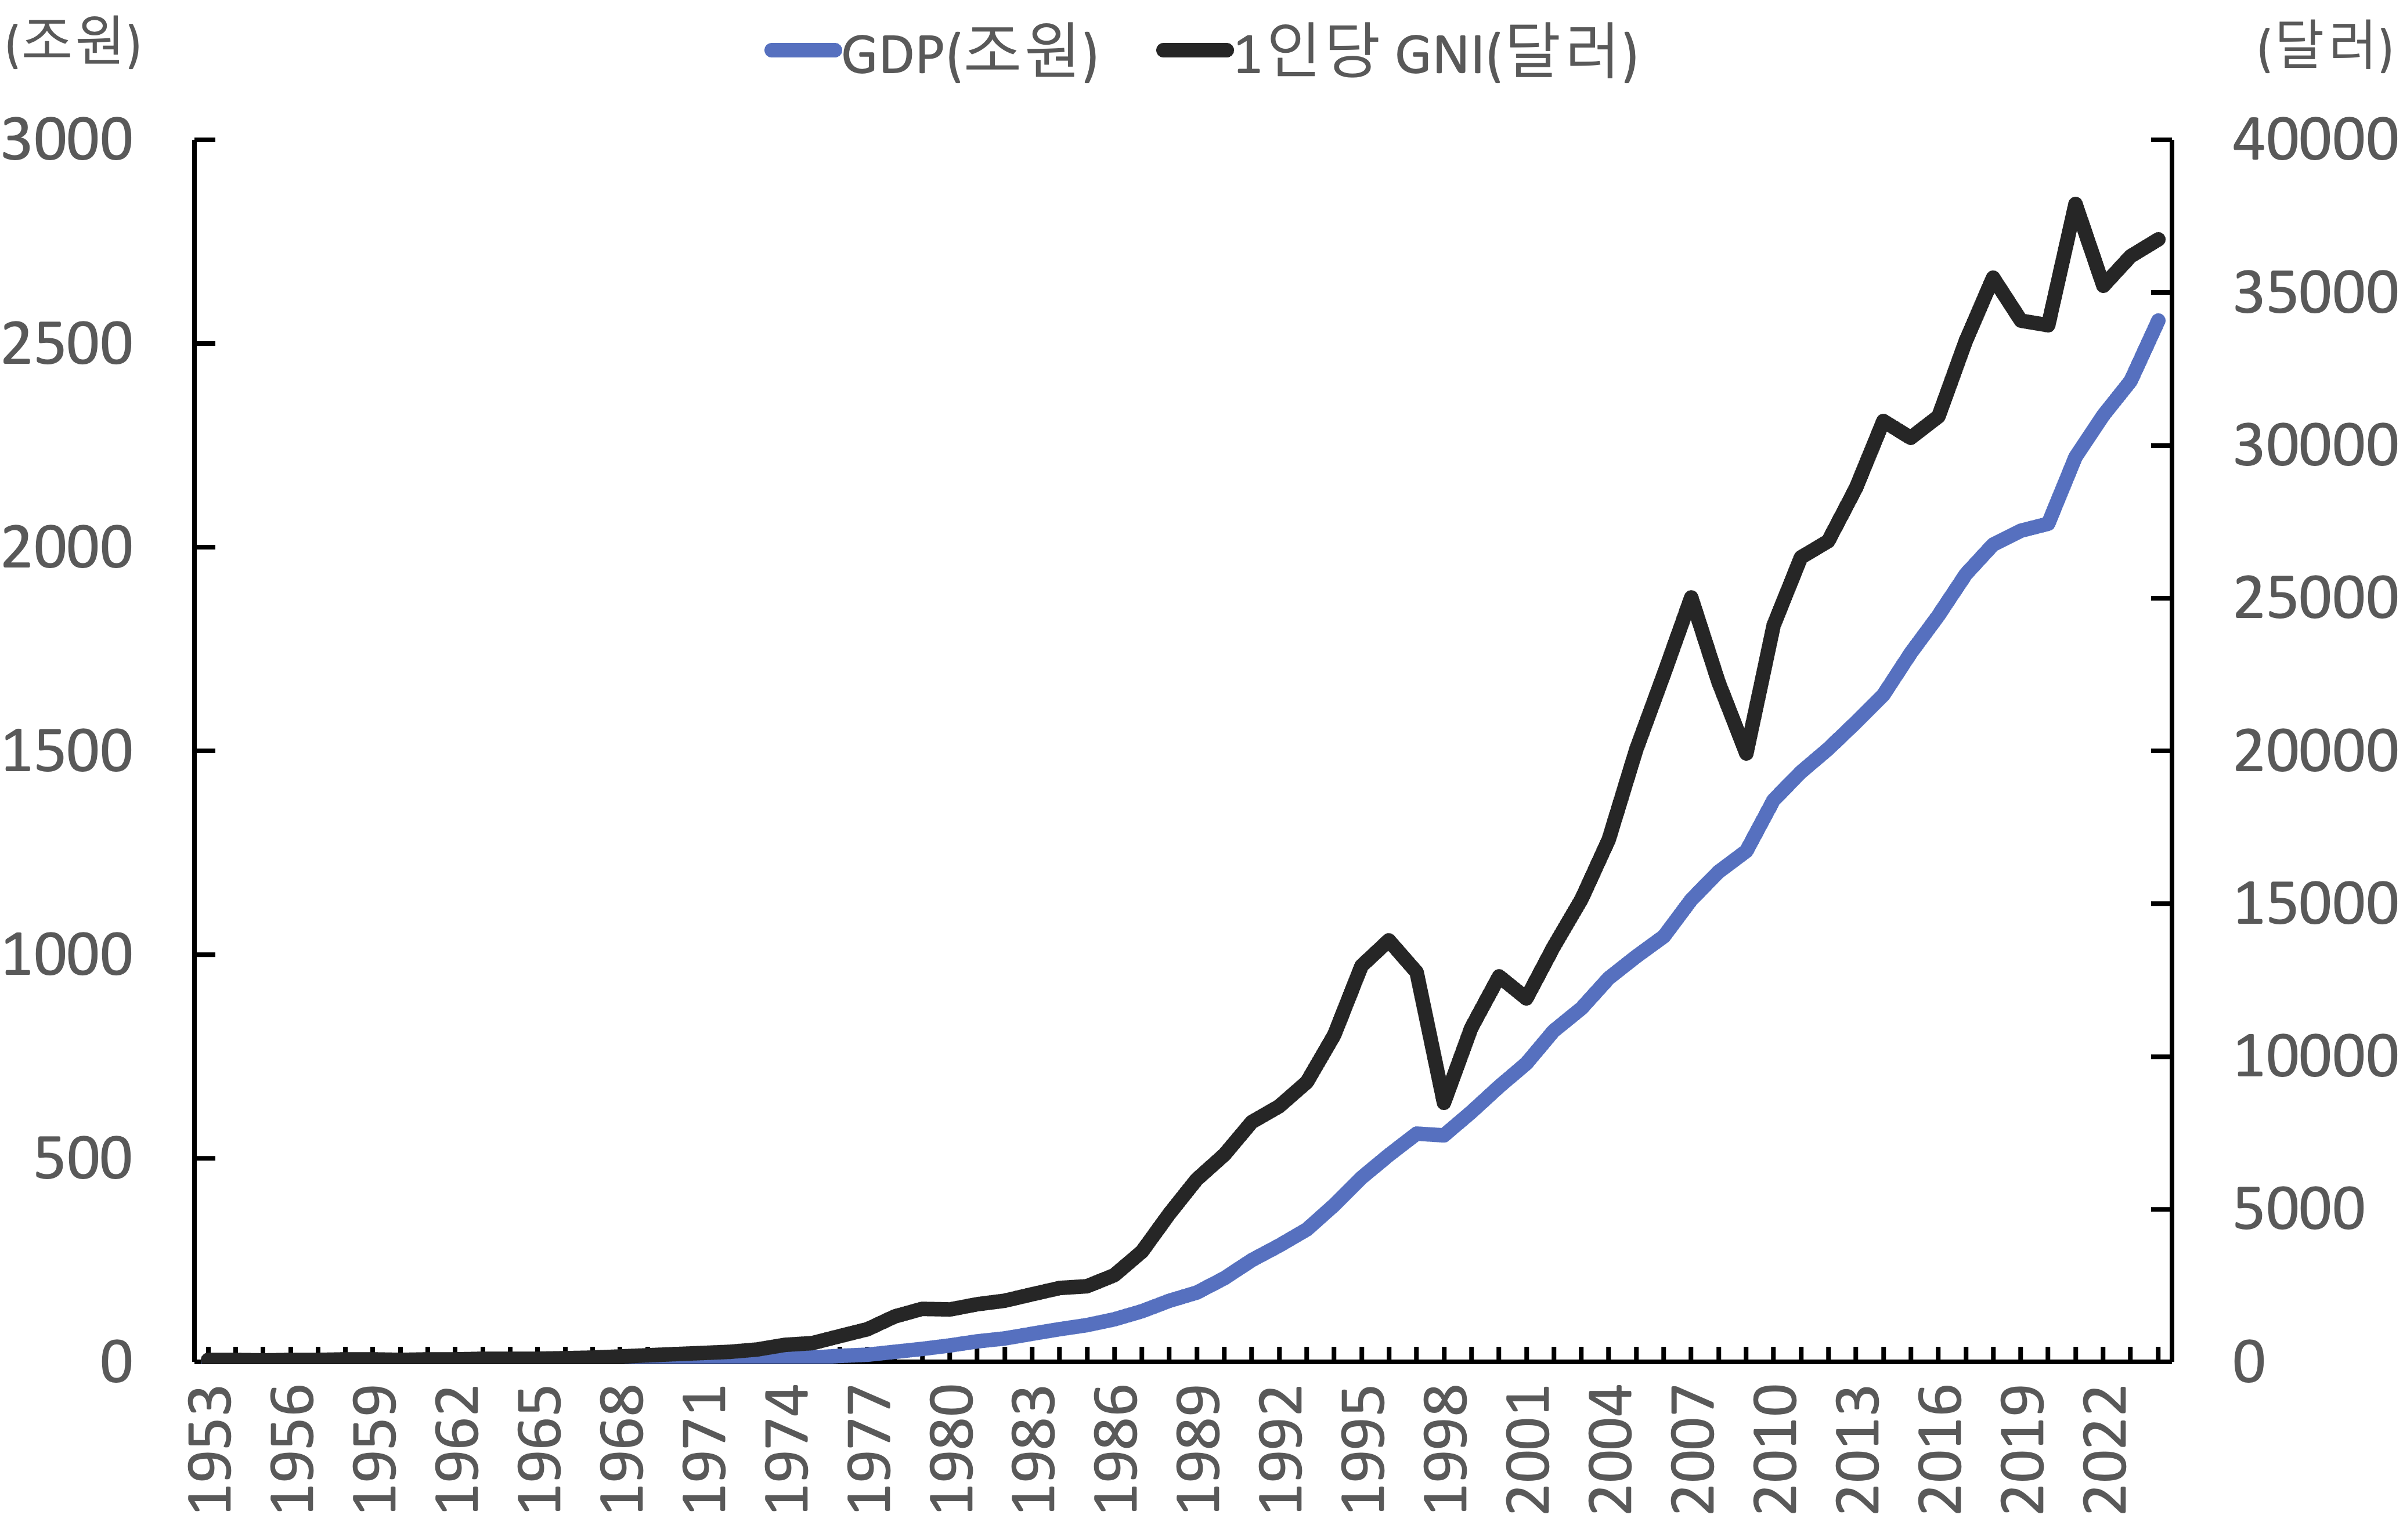
\includegraphics[width=.5\textwidth]{pic/fig_econ_01.png}
    \end{figure}
    \begin{itemize}
        \item 전쟁의 폐허 속에서 출발한 한국은 압축 성장을 통해 세계 10위권 경제와 1인당 소득 3만 6천 달러를 달성했다.
    \end{itemize}
\end{frame}

\begin{frame}[<+->]
\frametitle{고속성장의 기적을 지나 선진국형 저성장 시대로 접어들다.}
    \begin{figure}
        \centering
        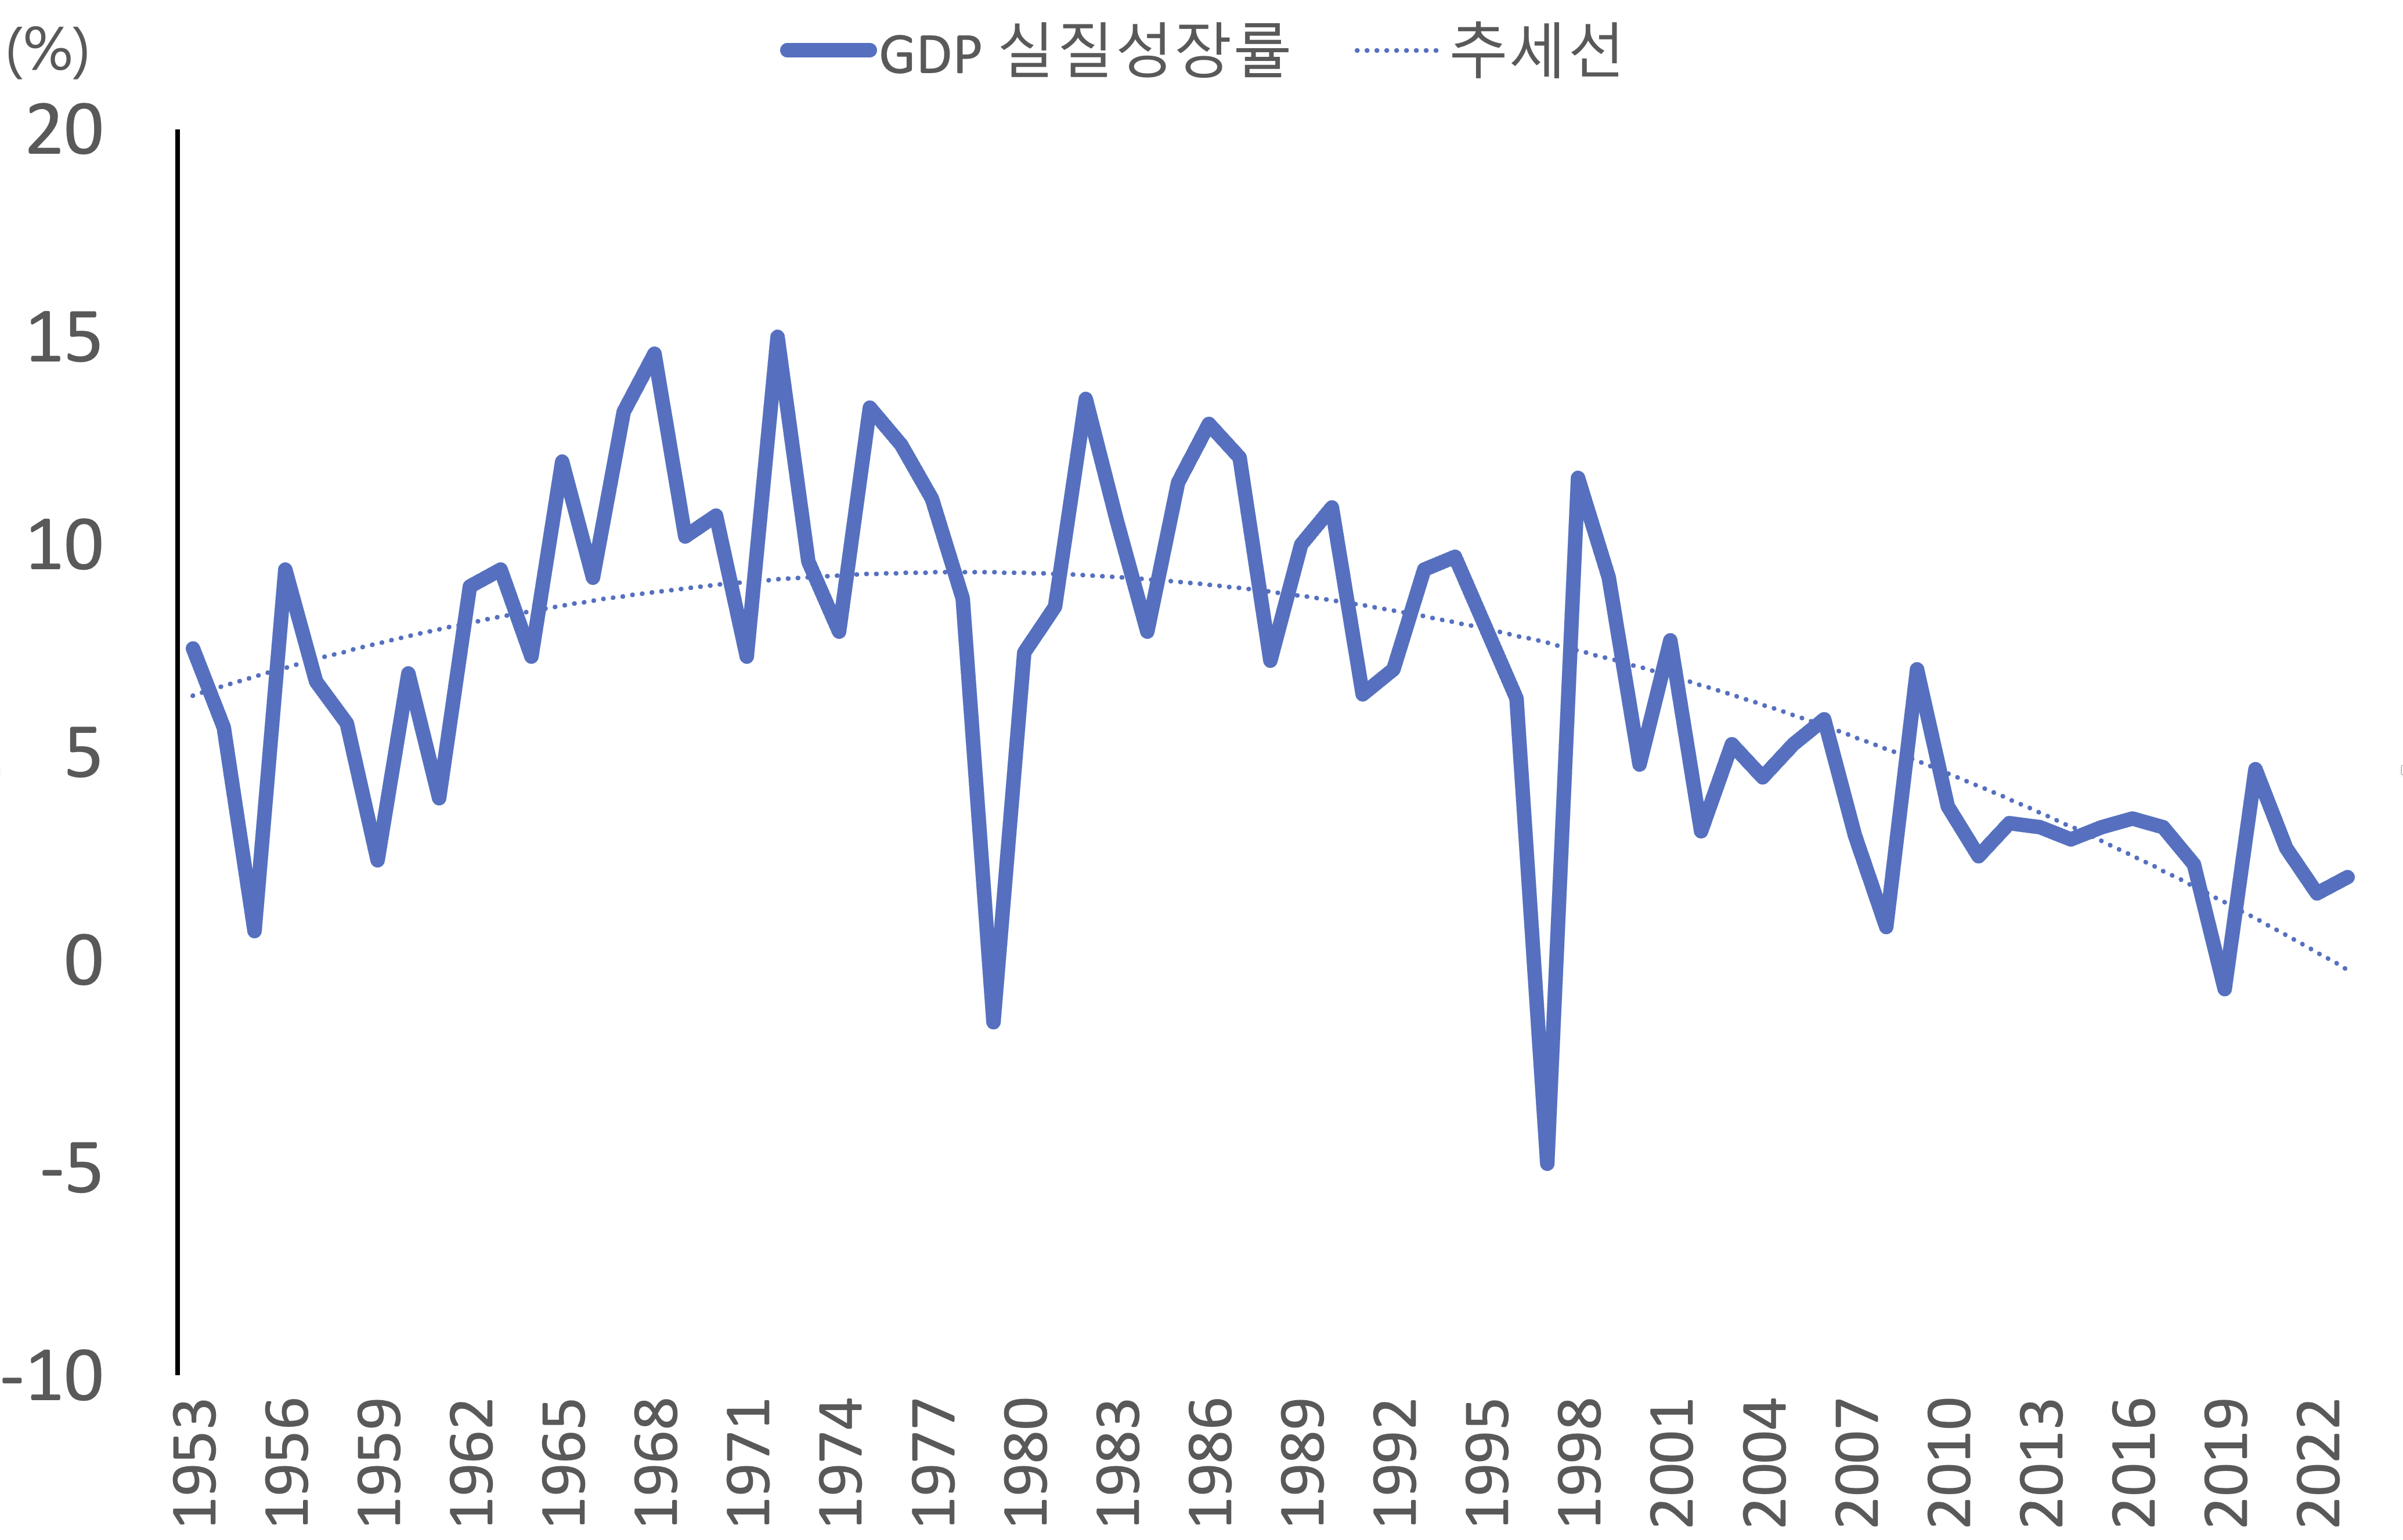
\includegraphics[width=.5\textwidth]{pic/fig_econ_02.png}
    \end{figure}
    \begin{itemize}
        \item 1960--80년대 두 자릿수 성장을 이어가던 한국경제는 수 차례의 위기를 훌륭히 극복해왔고, 이제는 안정된 저성장 시대에 접어들었다.
    \end{itemize}
\end{frame}

\subsection{산업구조}
\begin{frame}
\frametitle{농업 사회에서 제조업과 서비스 강국으로 탈바꿈 하다.}
\begin{columns}
    \begin{column}{.5\textwidth}
        \begin{figure}
            \centering
            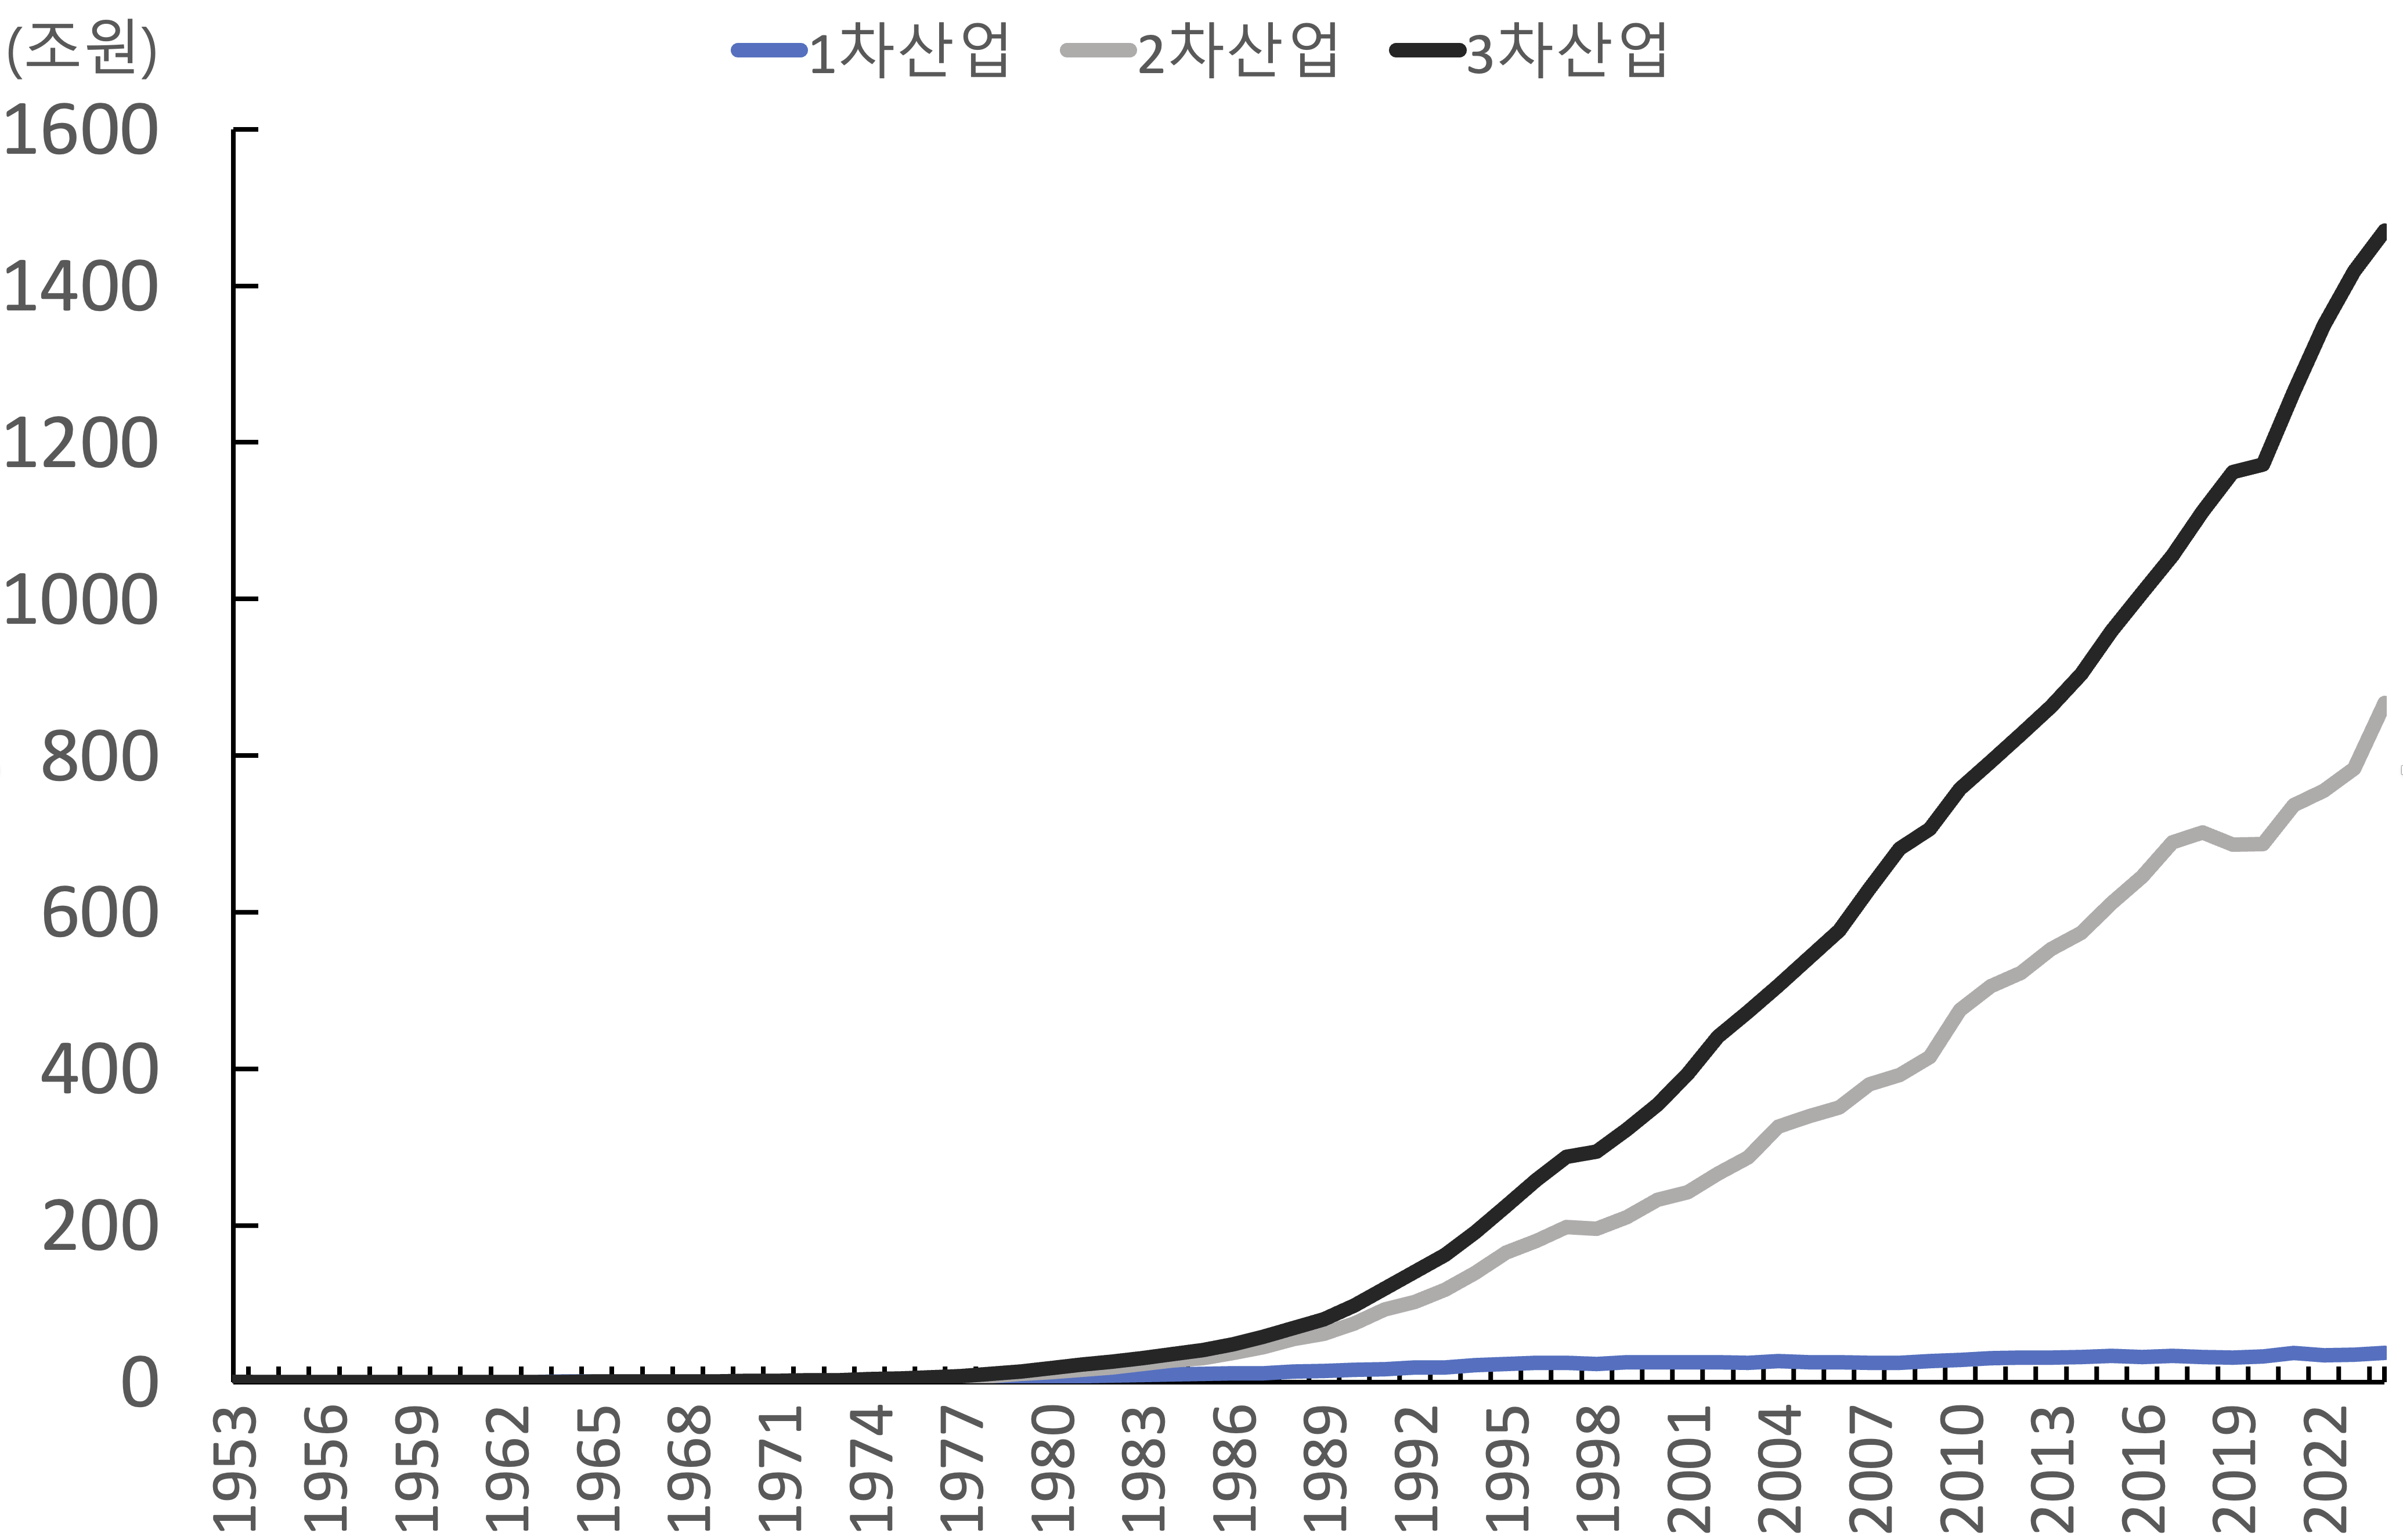
\includegraphics[width=.8\textwidth]{pic/fig_econ_03.png}
        \end{figure}
        \begin{itemize}[<+->]
            \item 70년대 부터 2차산업이 빠르게 성장했고, 80년대 이후부터는 3차산업 역시 성장하기 시작한다.
        \end{itemize}
    \end{column}
    \begin{column}{.5\textwidth}
        \begin{figure}
            \centering
            \only<1|handout:0>{\transparent{0.3}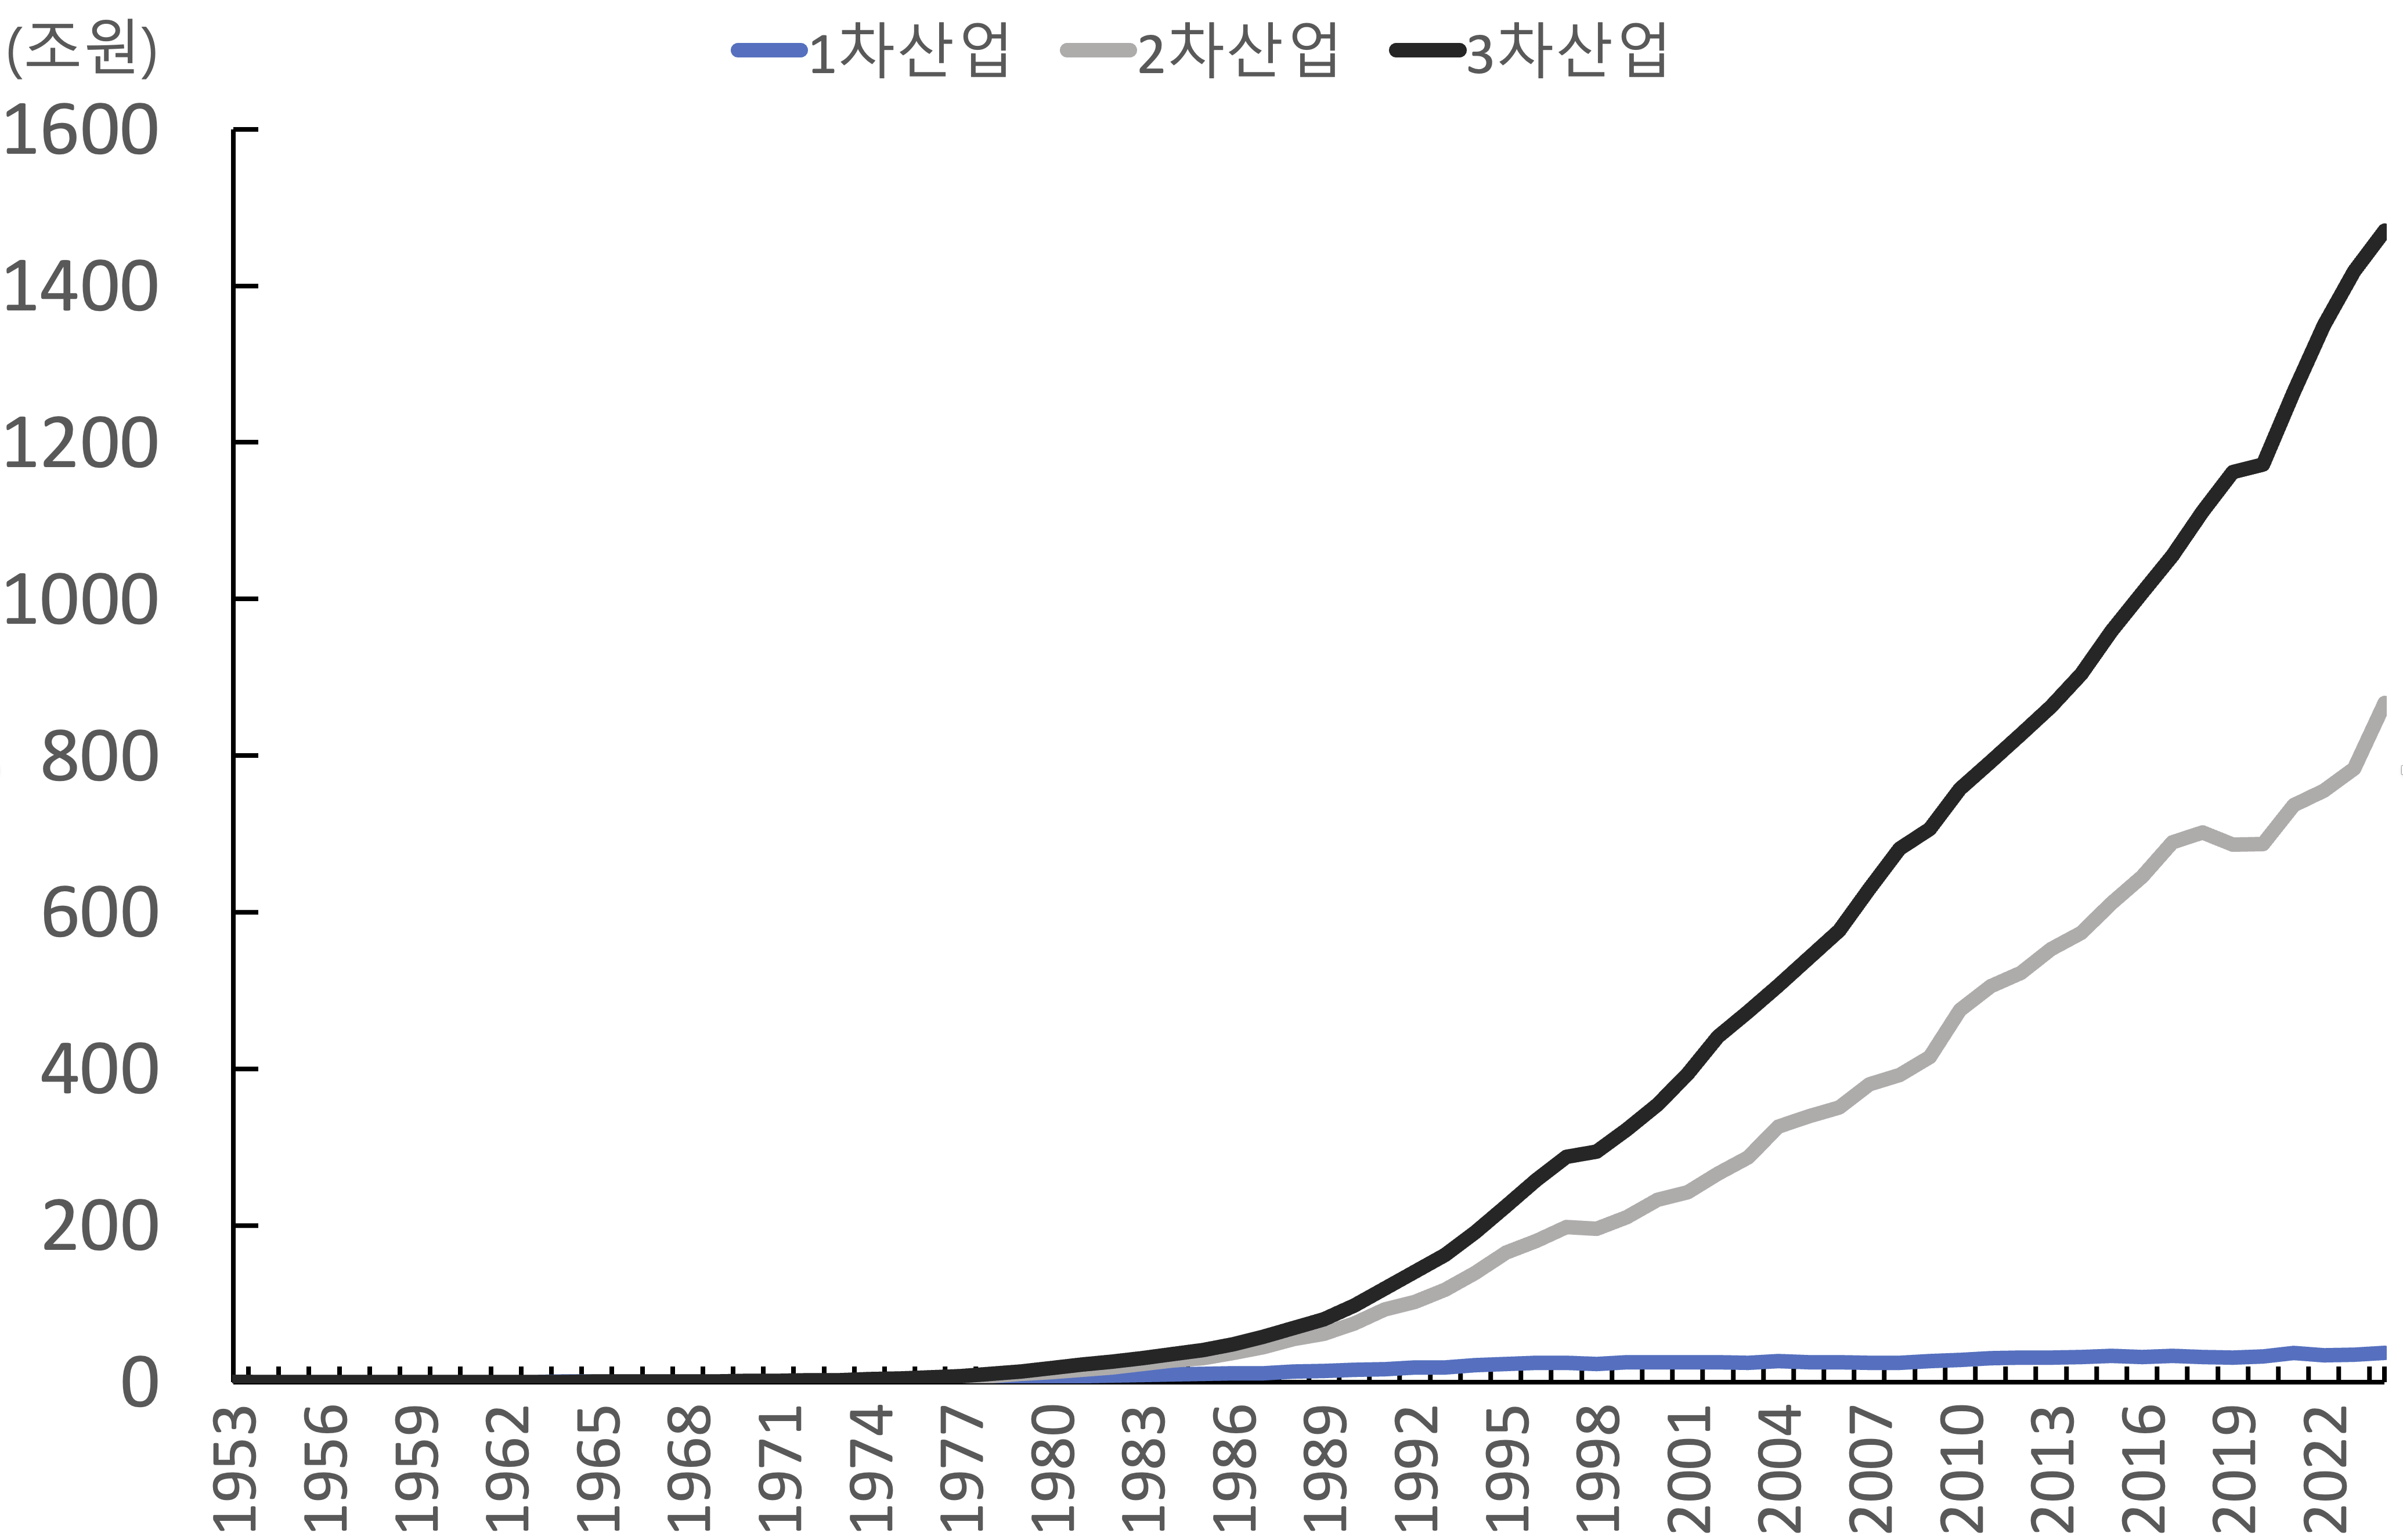
\includegraphics[width=.8\textwidth]{pic/fig_econ_03.png}} % 첫 번째 슬라이드: 투명하게 표시
            \only<2>{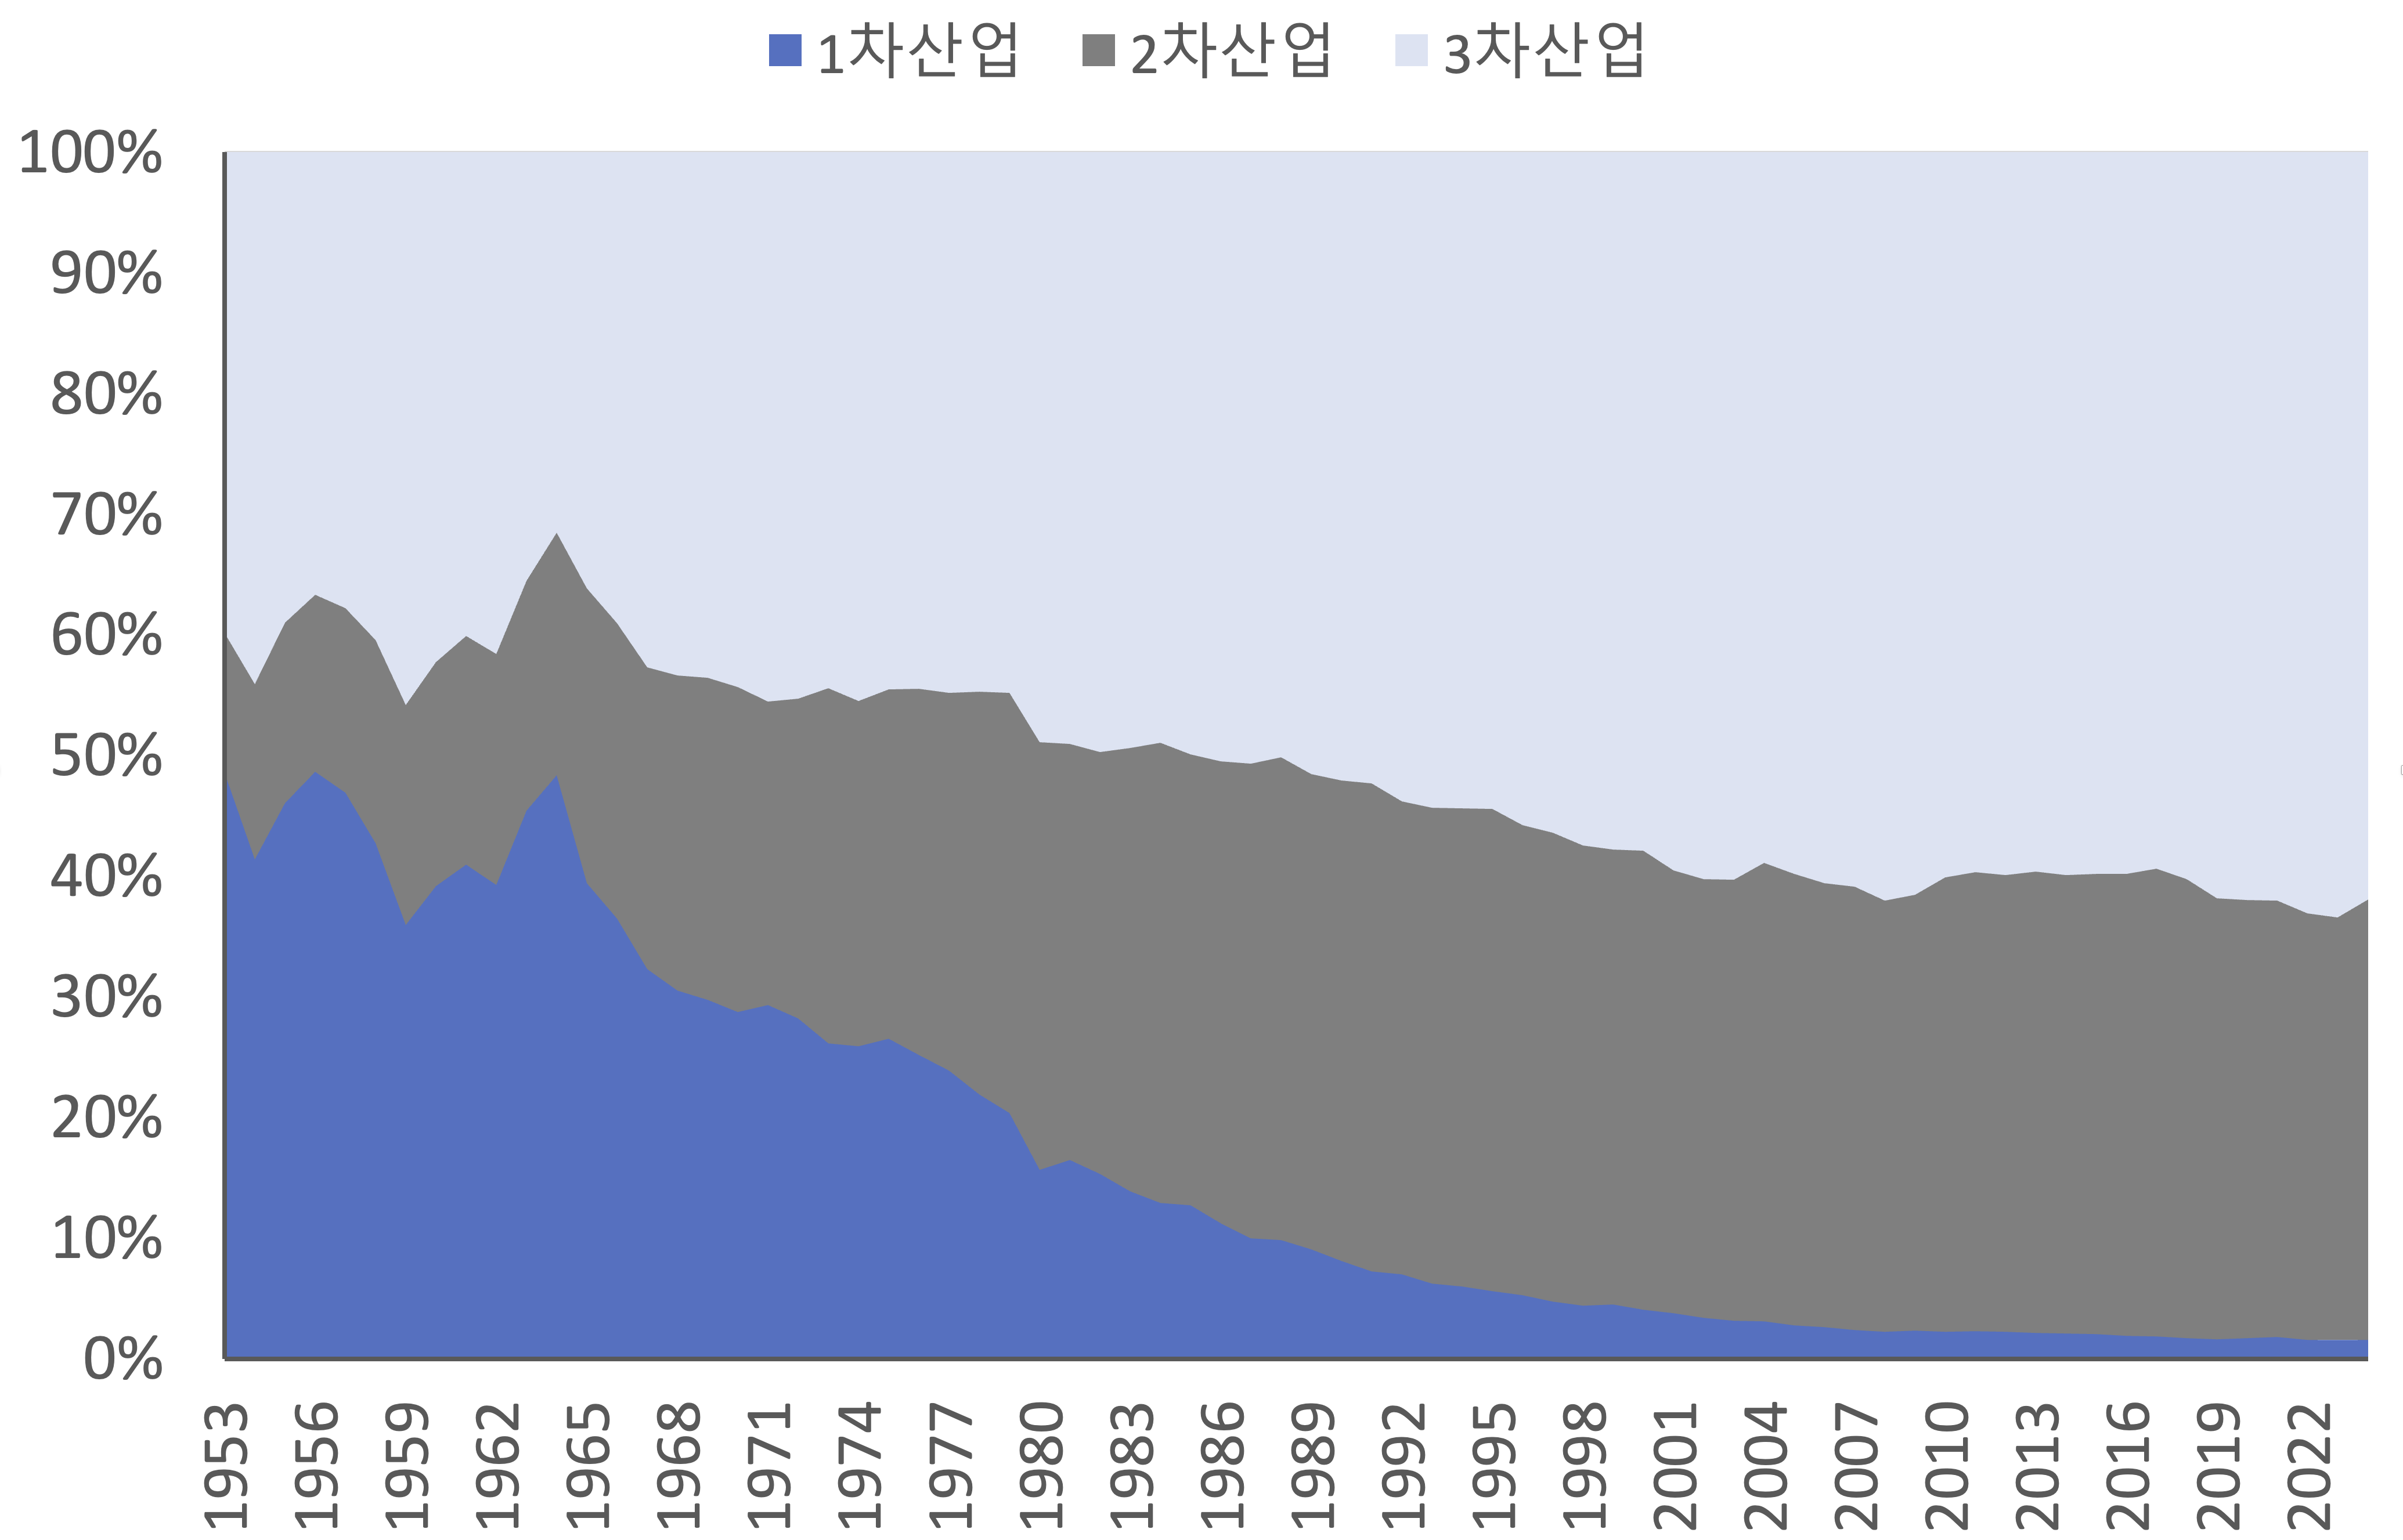
\includegraphics[width=.8\textwidth]{pic/fig_econ_04.png}} % 두 번째 슬라이드: 선명하게 표시
            \\
            \begin{itemize}[<+->]
                \item 농업이 주축이던 경제는 제조업의 고도화를 거쳐 서비스업이 중심이 되는 선진국형 구조로 바뀌었다.
            \end{itemize}
        \end{figure}
    \end{column}
\end{columns}
\end{frame}

\subsection{무역}
\begin{frame}[<+->]
\frametitle{원자재에서 섬유류를 거쳐 반도체·자동차까지, 수출 강국으로 성장하다.}
    \begin{figure}
        \centering
        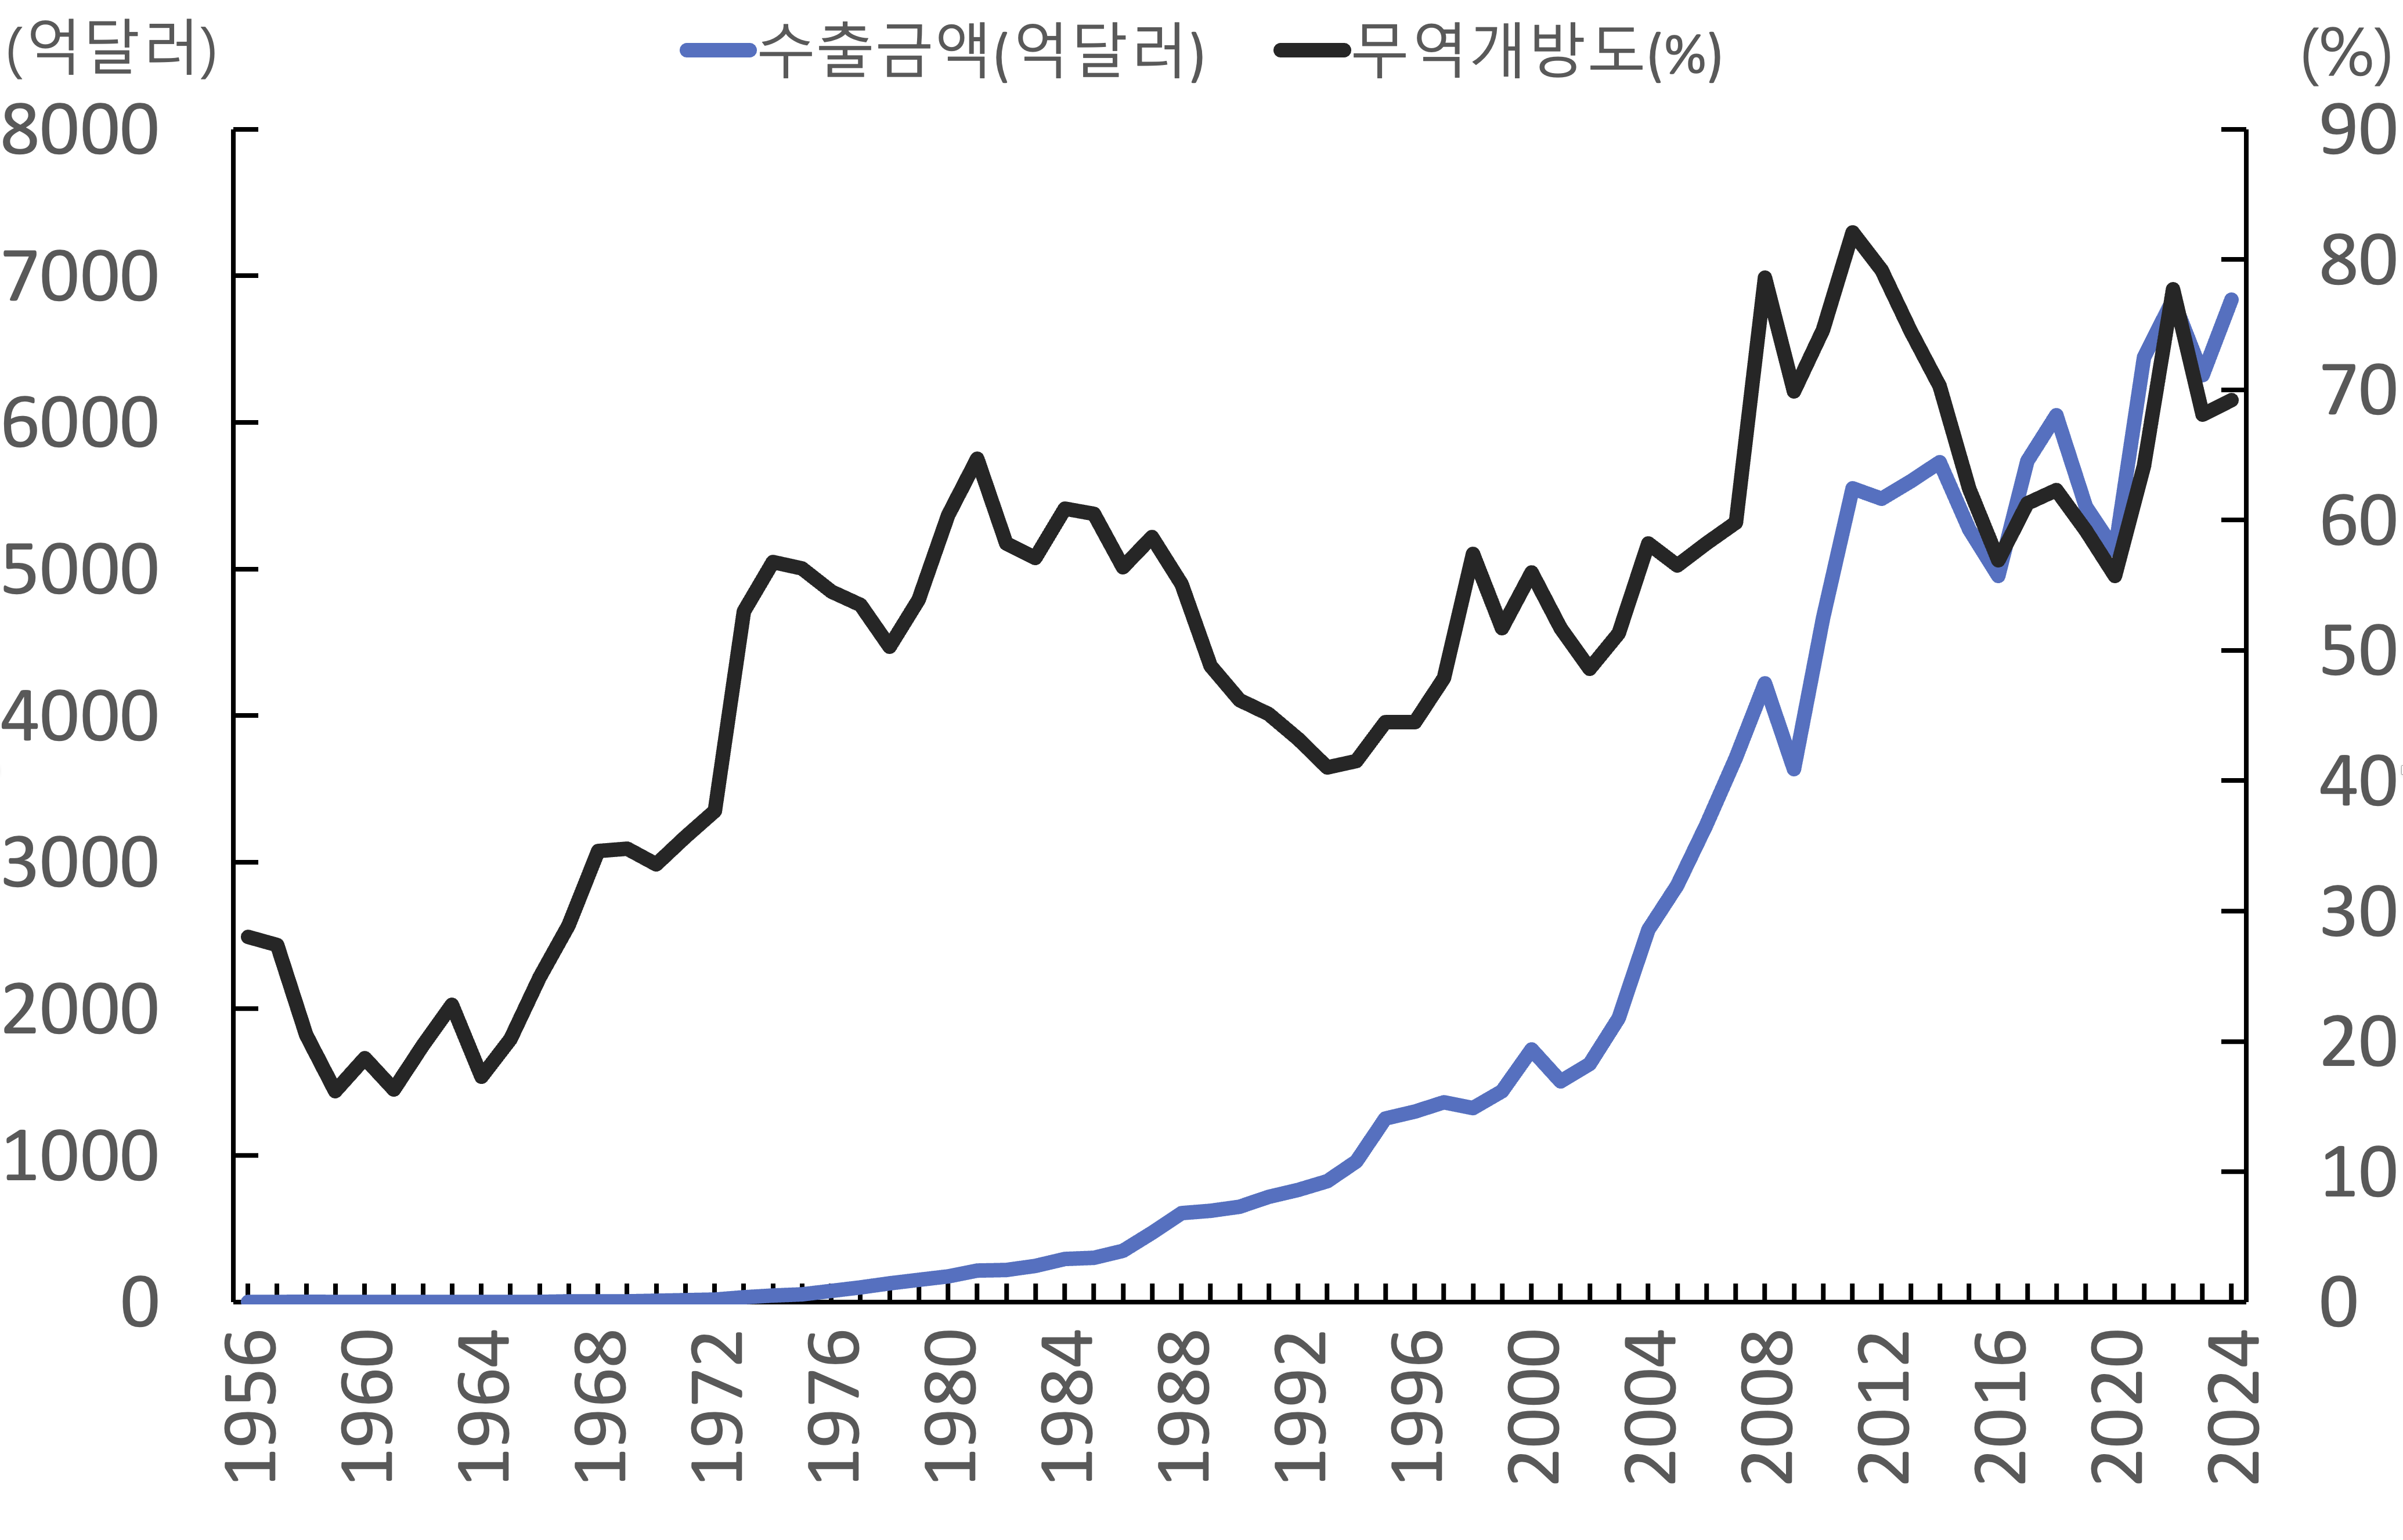
\includegraphics[width=.5\textwidth]{pic/fig_econ_05.png}
    \end{figure}
    \begin{itemize}
        \item 한국은 산업고도화 동시에 수출주도 성장전략을 채택했다. 원자재 위주의 수출은 첨단산업 제품 중심으로 재편되며 한국을 세계 6위권 수출대국으로 이끌었다.
    \end{itemize}
\end{frame}

\begin{frame}
\frametitle{무역 적자와 원조 의존국에서 흑자와 공여국으로 전환하다.}
\begin{columns}
    \begin{column}{.5\textwidth}
        \begin{figure}
            \centering
            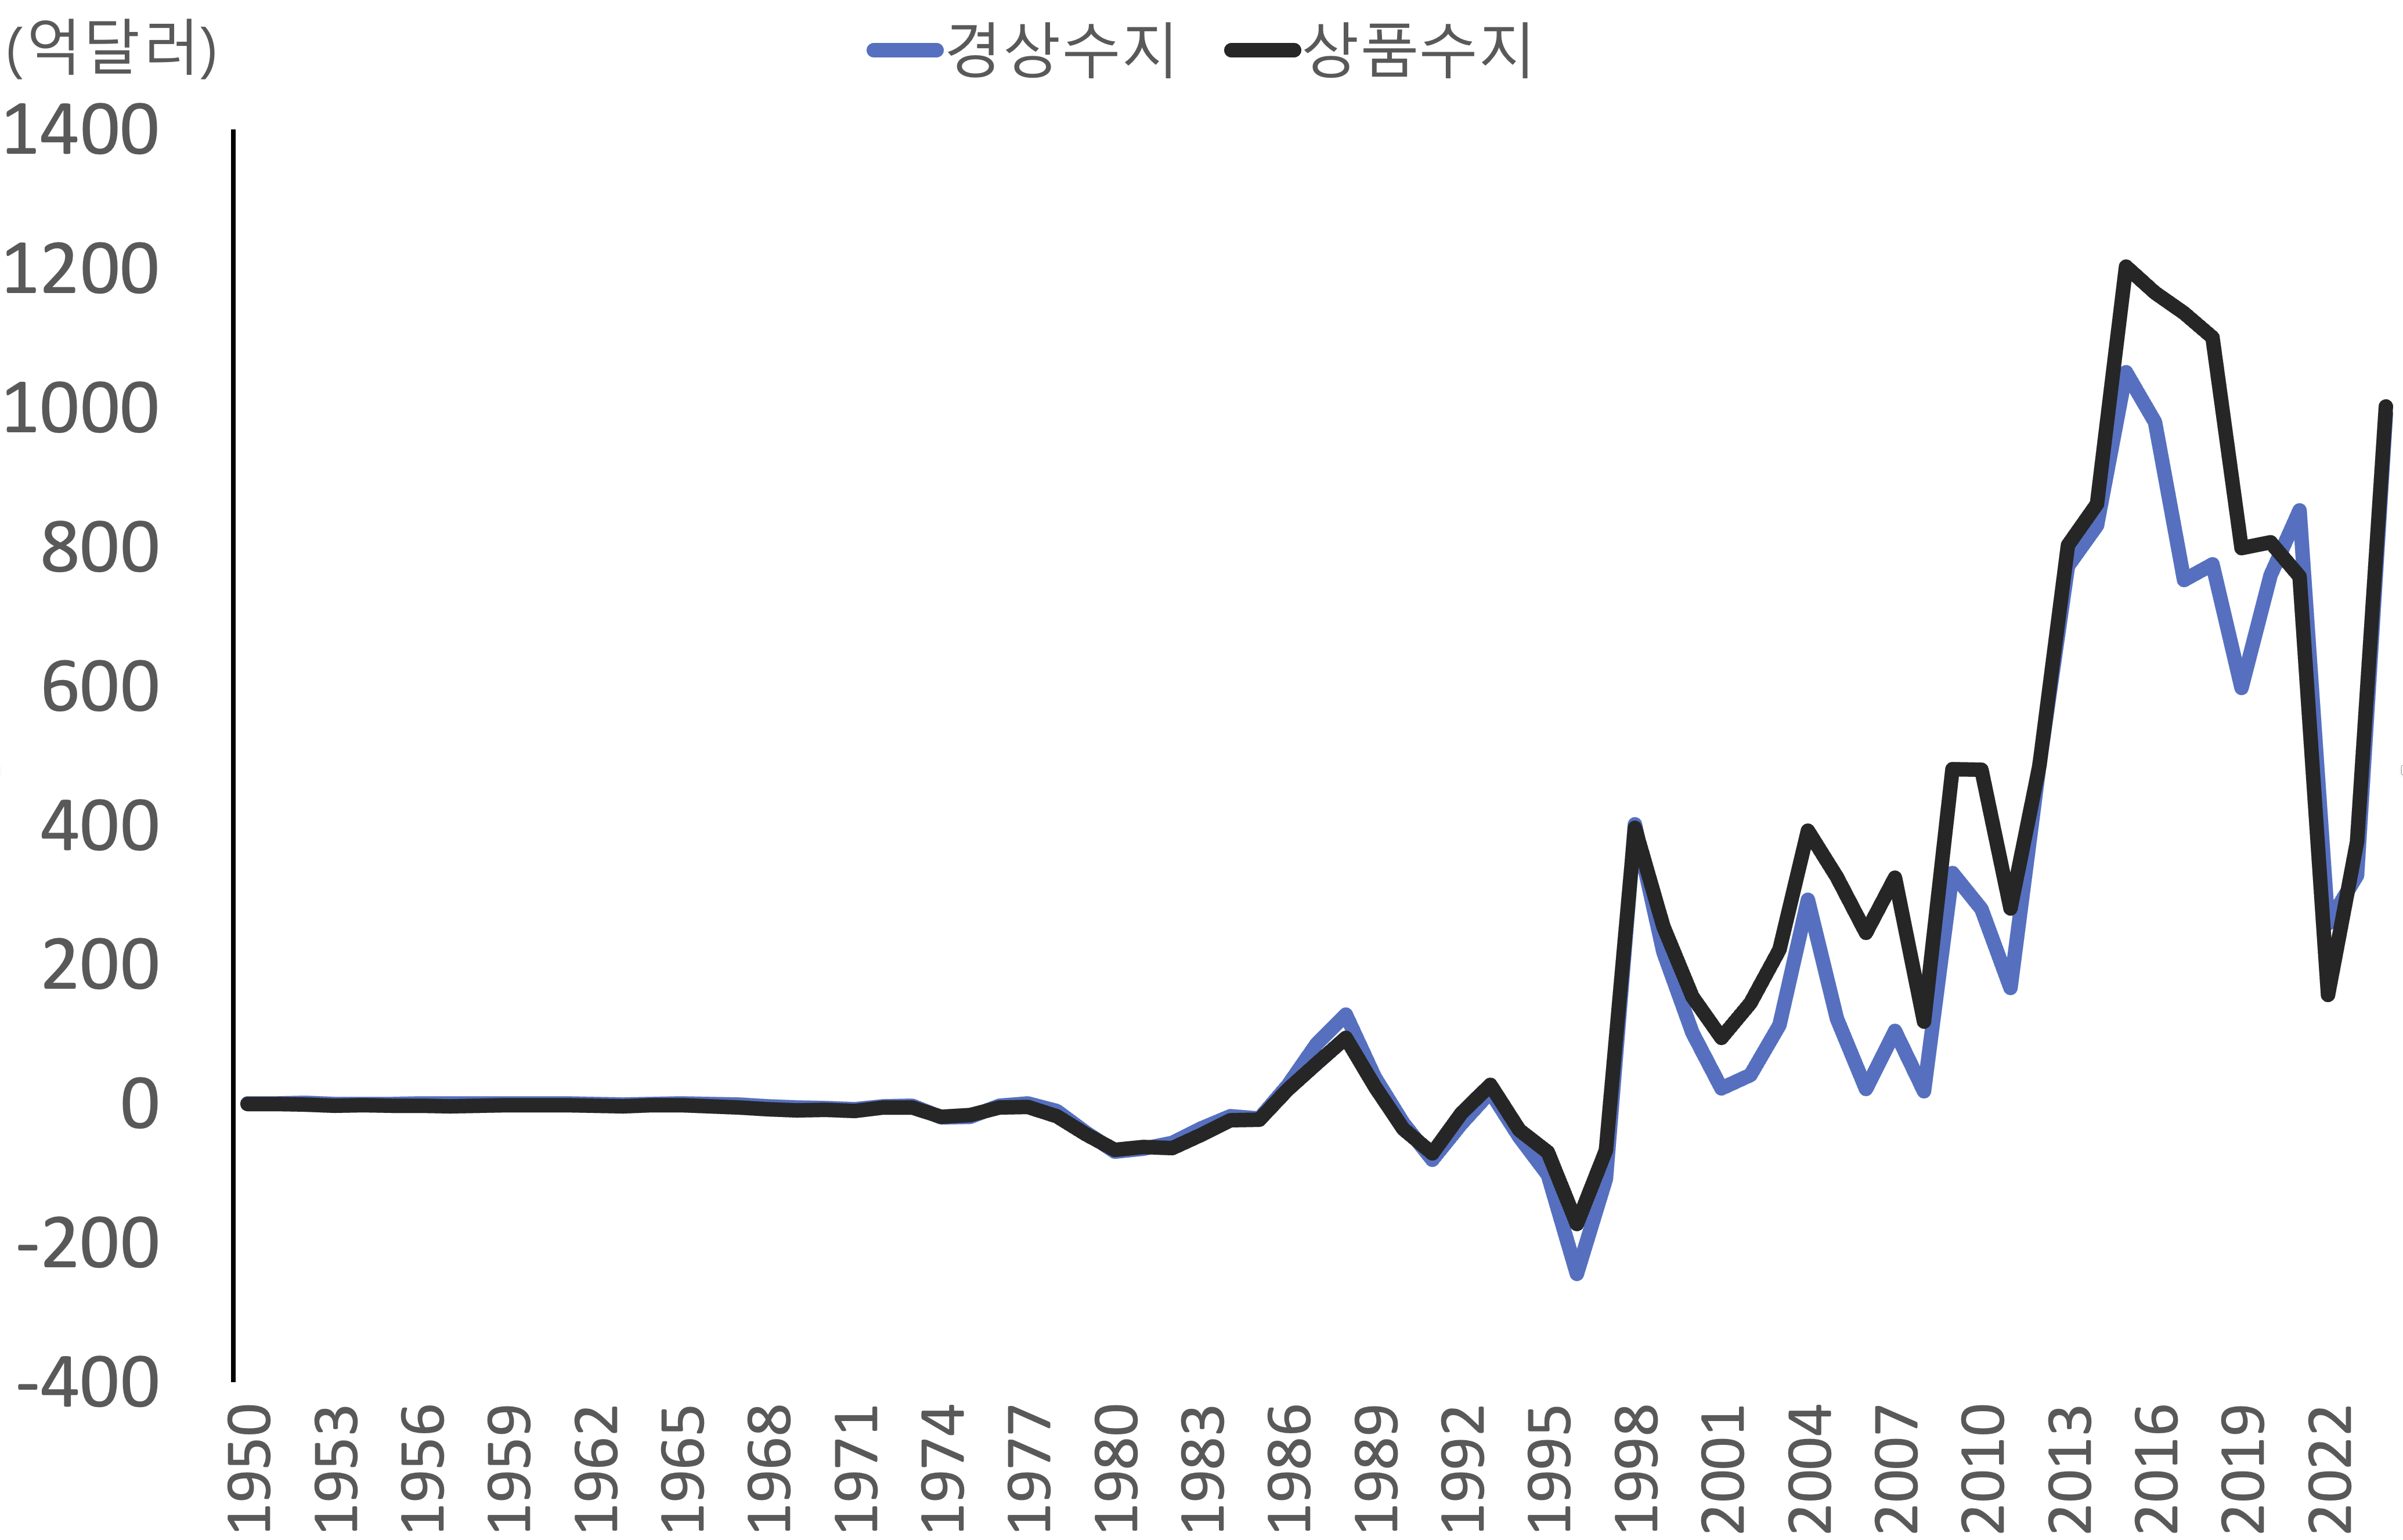
\includegraphics[width=.8\textwidth]{pic/fig_econ_06.png}
        \end{figure}
        \begin{itemize}[<+->]
            \item 1986년 처음으로 경상수지 흑자를 달성했고, 현재는 경상수지 흑자 국가가 되었다.
        \end{itemize}
    \end{column}
    \begin{column}{.5\textwidth}
        \begin{figure}
            \centering
            \only<1|handout:0>{\transparent{0.3}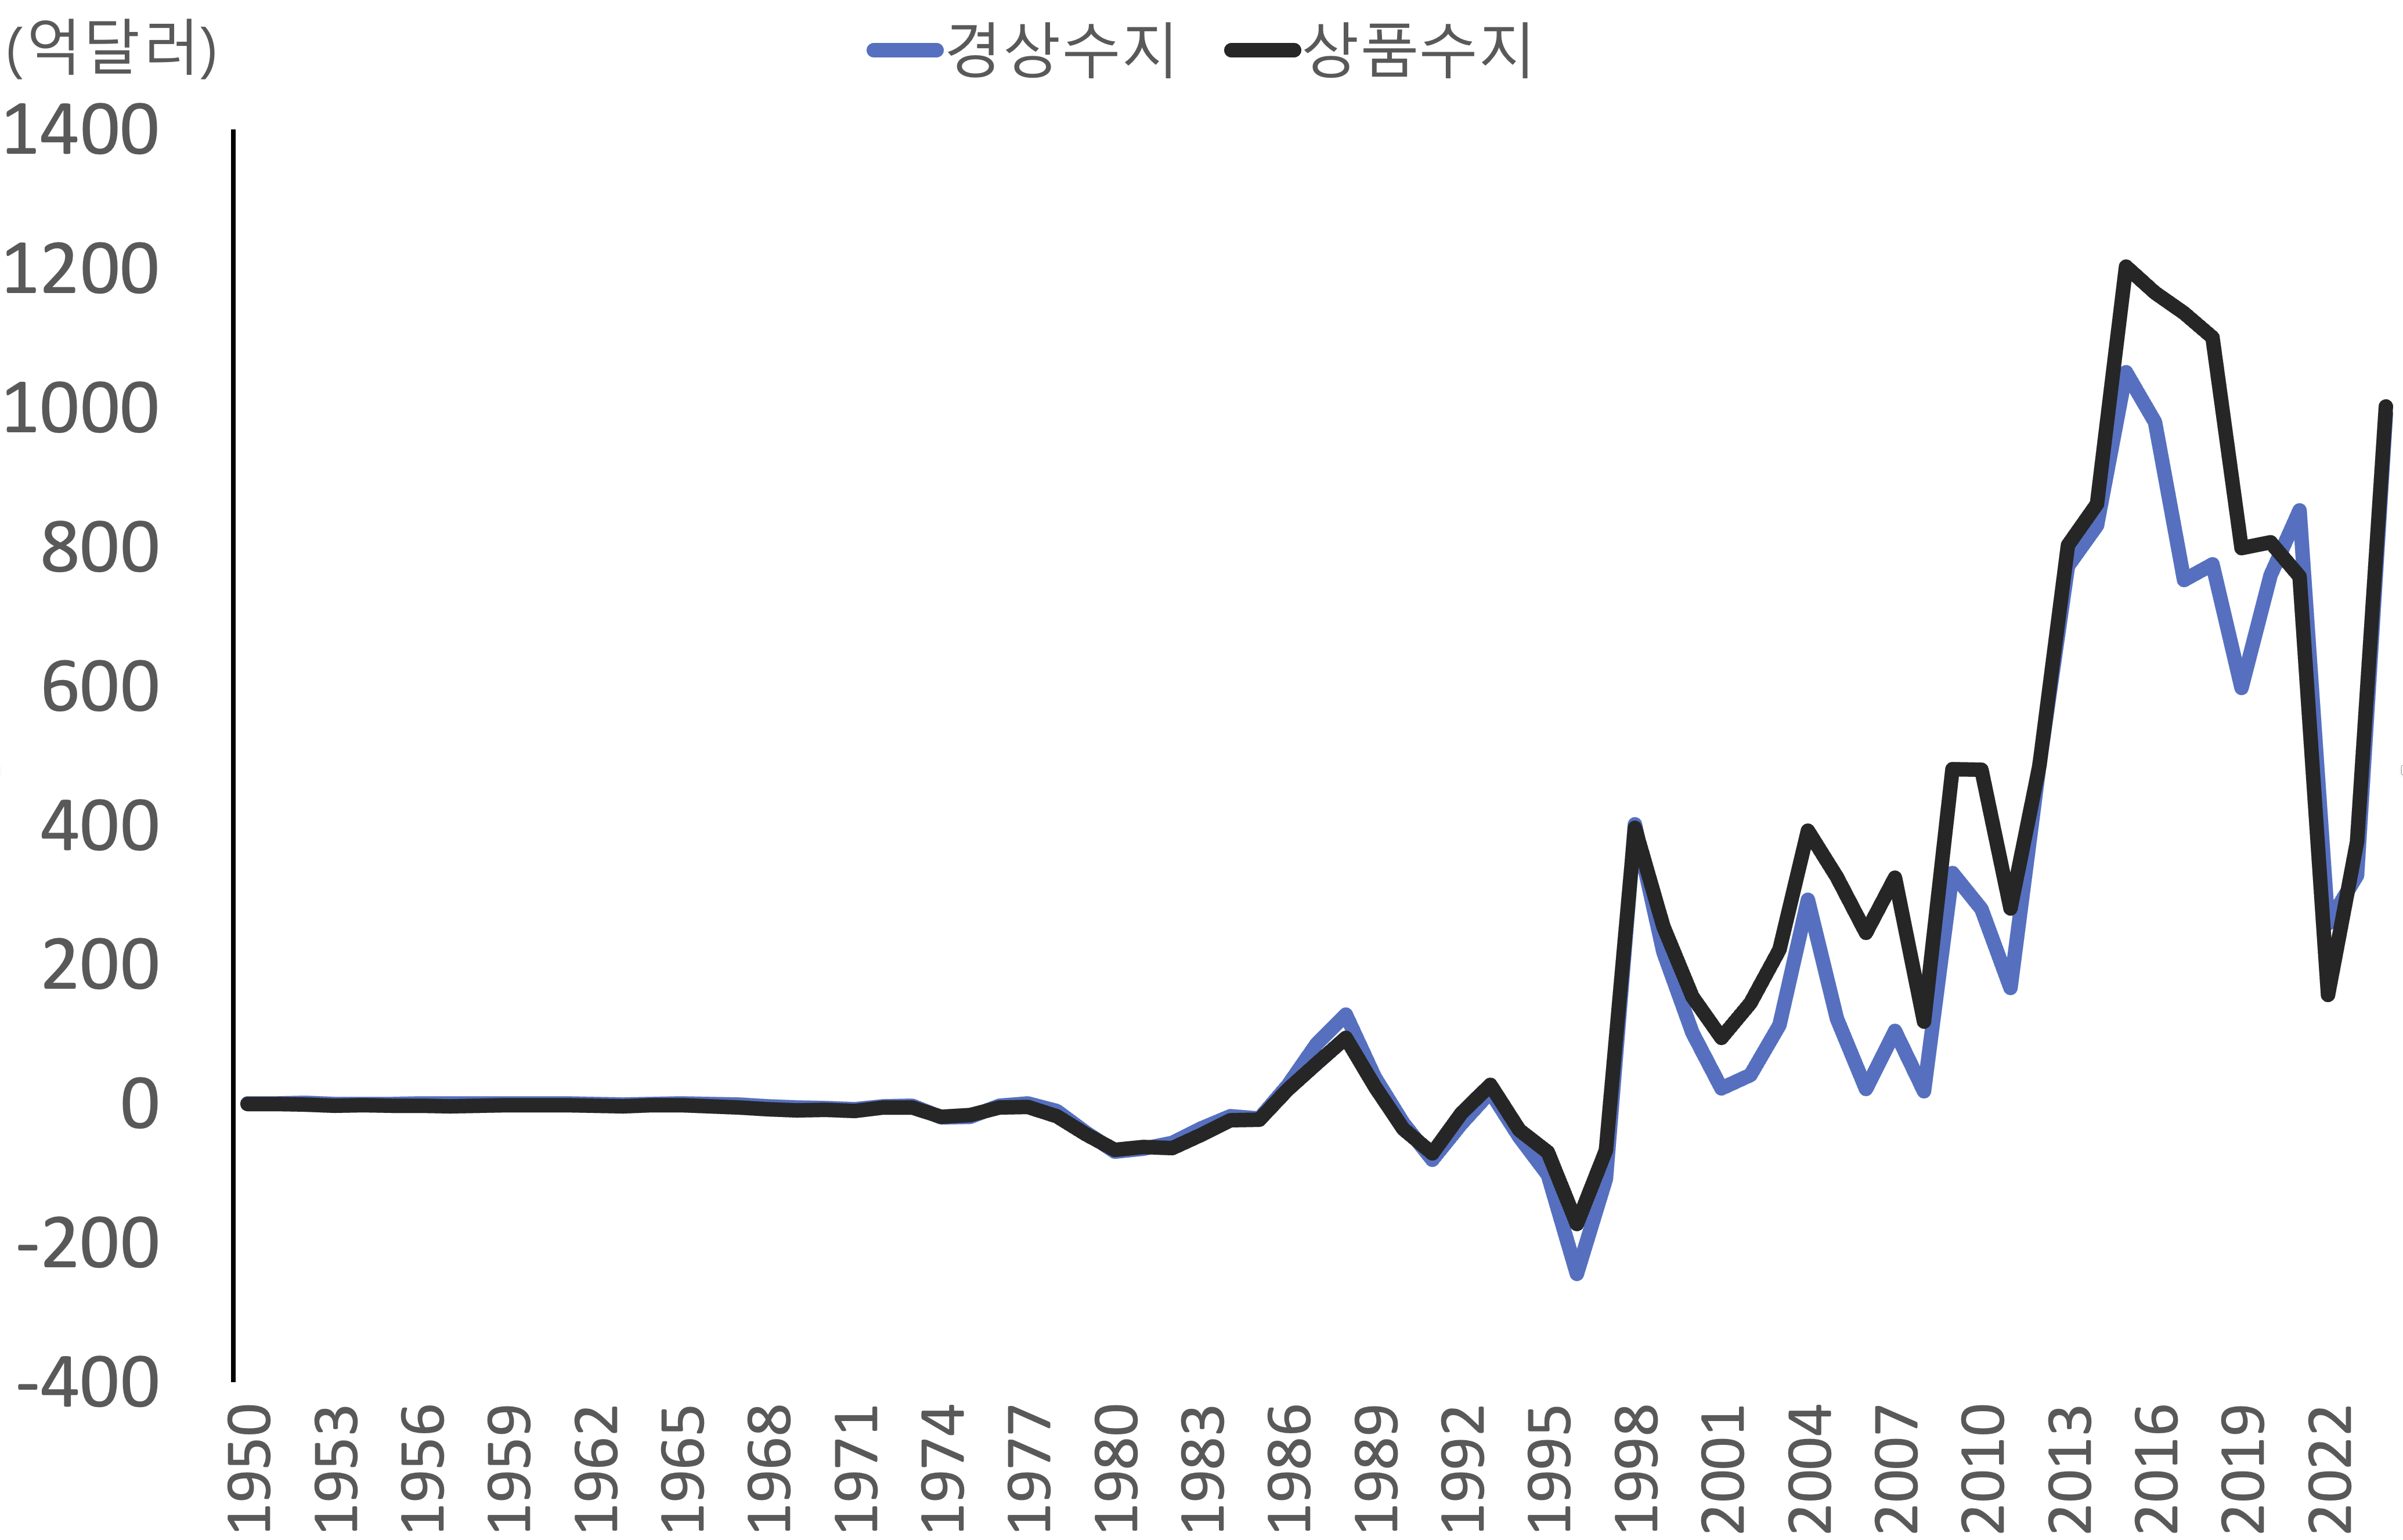
\includegraphics[width=.8\textwidth]{pic/fig_econ_06.png}} % 첫 번째 슬라이드: 투명하게 표시
            \only<2>{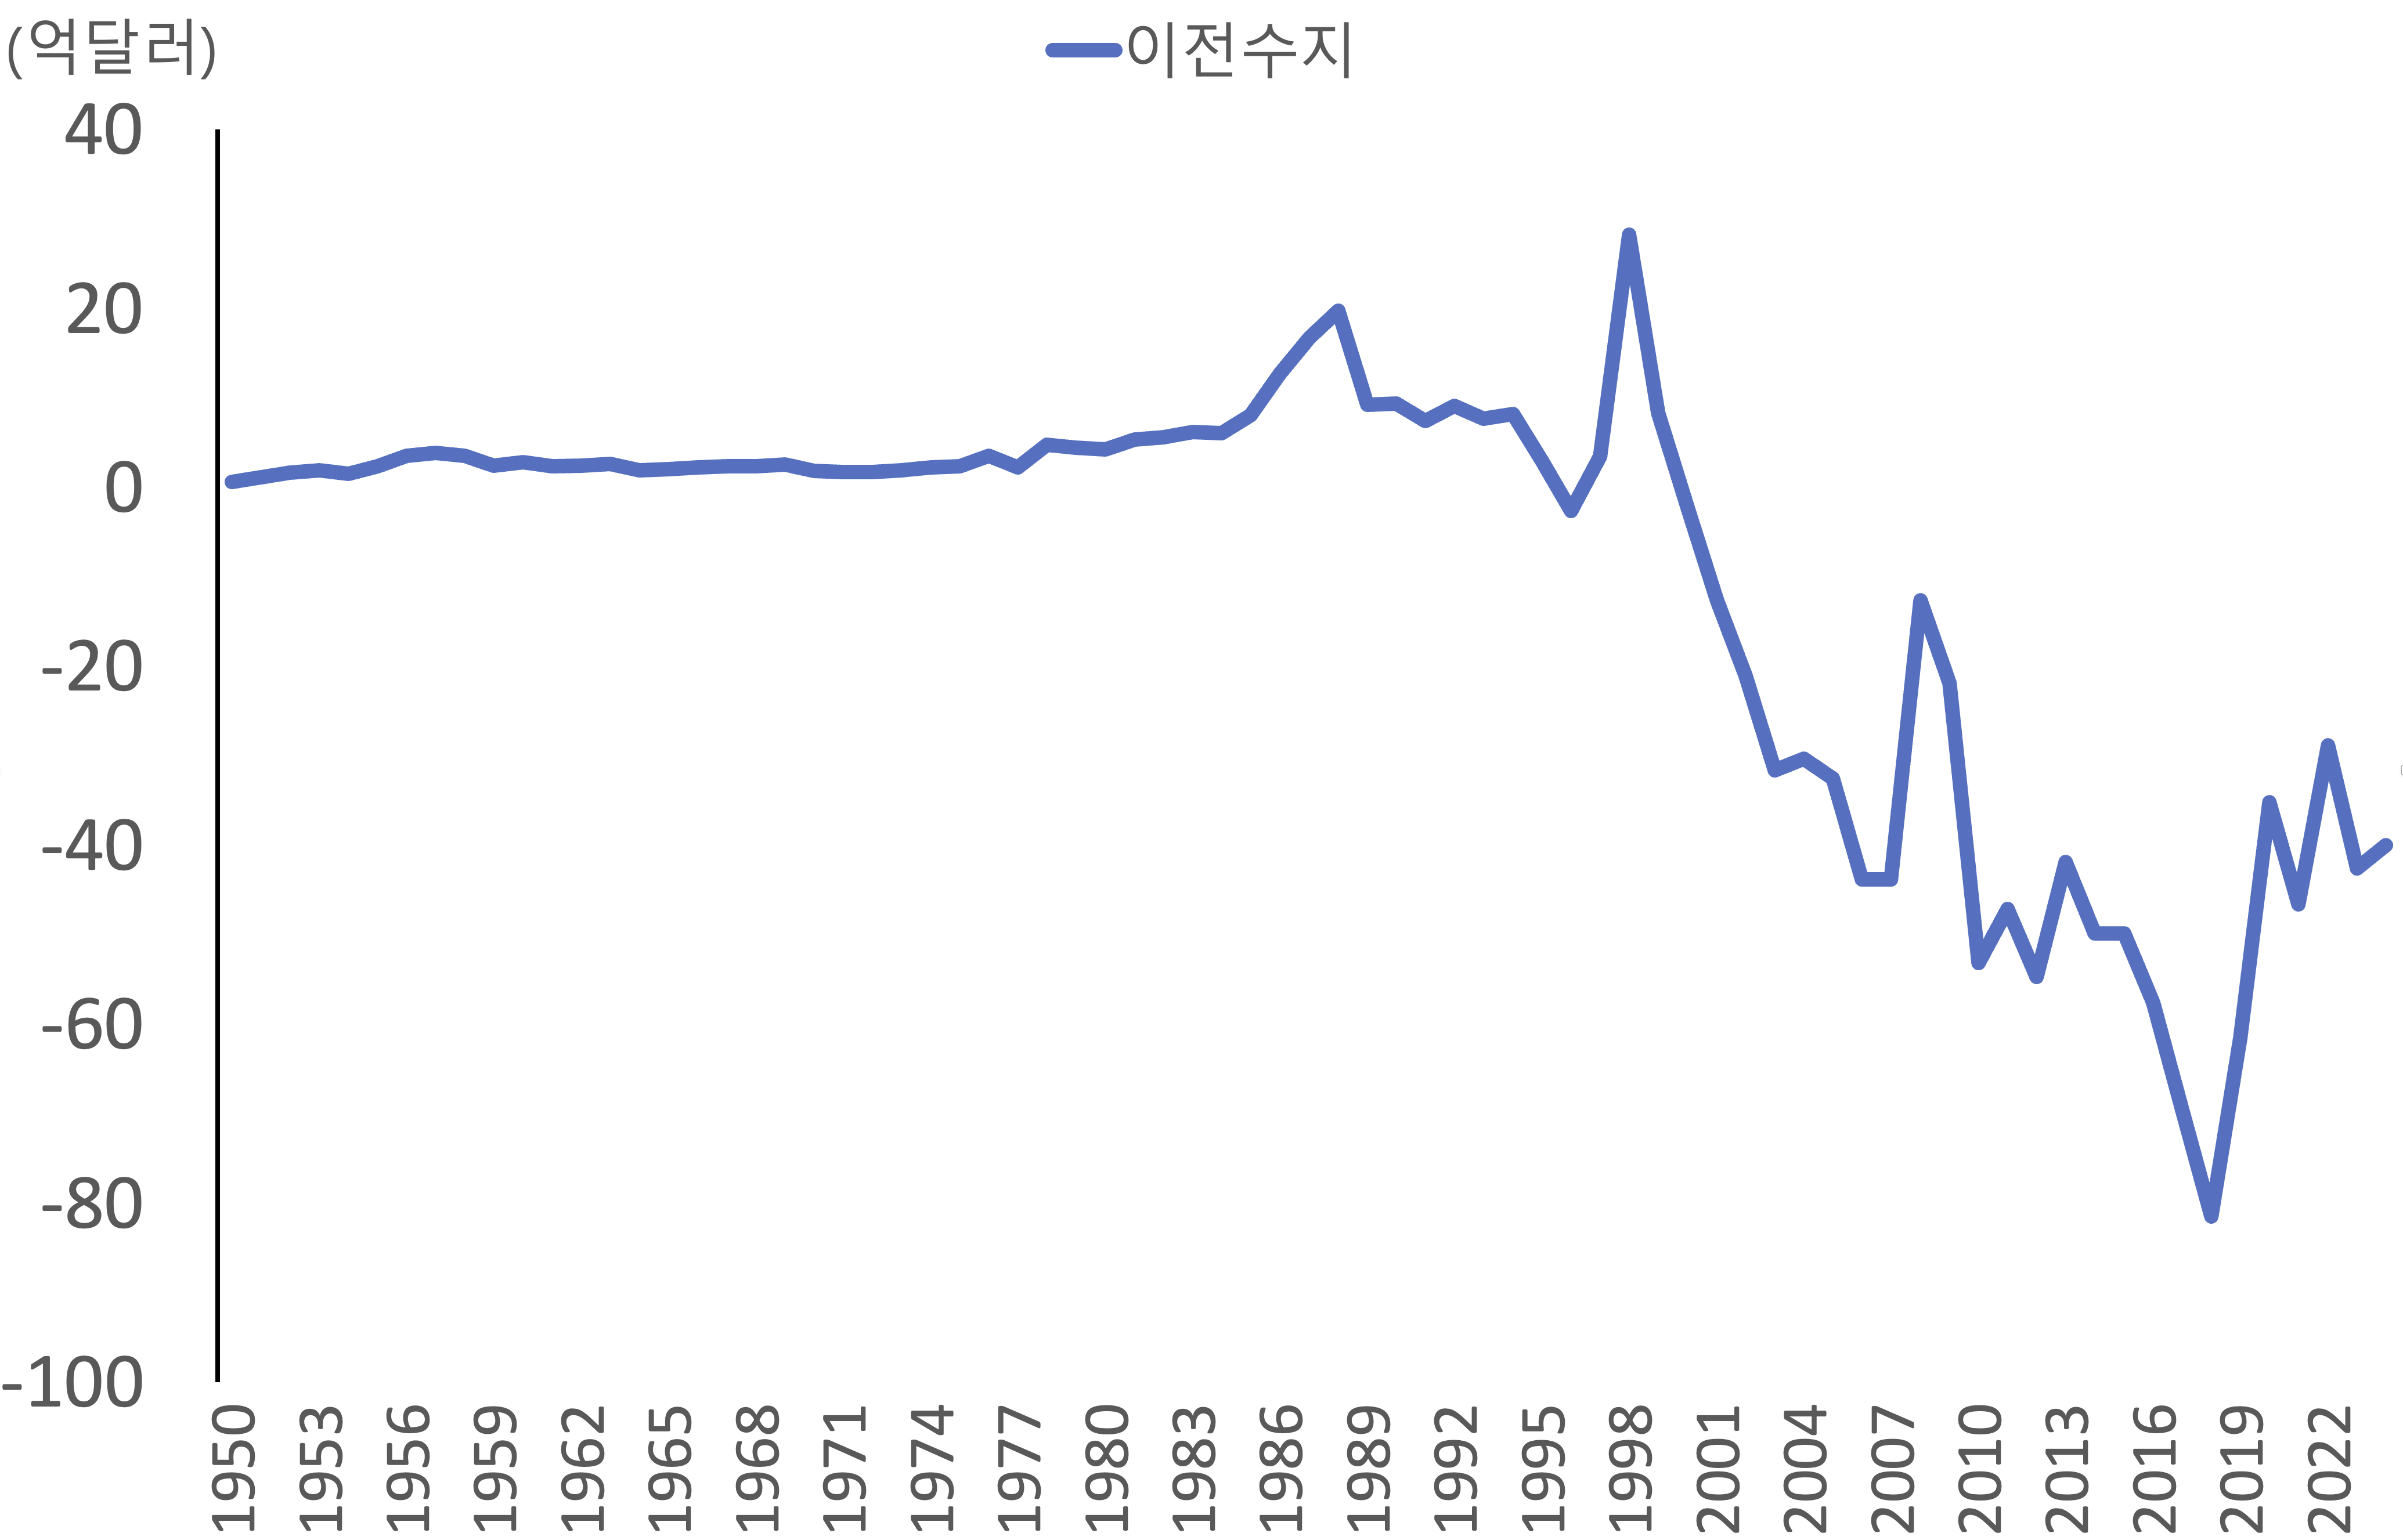
\includegraphics[width=.8\textwidth]{pic/fig_econ_07.png}} % 두 번째 슬라이드: 선명하게 표시
            \\
            \begin{itemize}[<+->]
                \item 2000년 이후 이전수지 적자를 기록하며 국제 원조를 제공하는 나라로 자리매김했다.
            \end{itemize}
        \end{figure}
    \end{column}
\end{columns}
\end{frame}

\subsection{외환}
\begin{frame}
\frametitle{외환위기의 교훈으로 외환보유액을 쌓고 환율 자유화를 이뤄냈다.}
\begin{columns}
    \begin{column}{.5\textwidth}
        \begin{figure}
            \centering
            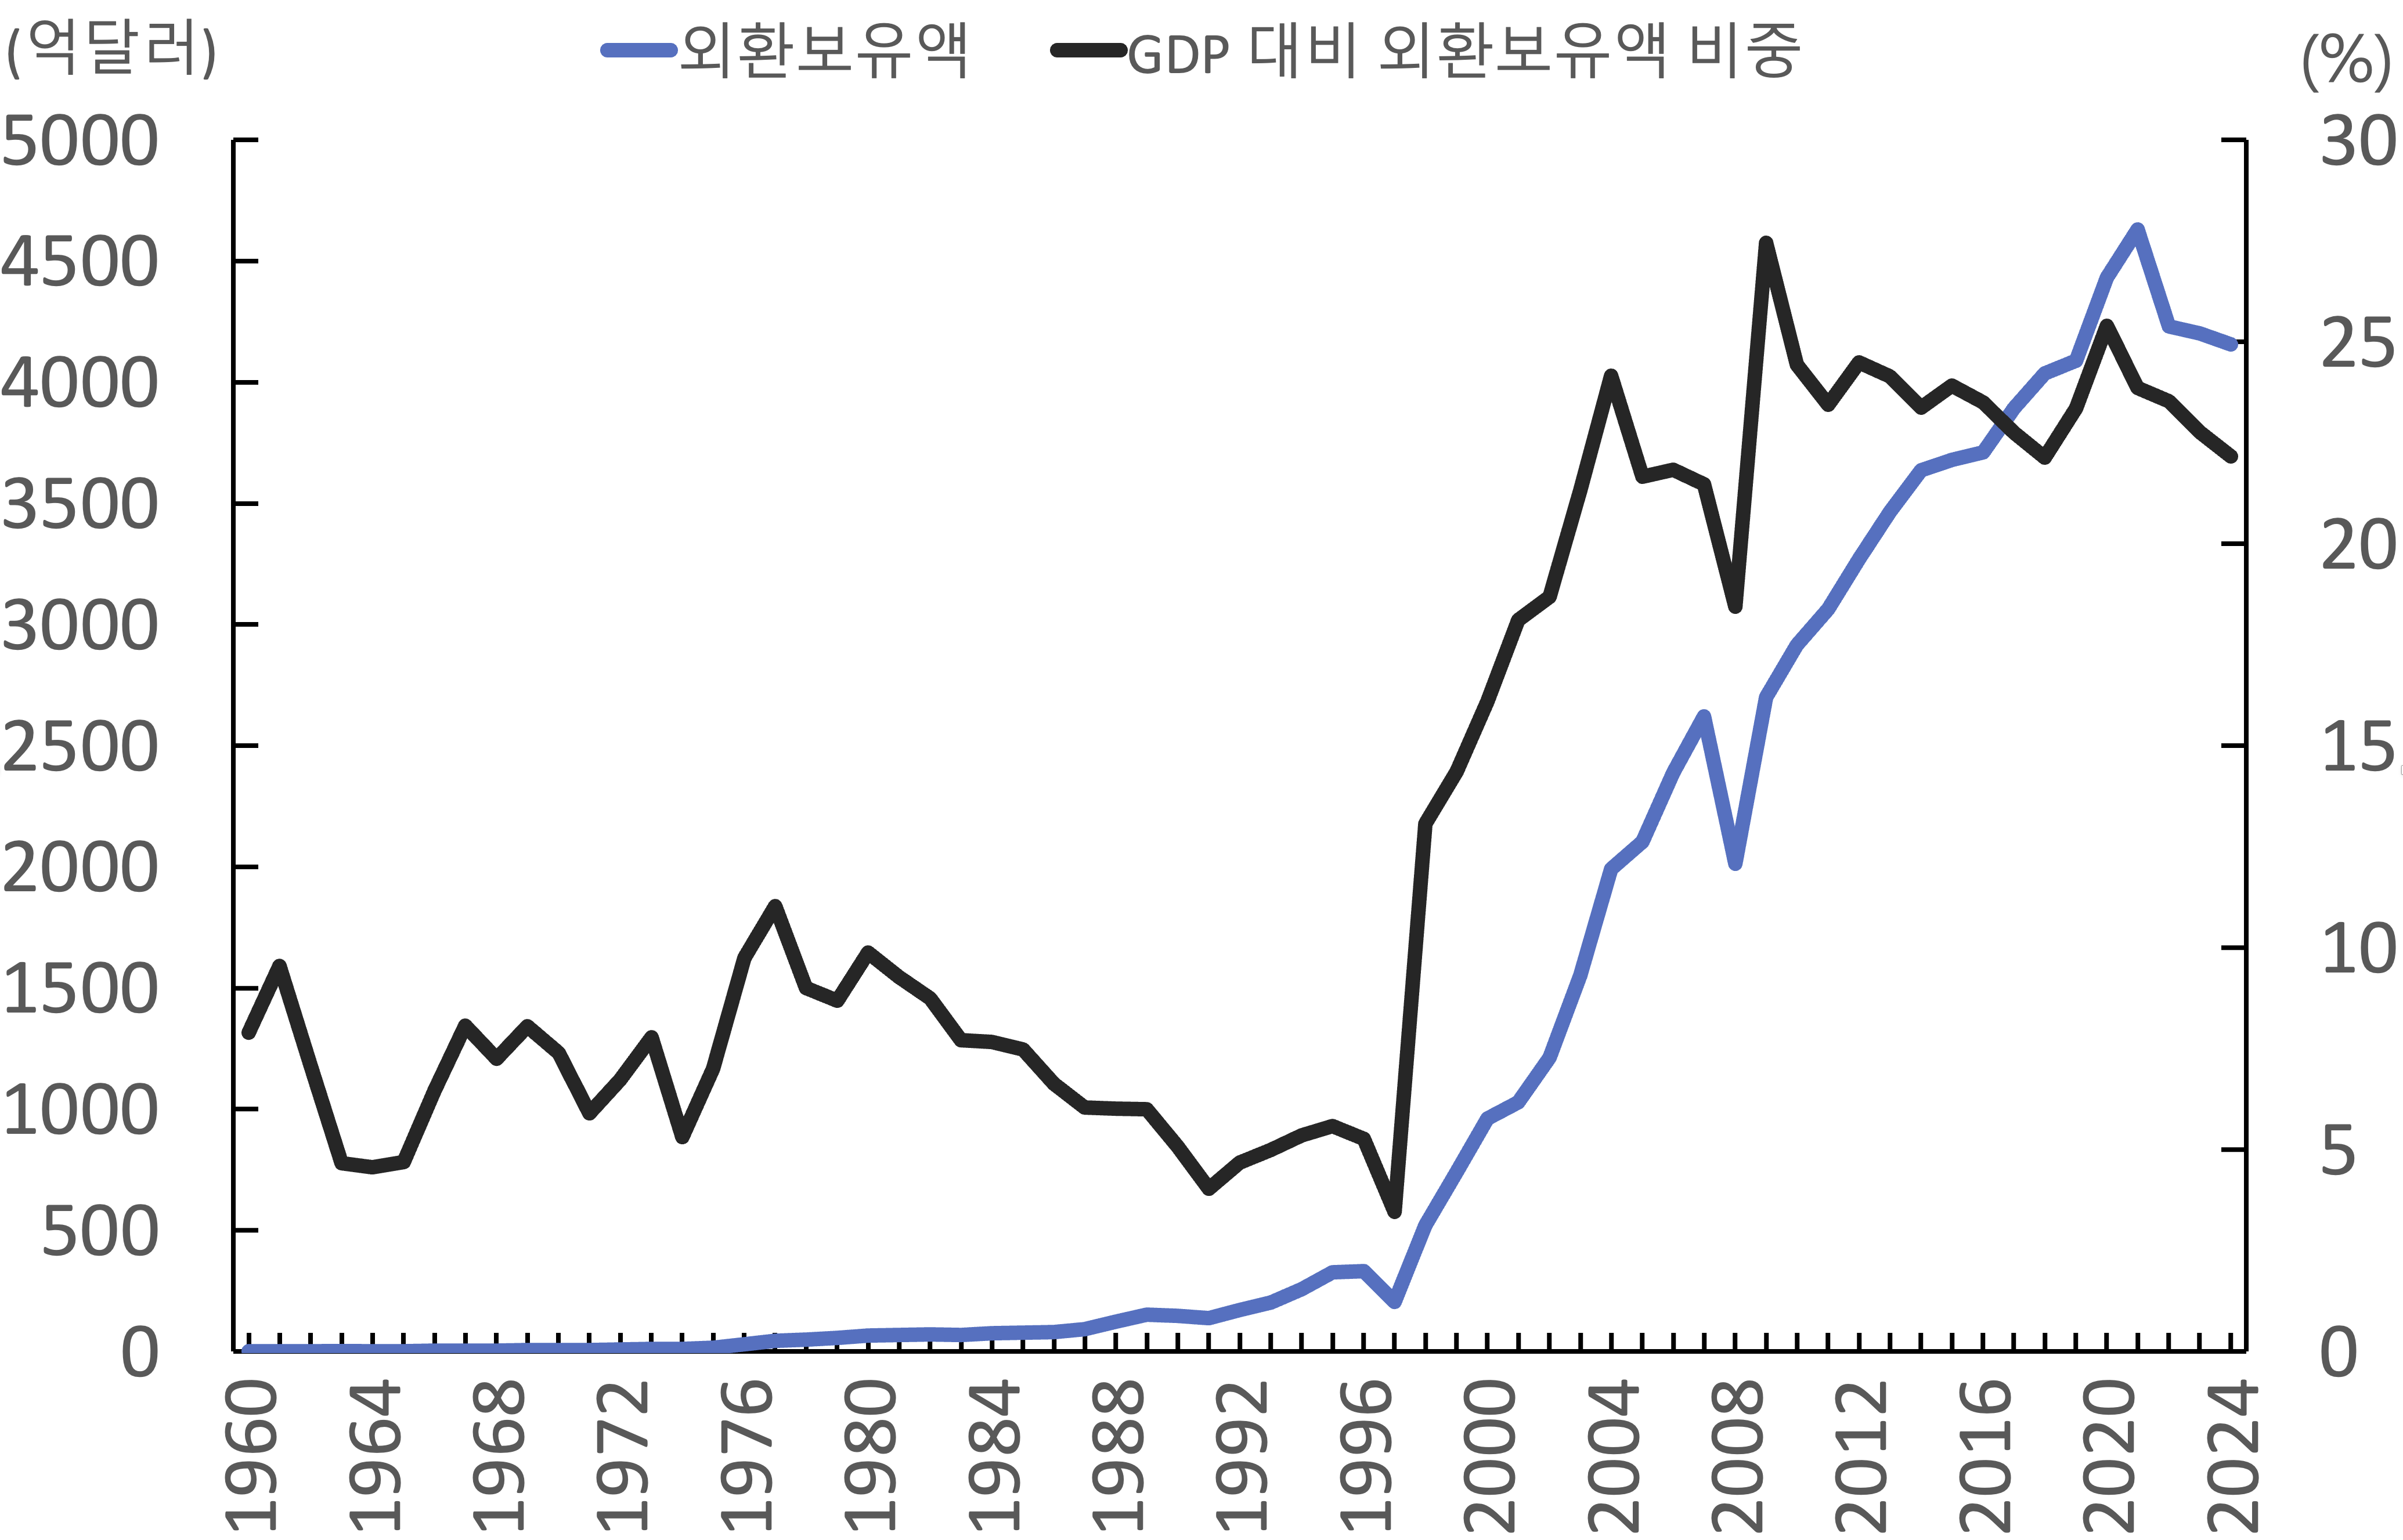
\includegraphics[width=.8\textwidth]{pic/fig_econ_08.png}
        \end{figure}
        \begin{itemize}[<+->]
            \item 초기에는 외환보유에 소극적이었지만, 외환위기 이후 보유액을 크게 늘려 위기 대응력을 확보했다.
        \end{itemize}
    \end{column}
    \begin{column}{.5\textwidth}
        \begin{figure}
            \centering
            \only<1|handout:0>{\transparent{0.3}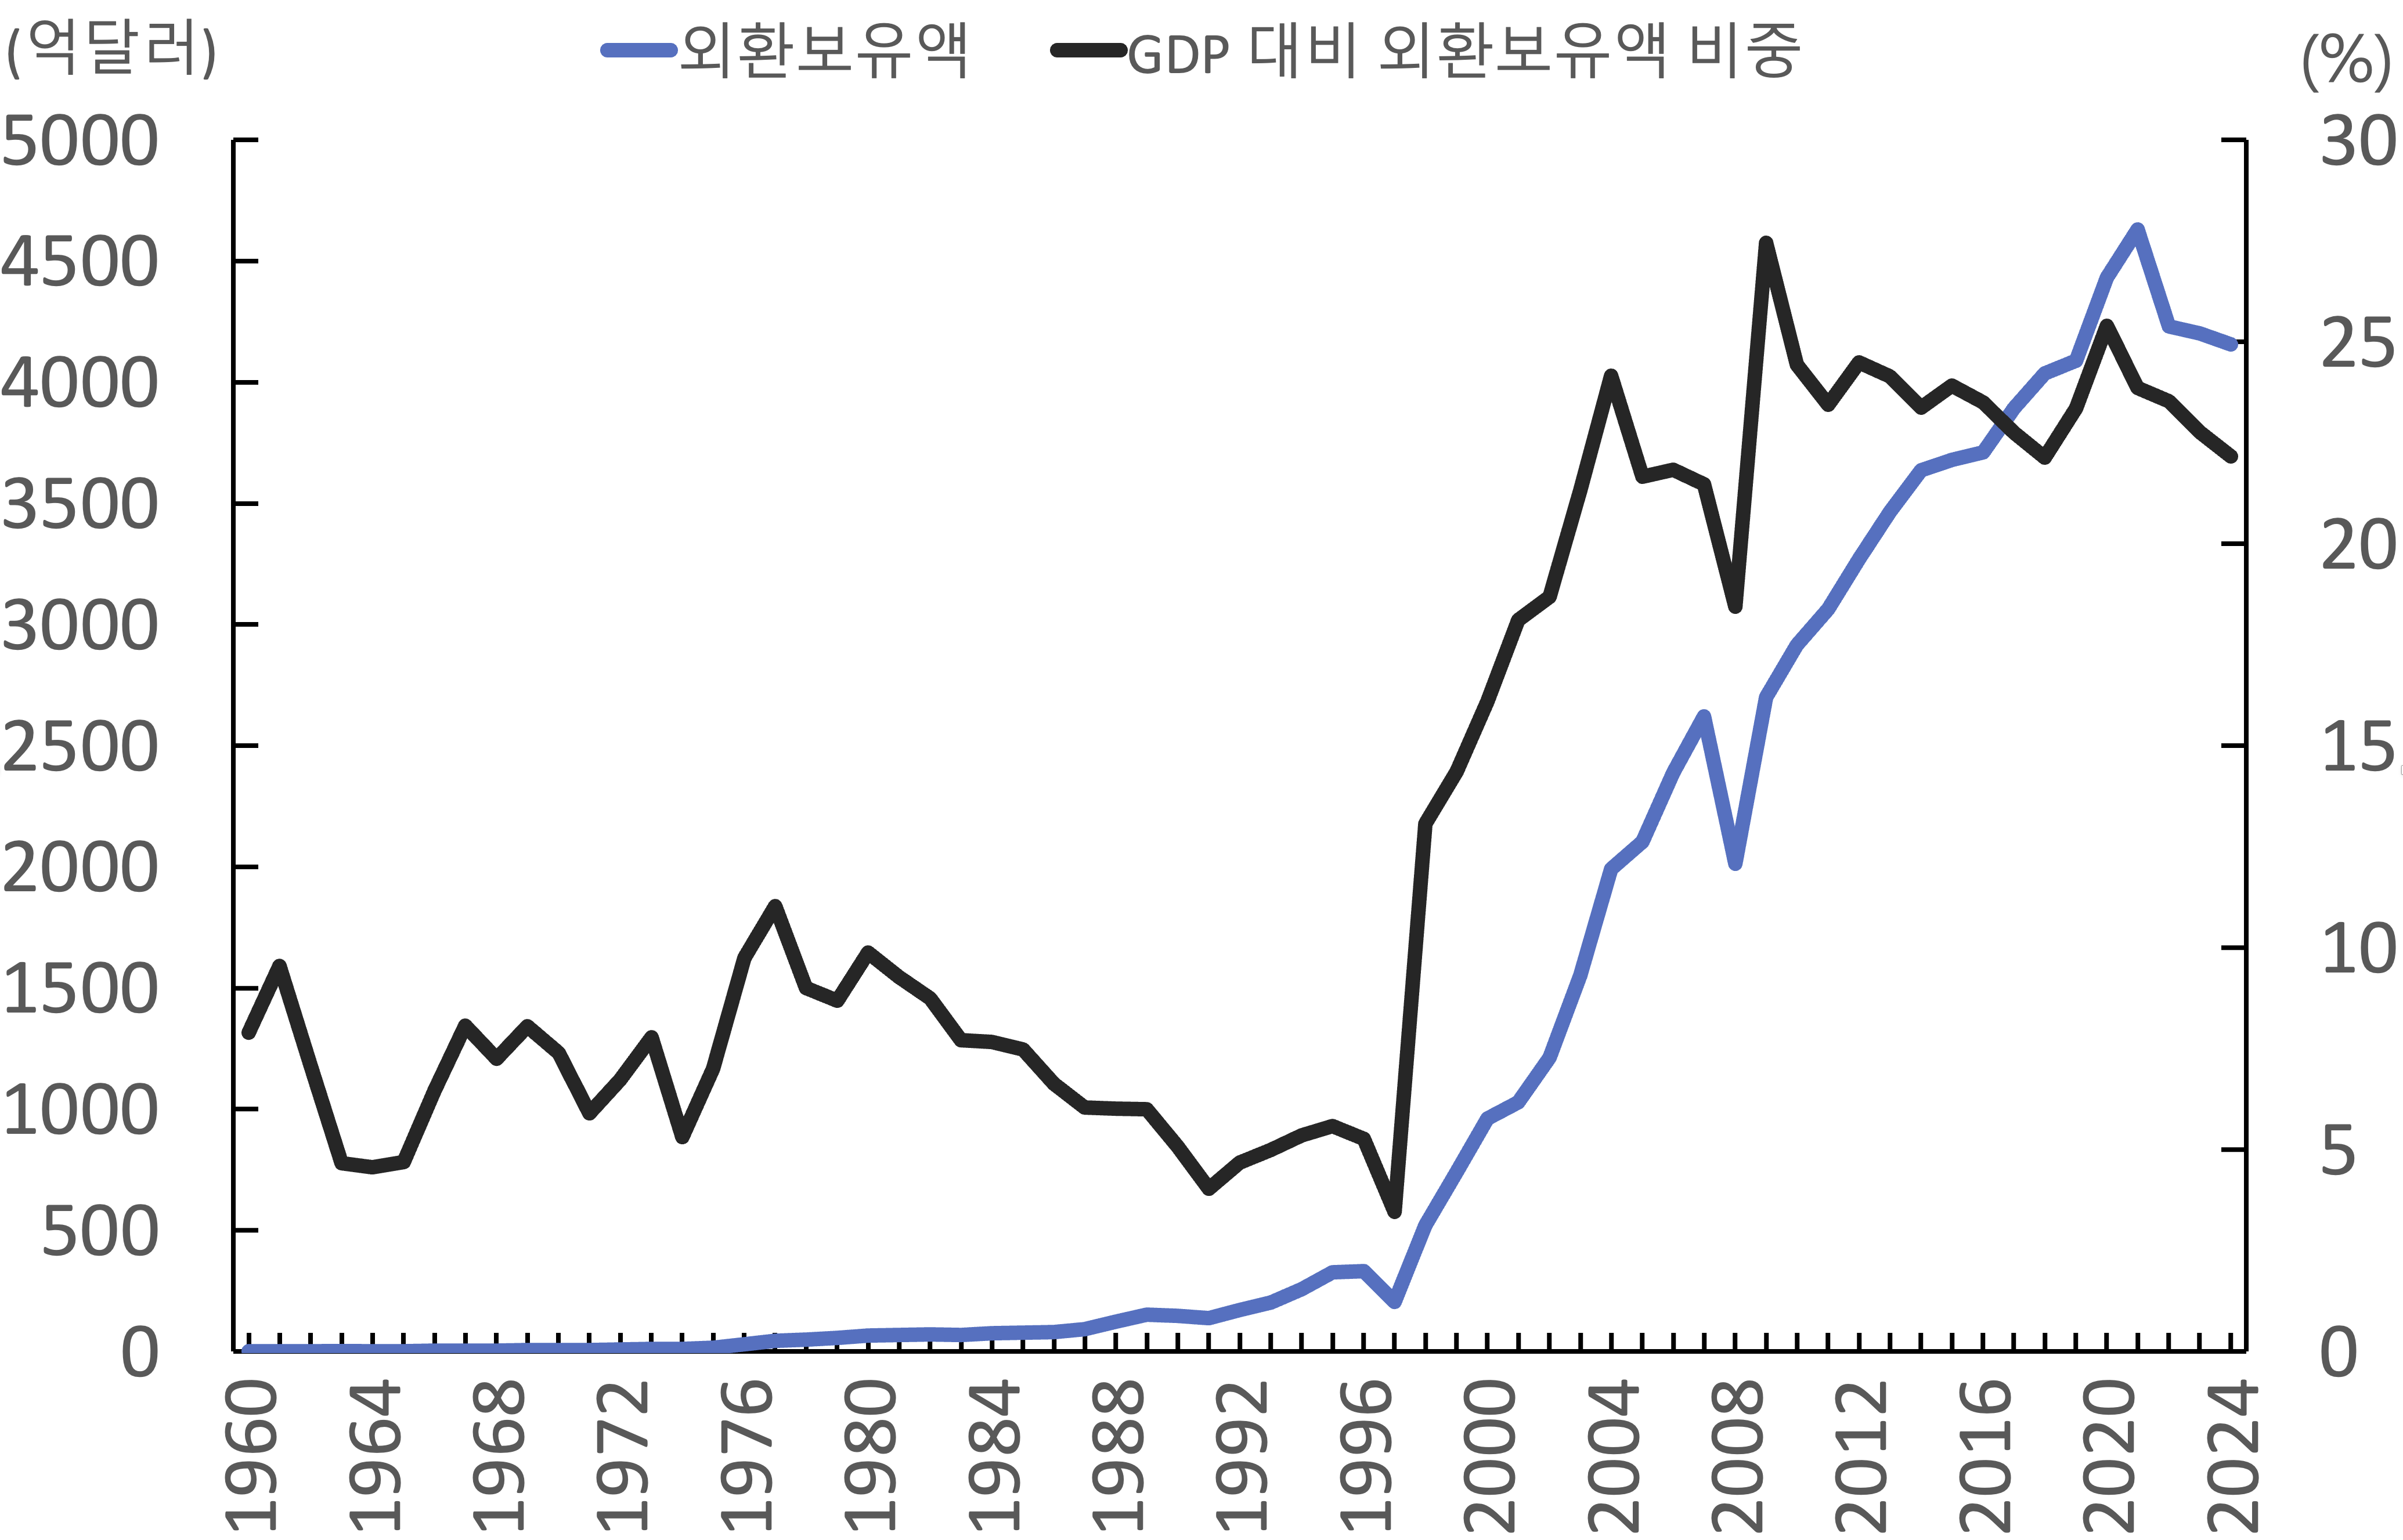
\includegraphics[width=.8\textwidth]{pic/fig_econ_08.png}} % 첫 번째 슬라이드: 투명하게 표시
            \only<2>{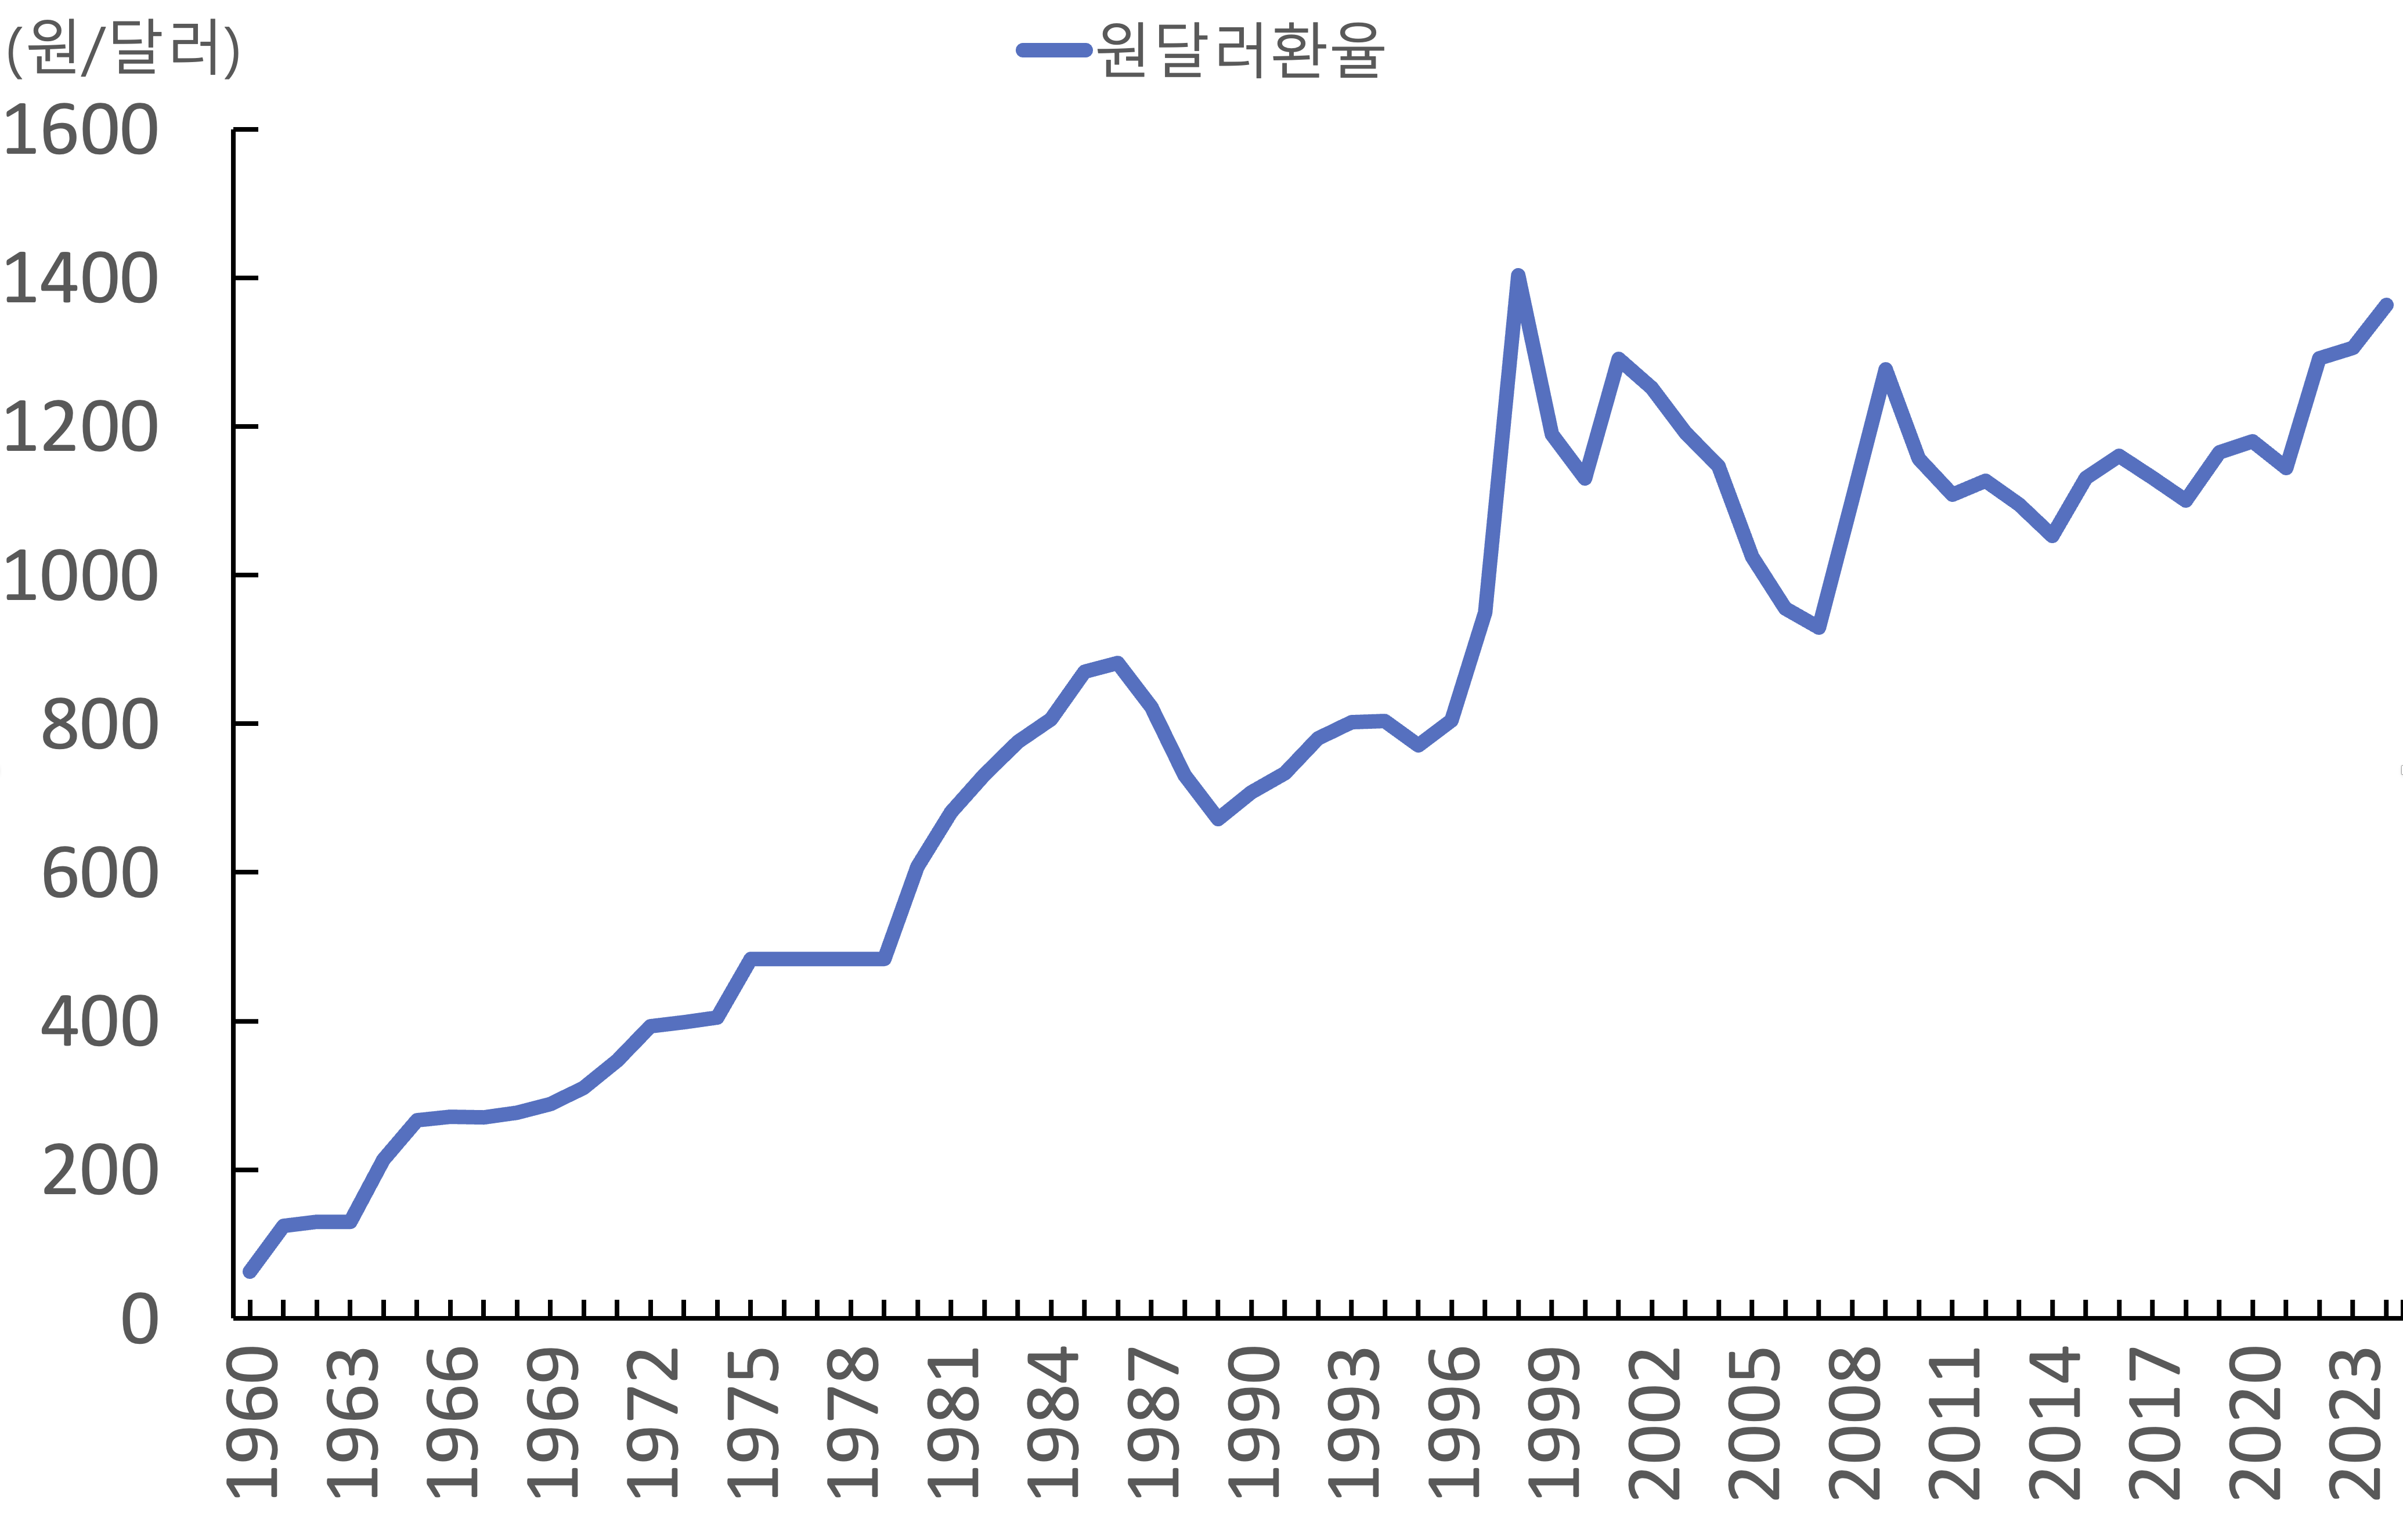
\includegraphics[width=.8\textwidth]{pic/fig_econ_09.png}} % 두 번째 슬라이드: 선명하게 표시
            \\
        \end{figure}
        \begin{itemize}[<+->]
            \item 1달러=50원의 고정환율제에서 출발해 외환위기를 거치며 환율을 시장이 결정하는 구조로 전환했다.
        \end{itemize}
    \end{column}
\end{columns}
\end{frame}

\subsection{정부지출}
\begin{frame}[<+->]
\frametitle{개발재정에서 복지재정으로 전환을 이루다.}
    \begin{figure}
        \centering
        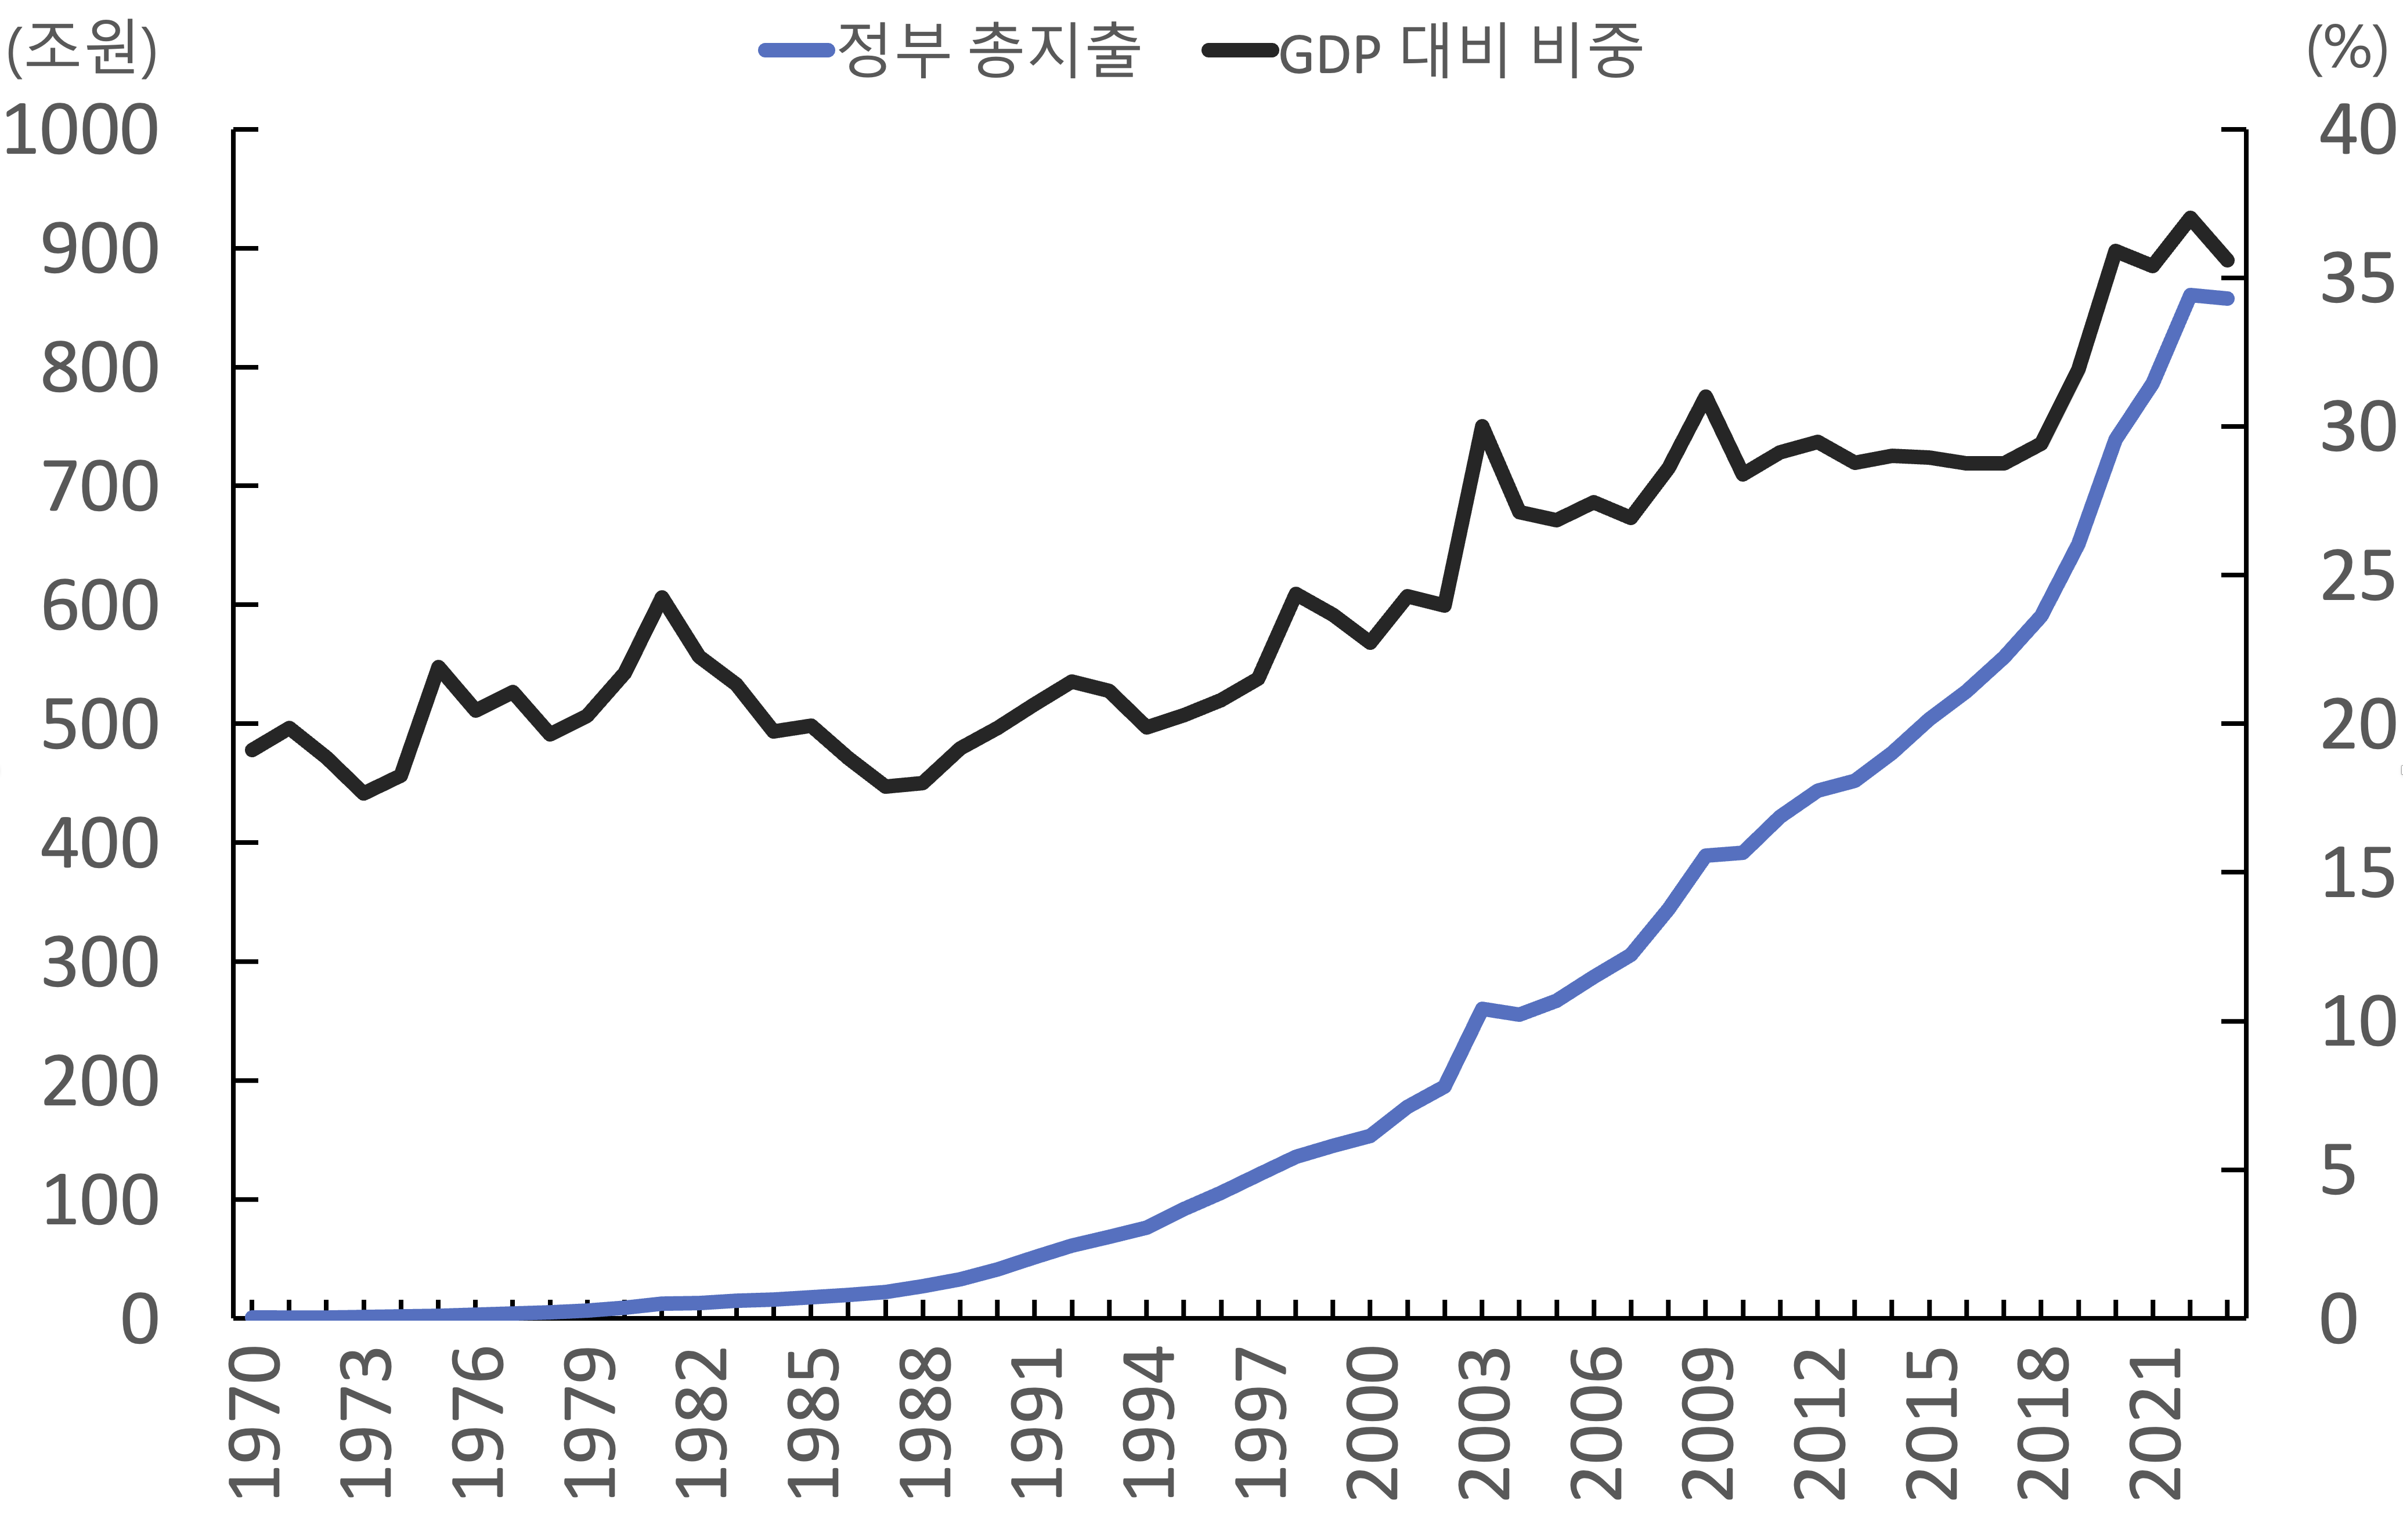
\includegraphics[width=.5\textwidth]{pic/fig_econ_10.png}
    \end{figure}
    \begin{itemize}
        \item 산업화 지원 중심이던 정부 재정은 복지·고용 안정 중심으로 확대되며 국민 삶을 지탱하는 재정으로 변했다.
    \end{itemize}
\end{frame}

\begin{frame}[<+->]
\frametitle{국방과 산업 대신 복지와 사회보호가 국가 재정의 중심이 되다.}
    \begin{figure}
        \centering
        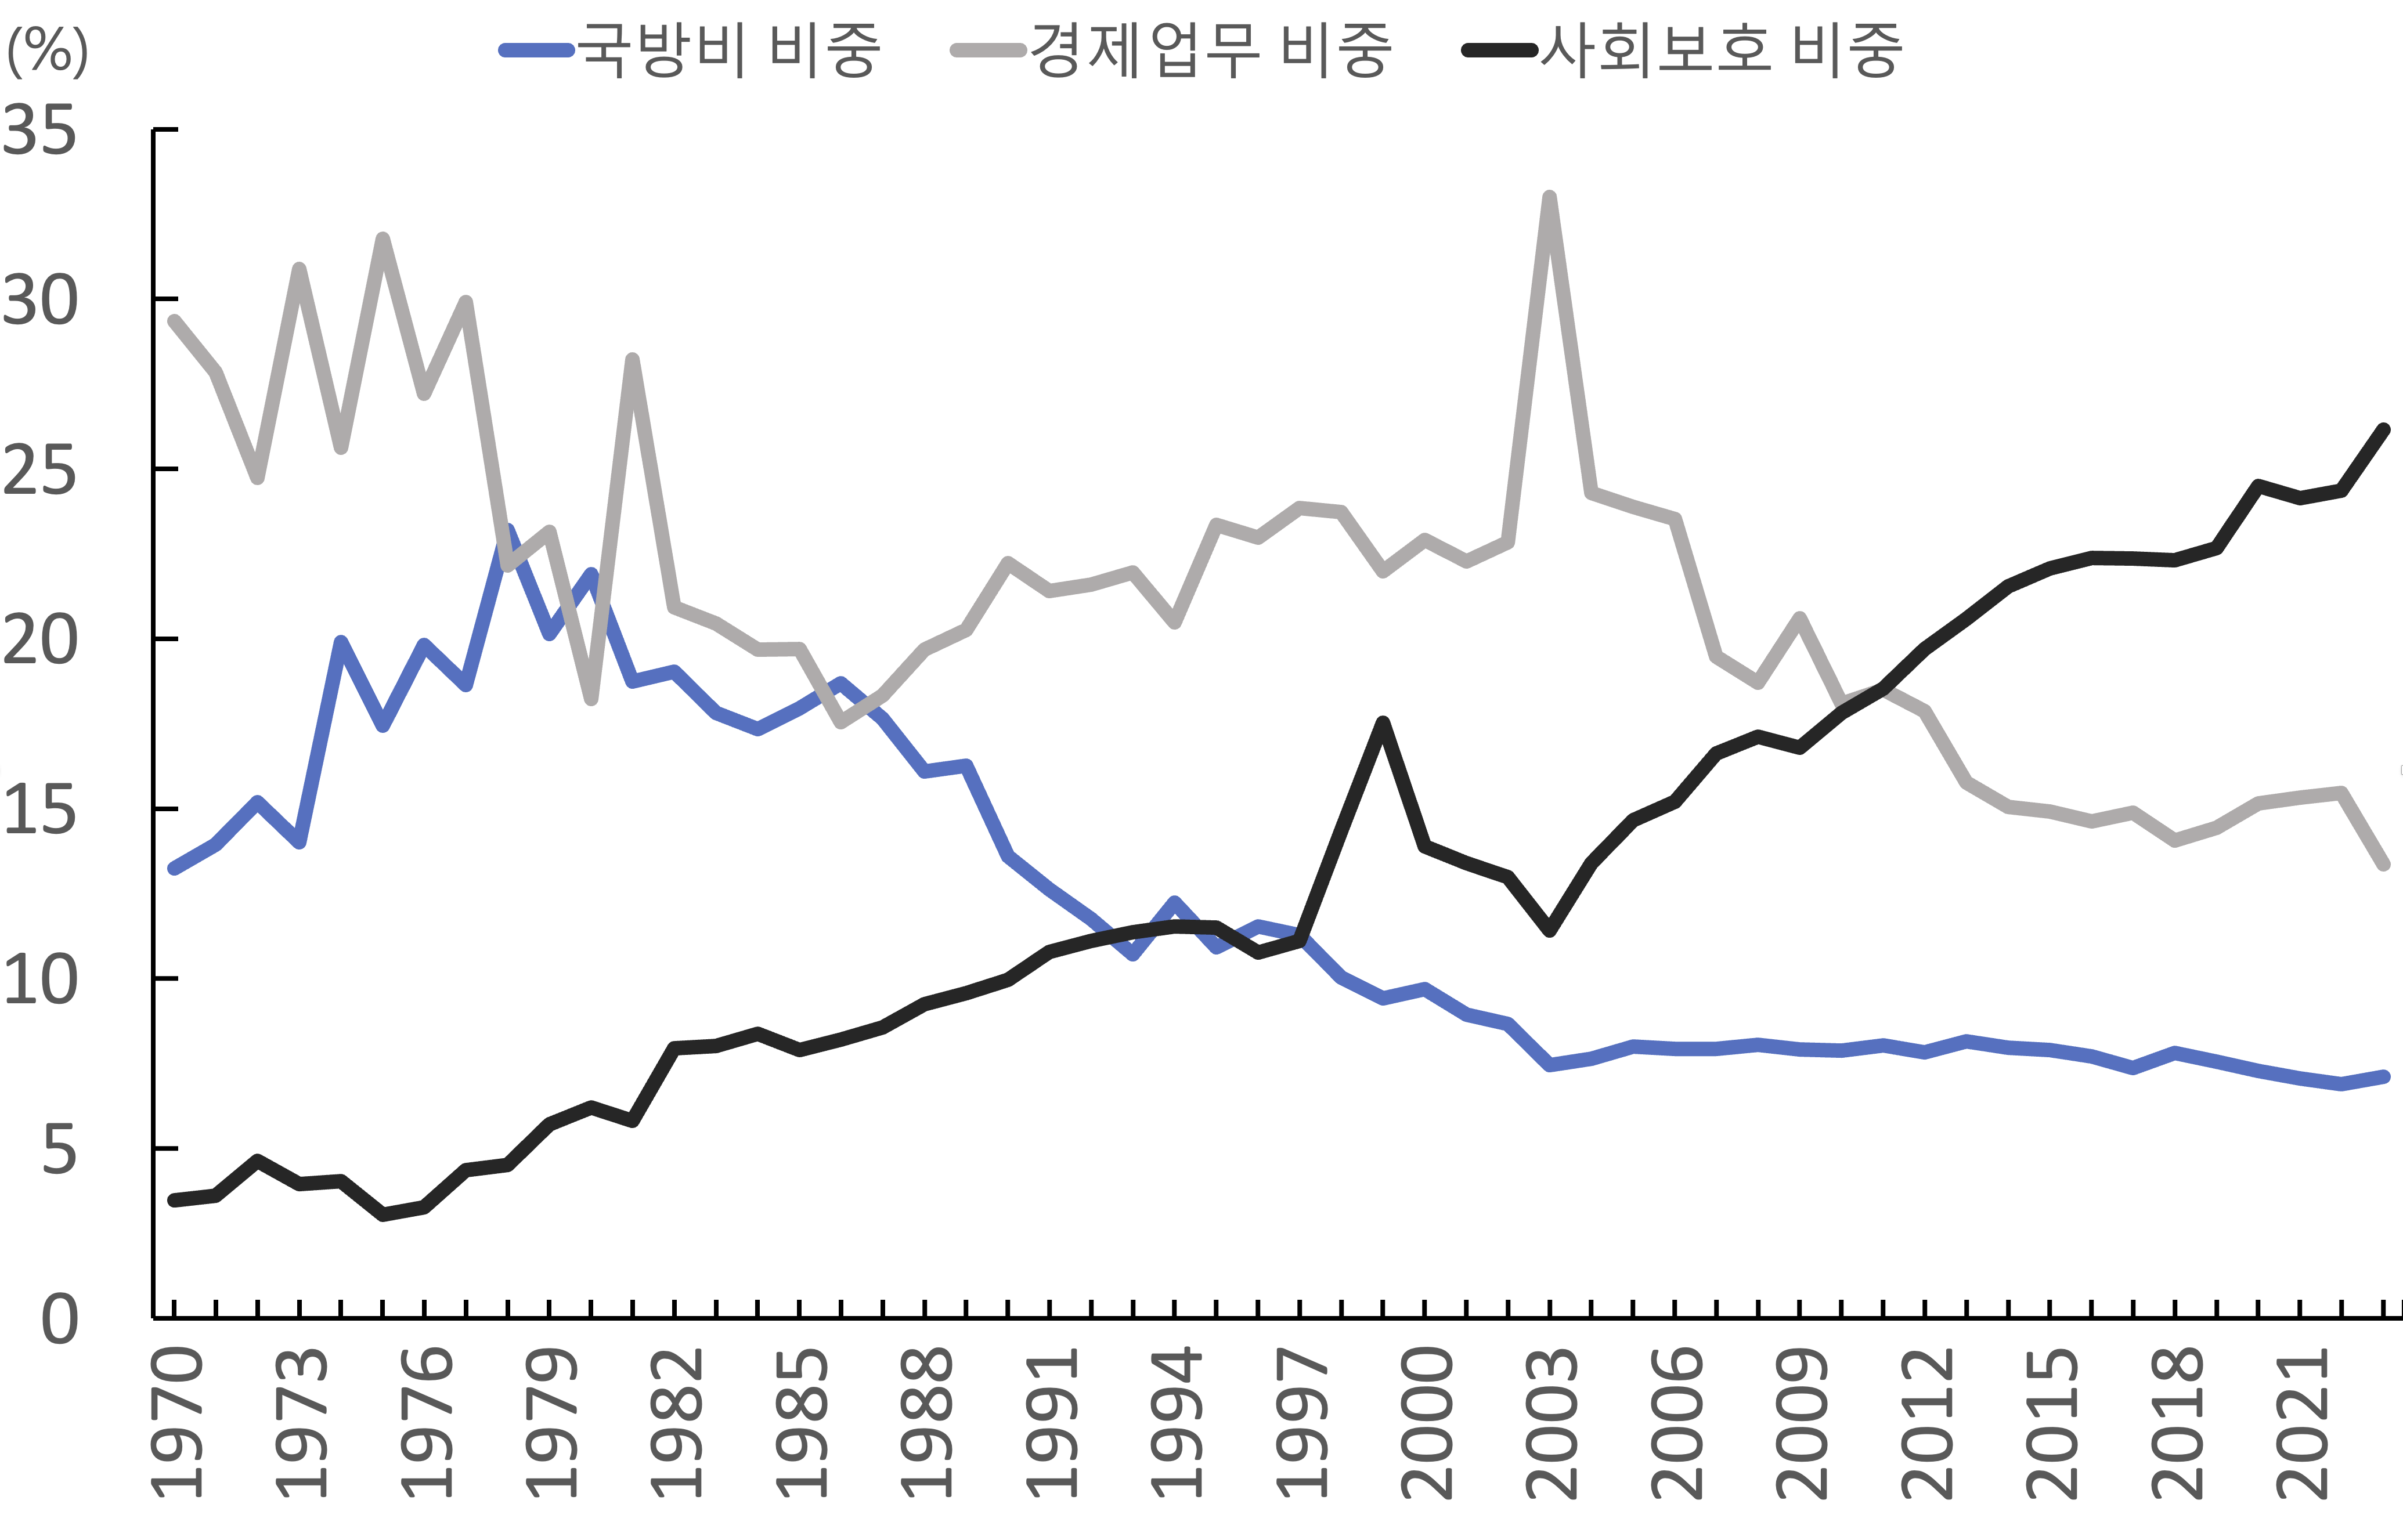
\includegraphics[width=.5\textwidth]{pic/fig_econ_11.png}
    \end{figure}
    \begin{itemize}
        \item  국방·산업 지출의 비중은 줄고, 복지와 사회보호가 가장 큰 재정 항목으로 부상했다.
    \end{itemize}
\end{frame}

\begin{frame}[<+->]
\frametitle{세금과 사회보험료를 함께 늘리며 복지국가로 나아가다.}
    \begin{figure}
        \centering
        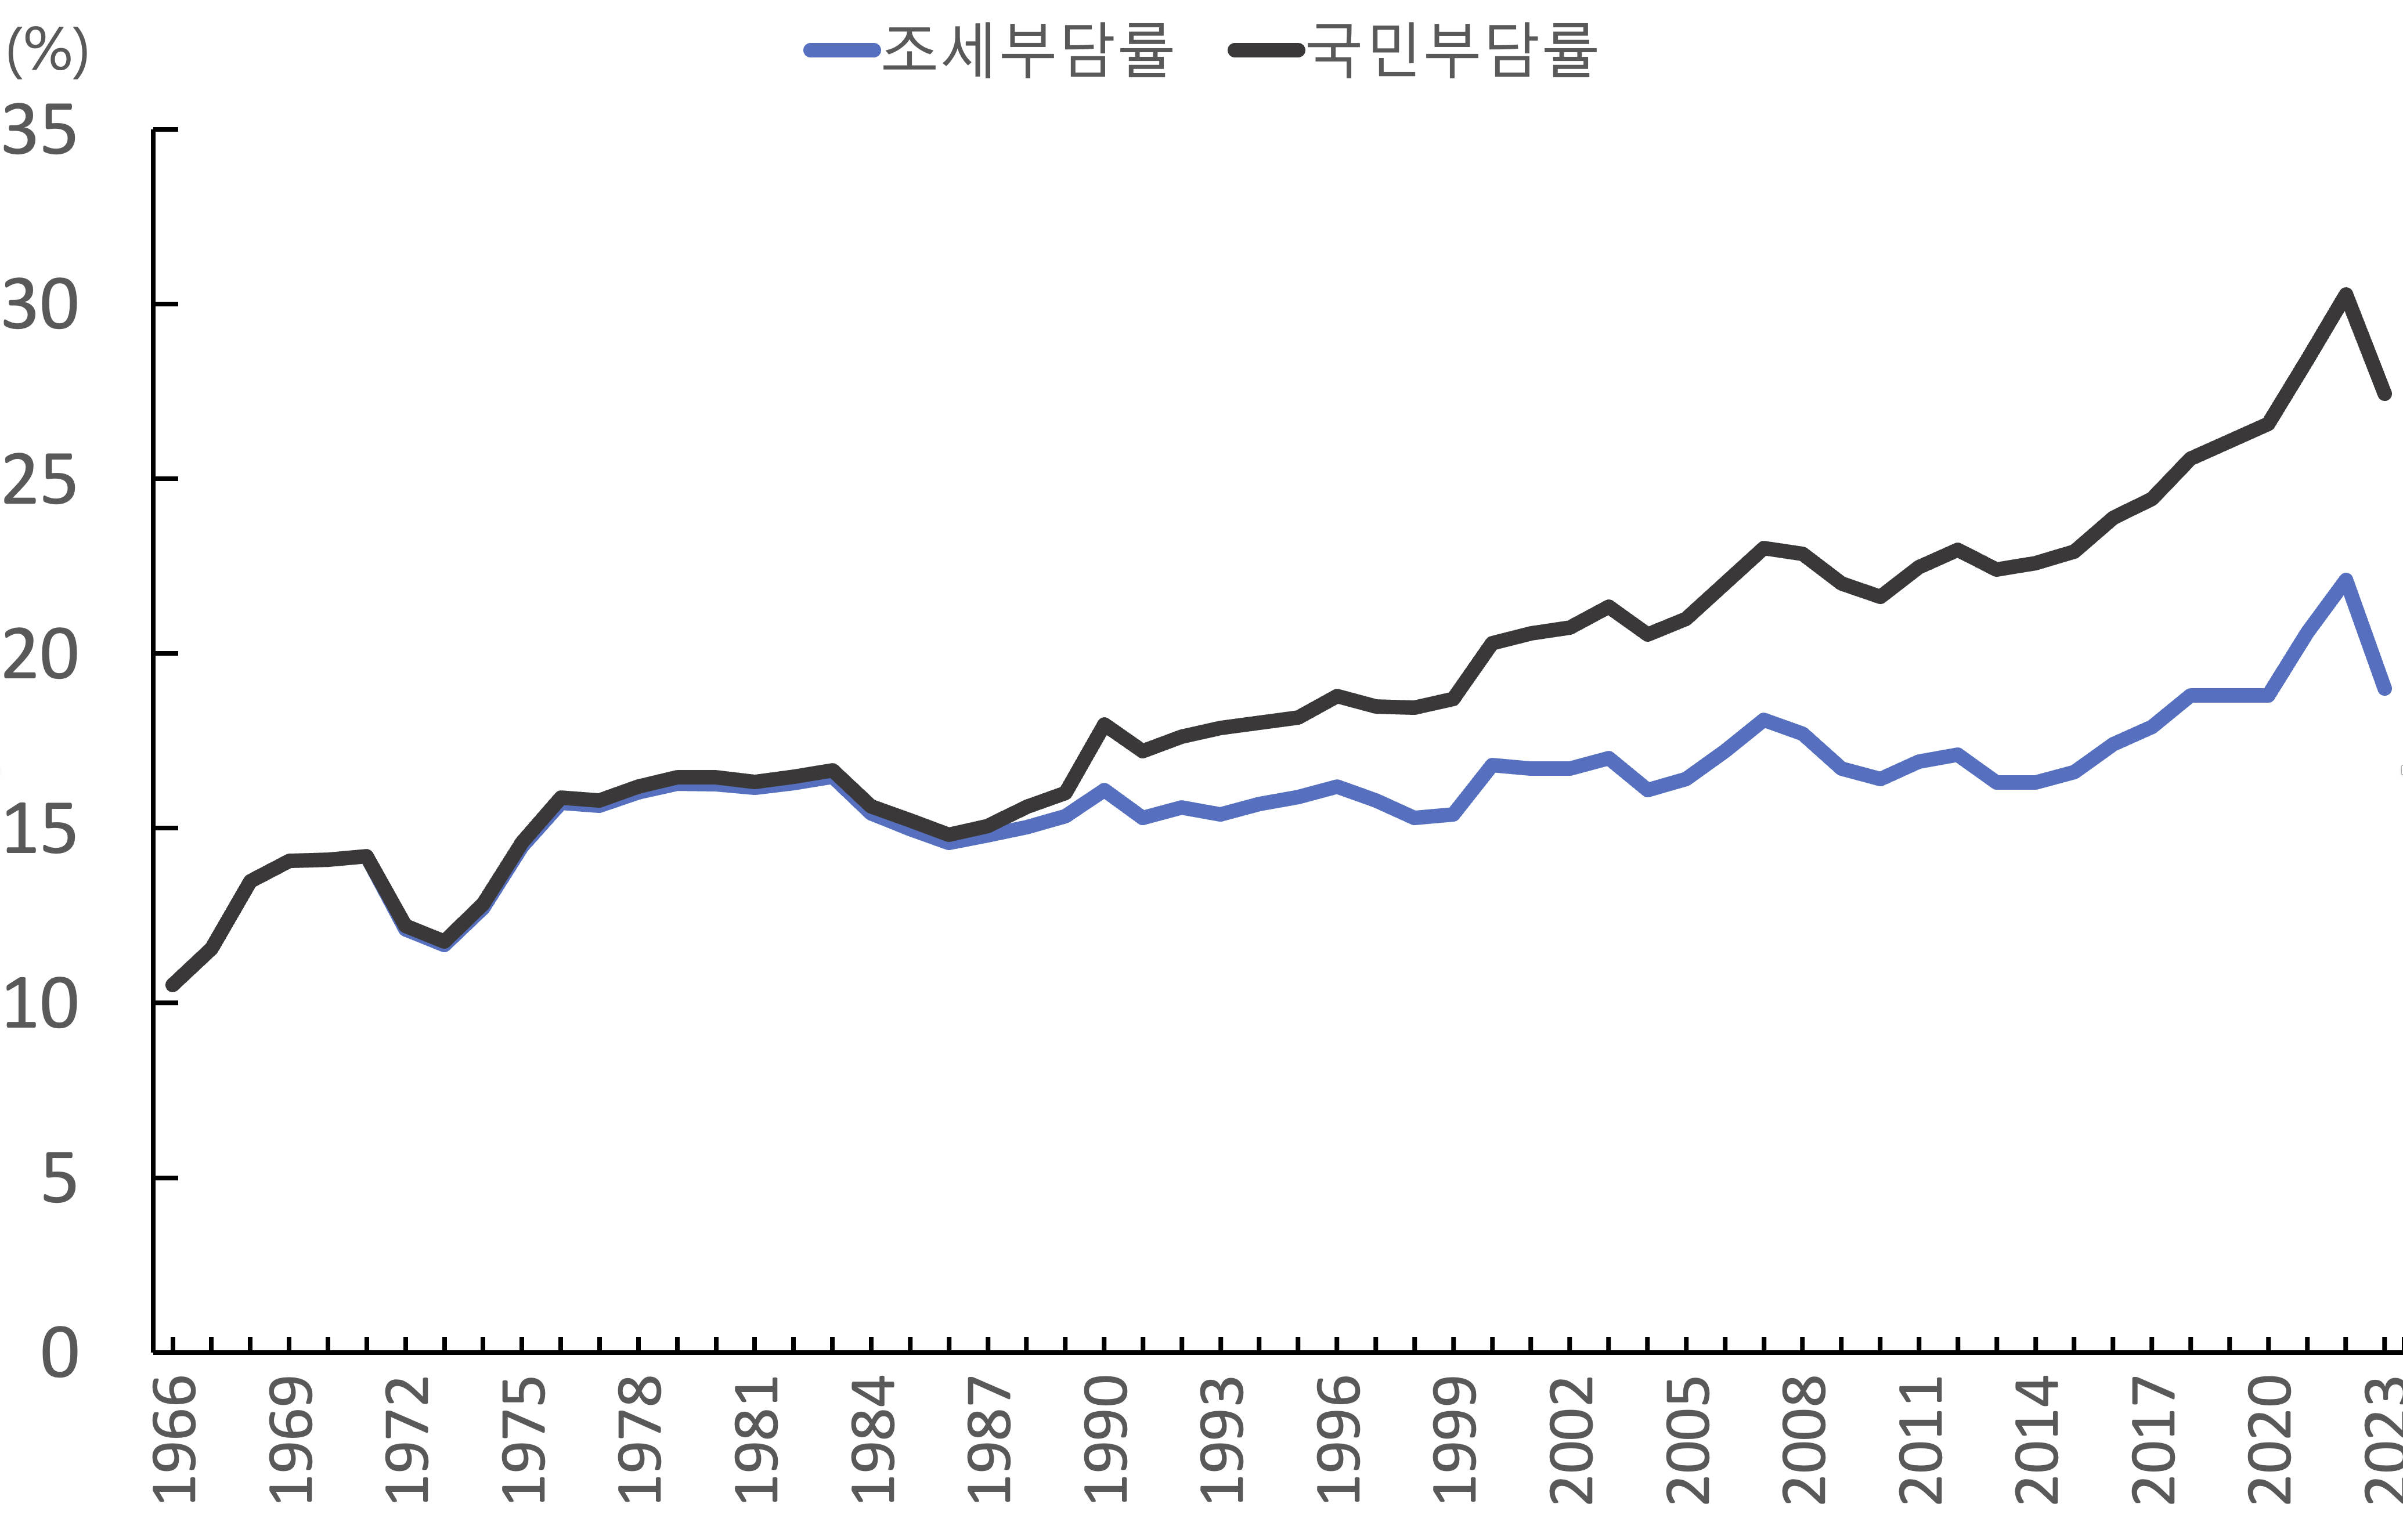
\includegraphics[width=.5\textwidth]{pic/fig_econ_12.png}
    \end{figure}
    \begin{itemize}
        \item 한국은 조세와 사회보험료가 꾸준히 증가하며 복지국가로 가는 길을 본격적으로 걸어갔다.
    \end{itemize}
\end{frame}

\section{소득•지출 분야}
\subsection{소득}
\begin{frame}[<+->]
\frametitle{가구 소득이 절대 빈곤에서 선진국 수준으로 도약했다.}
    \begin{figure}
        \centering
        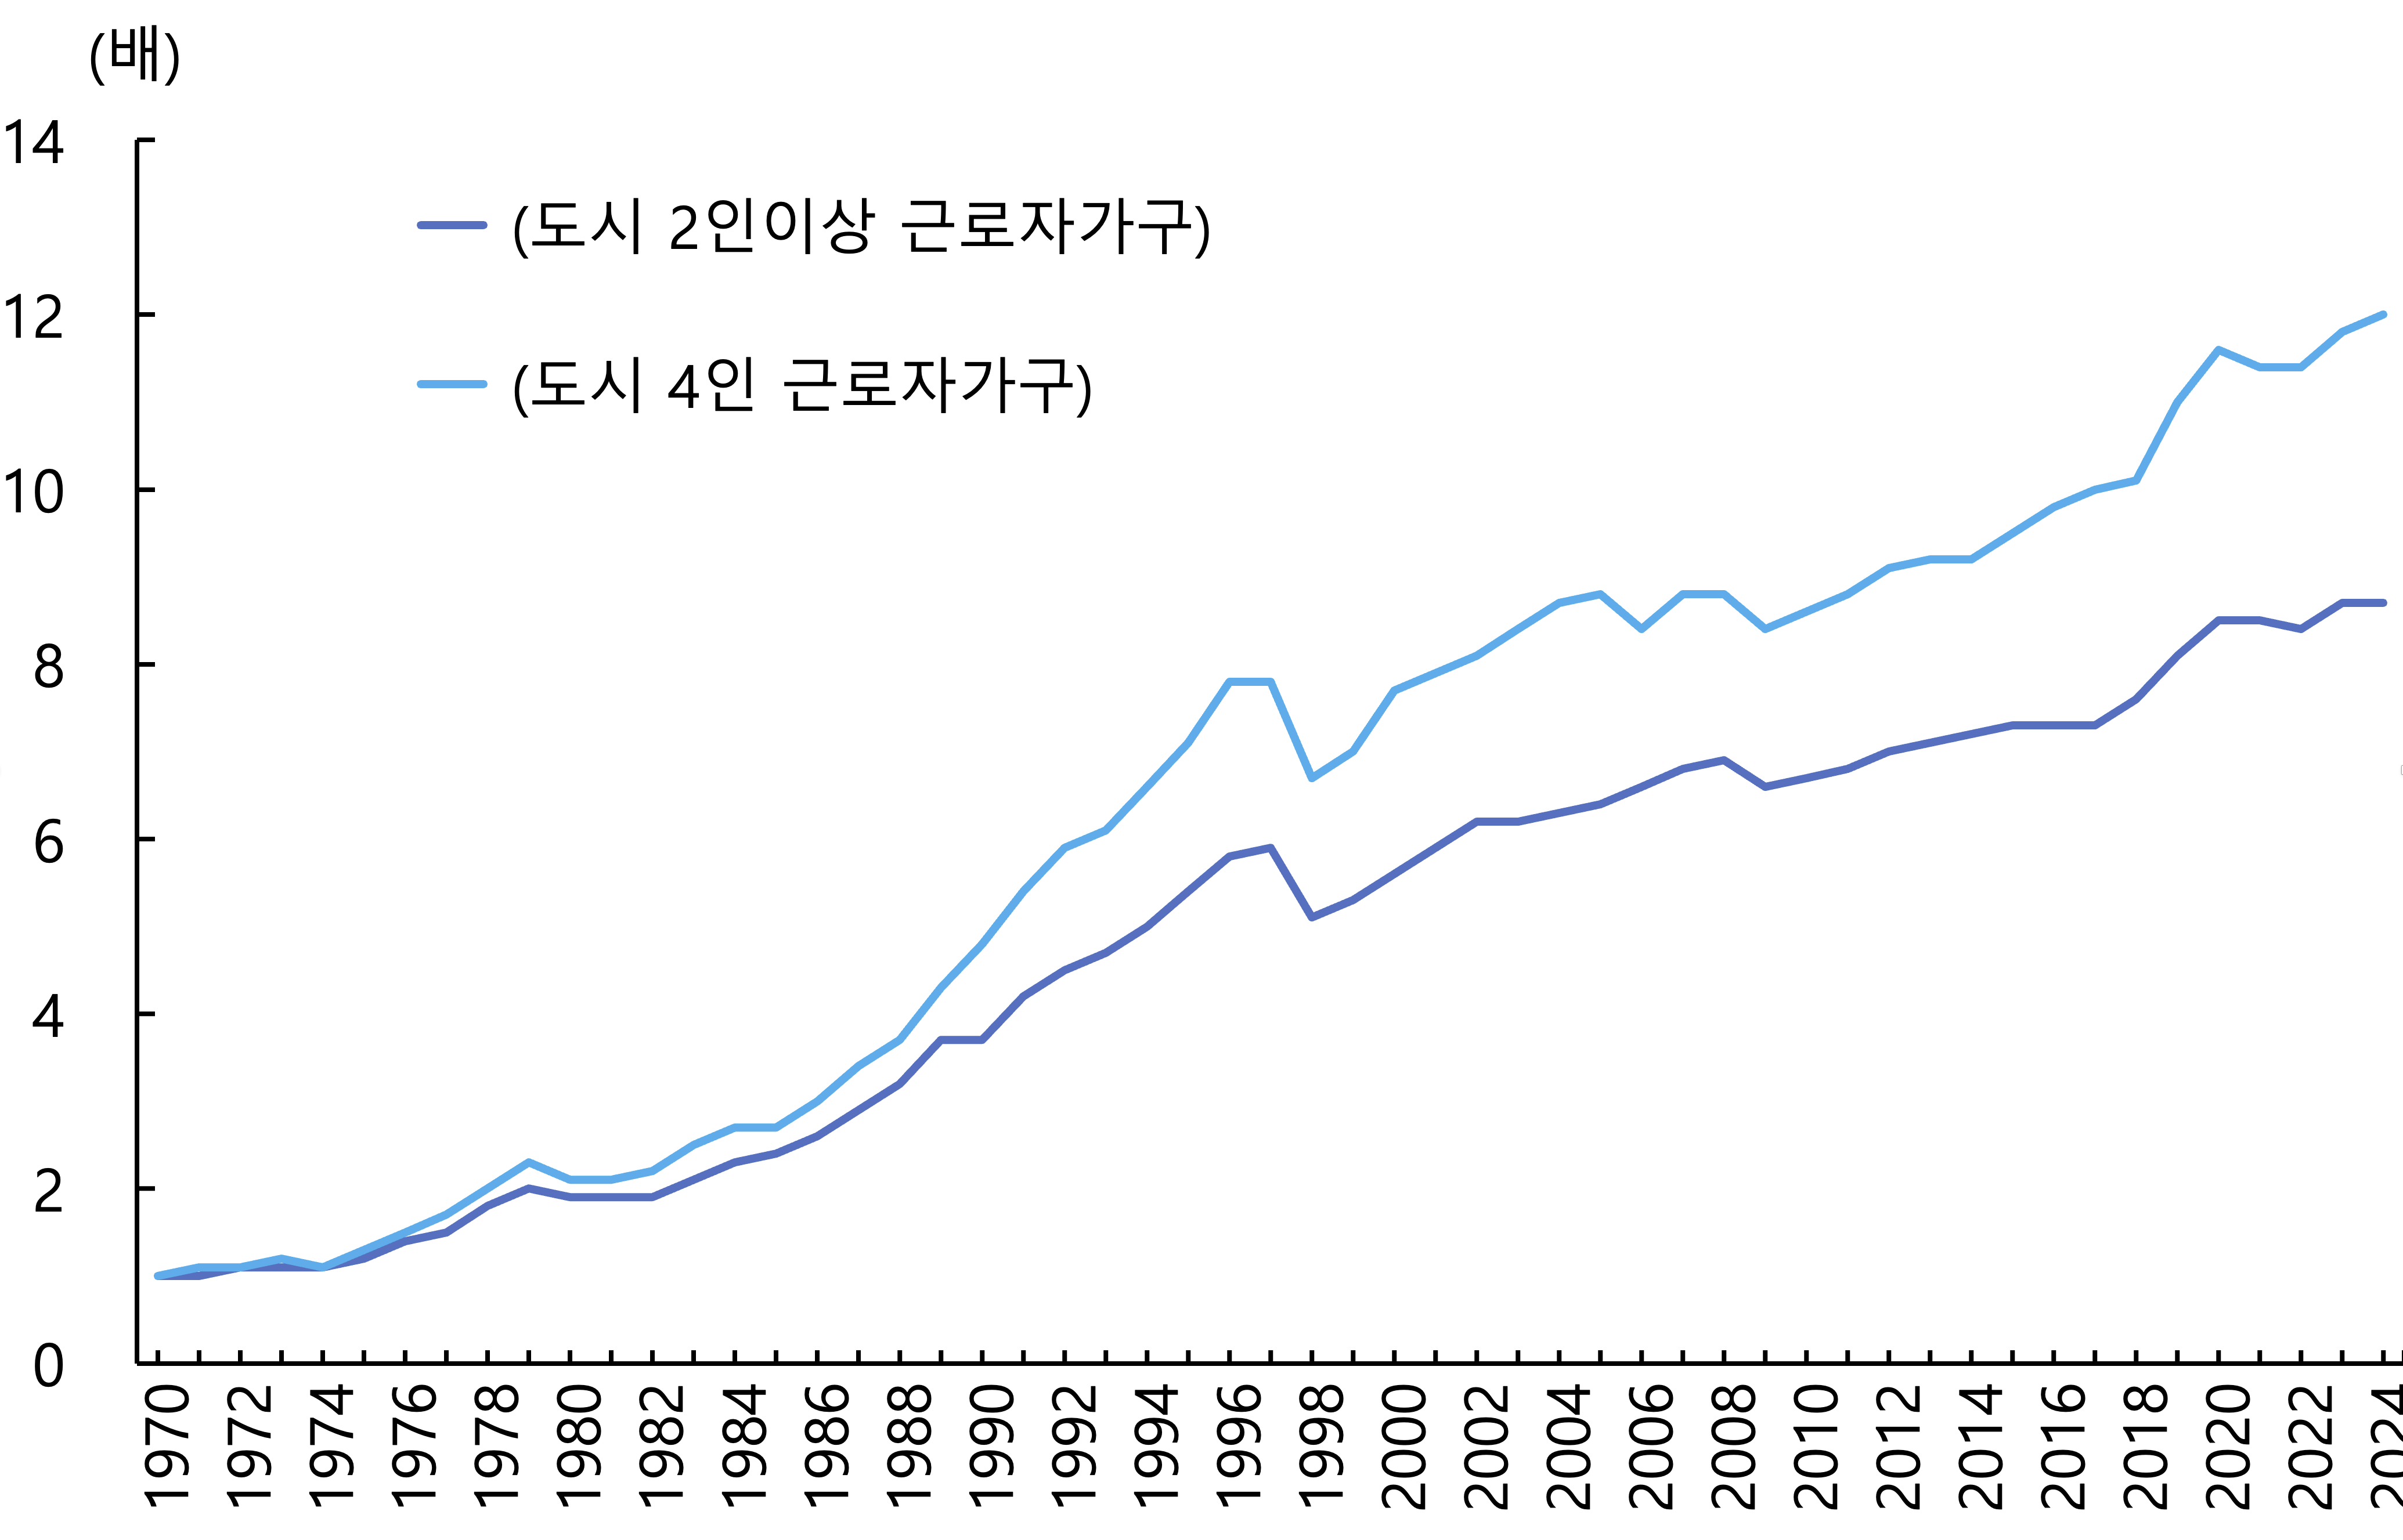
\includegraphics[width=.5\textwidth]{pic/fig_ineq_01.png}
    \end{figure}
    \begin{itemize}
        \item 1970년 월 56만원이던 (실질 처분가능)가구 소득은 산업화와 경제 성장의 힘으로 2024년까지 10배 이상 실질적으로 증가하며 세계 선진국 수준에 다가섰다.
    \end{itemize}
\end{frame}

\subsection{물가}
\begin{frame}[<+->]
\frametitle{물가 안정이 생활수준 향상의 토대가 되었다.}
    \begin{figure}
        \centering
        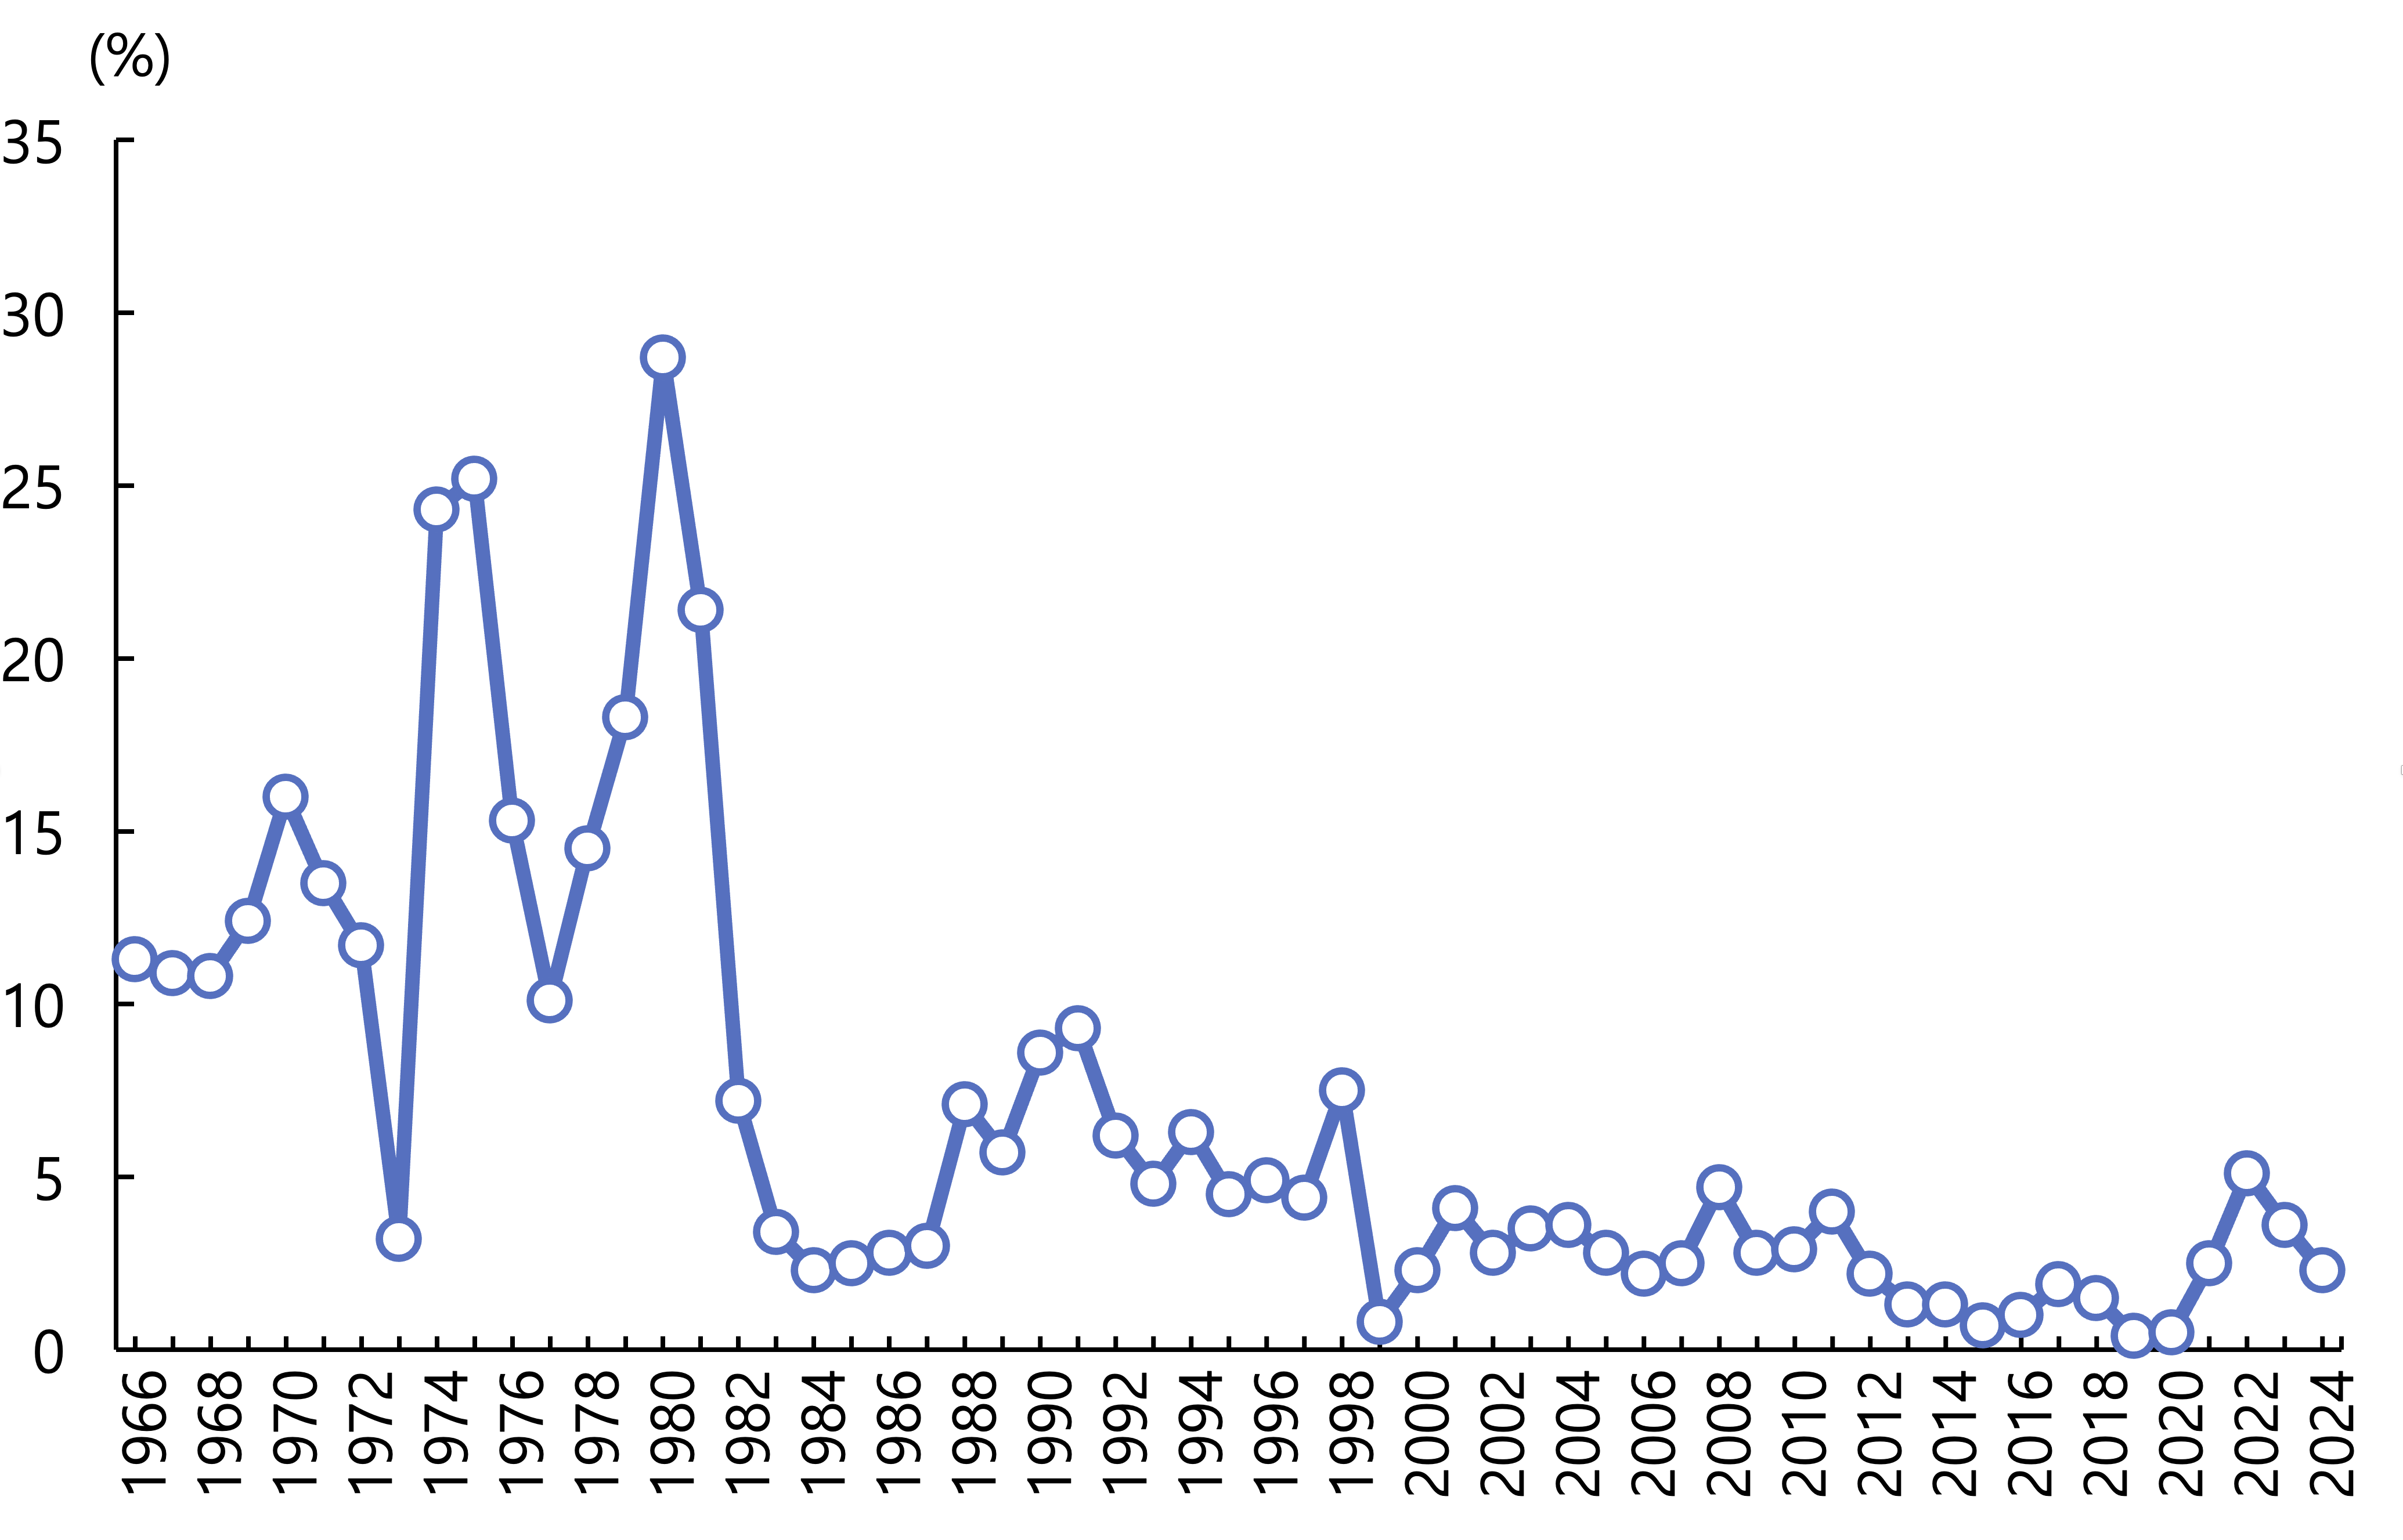
\includegraphics[width=.5\textwidth]{pic/fig_ineq_02.png}
    \end{figure}
    \begin{itemize}
        \item 1970년대까지 두 자릿수였던 물가상승률은 1980년대 이후 안정되며 소득 증가가 실질 생활 개선으로 이어질 수 있었다.
    \end{itemize}
\end{frame}

\begin{frame}[<+->]
\frametitle{가구 지출이 생활수준 향상과 소비문화 확산을 이끌었다.}
    \begin{figure}
        \centering
        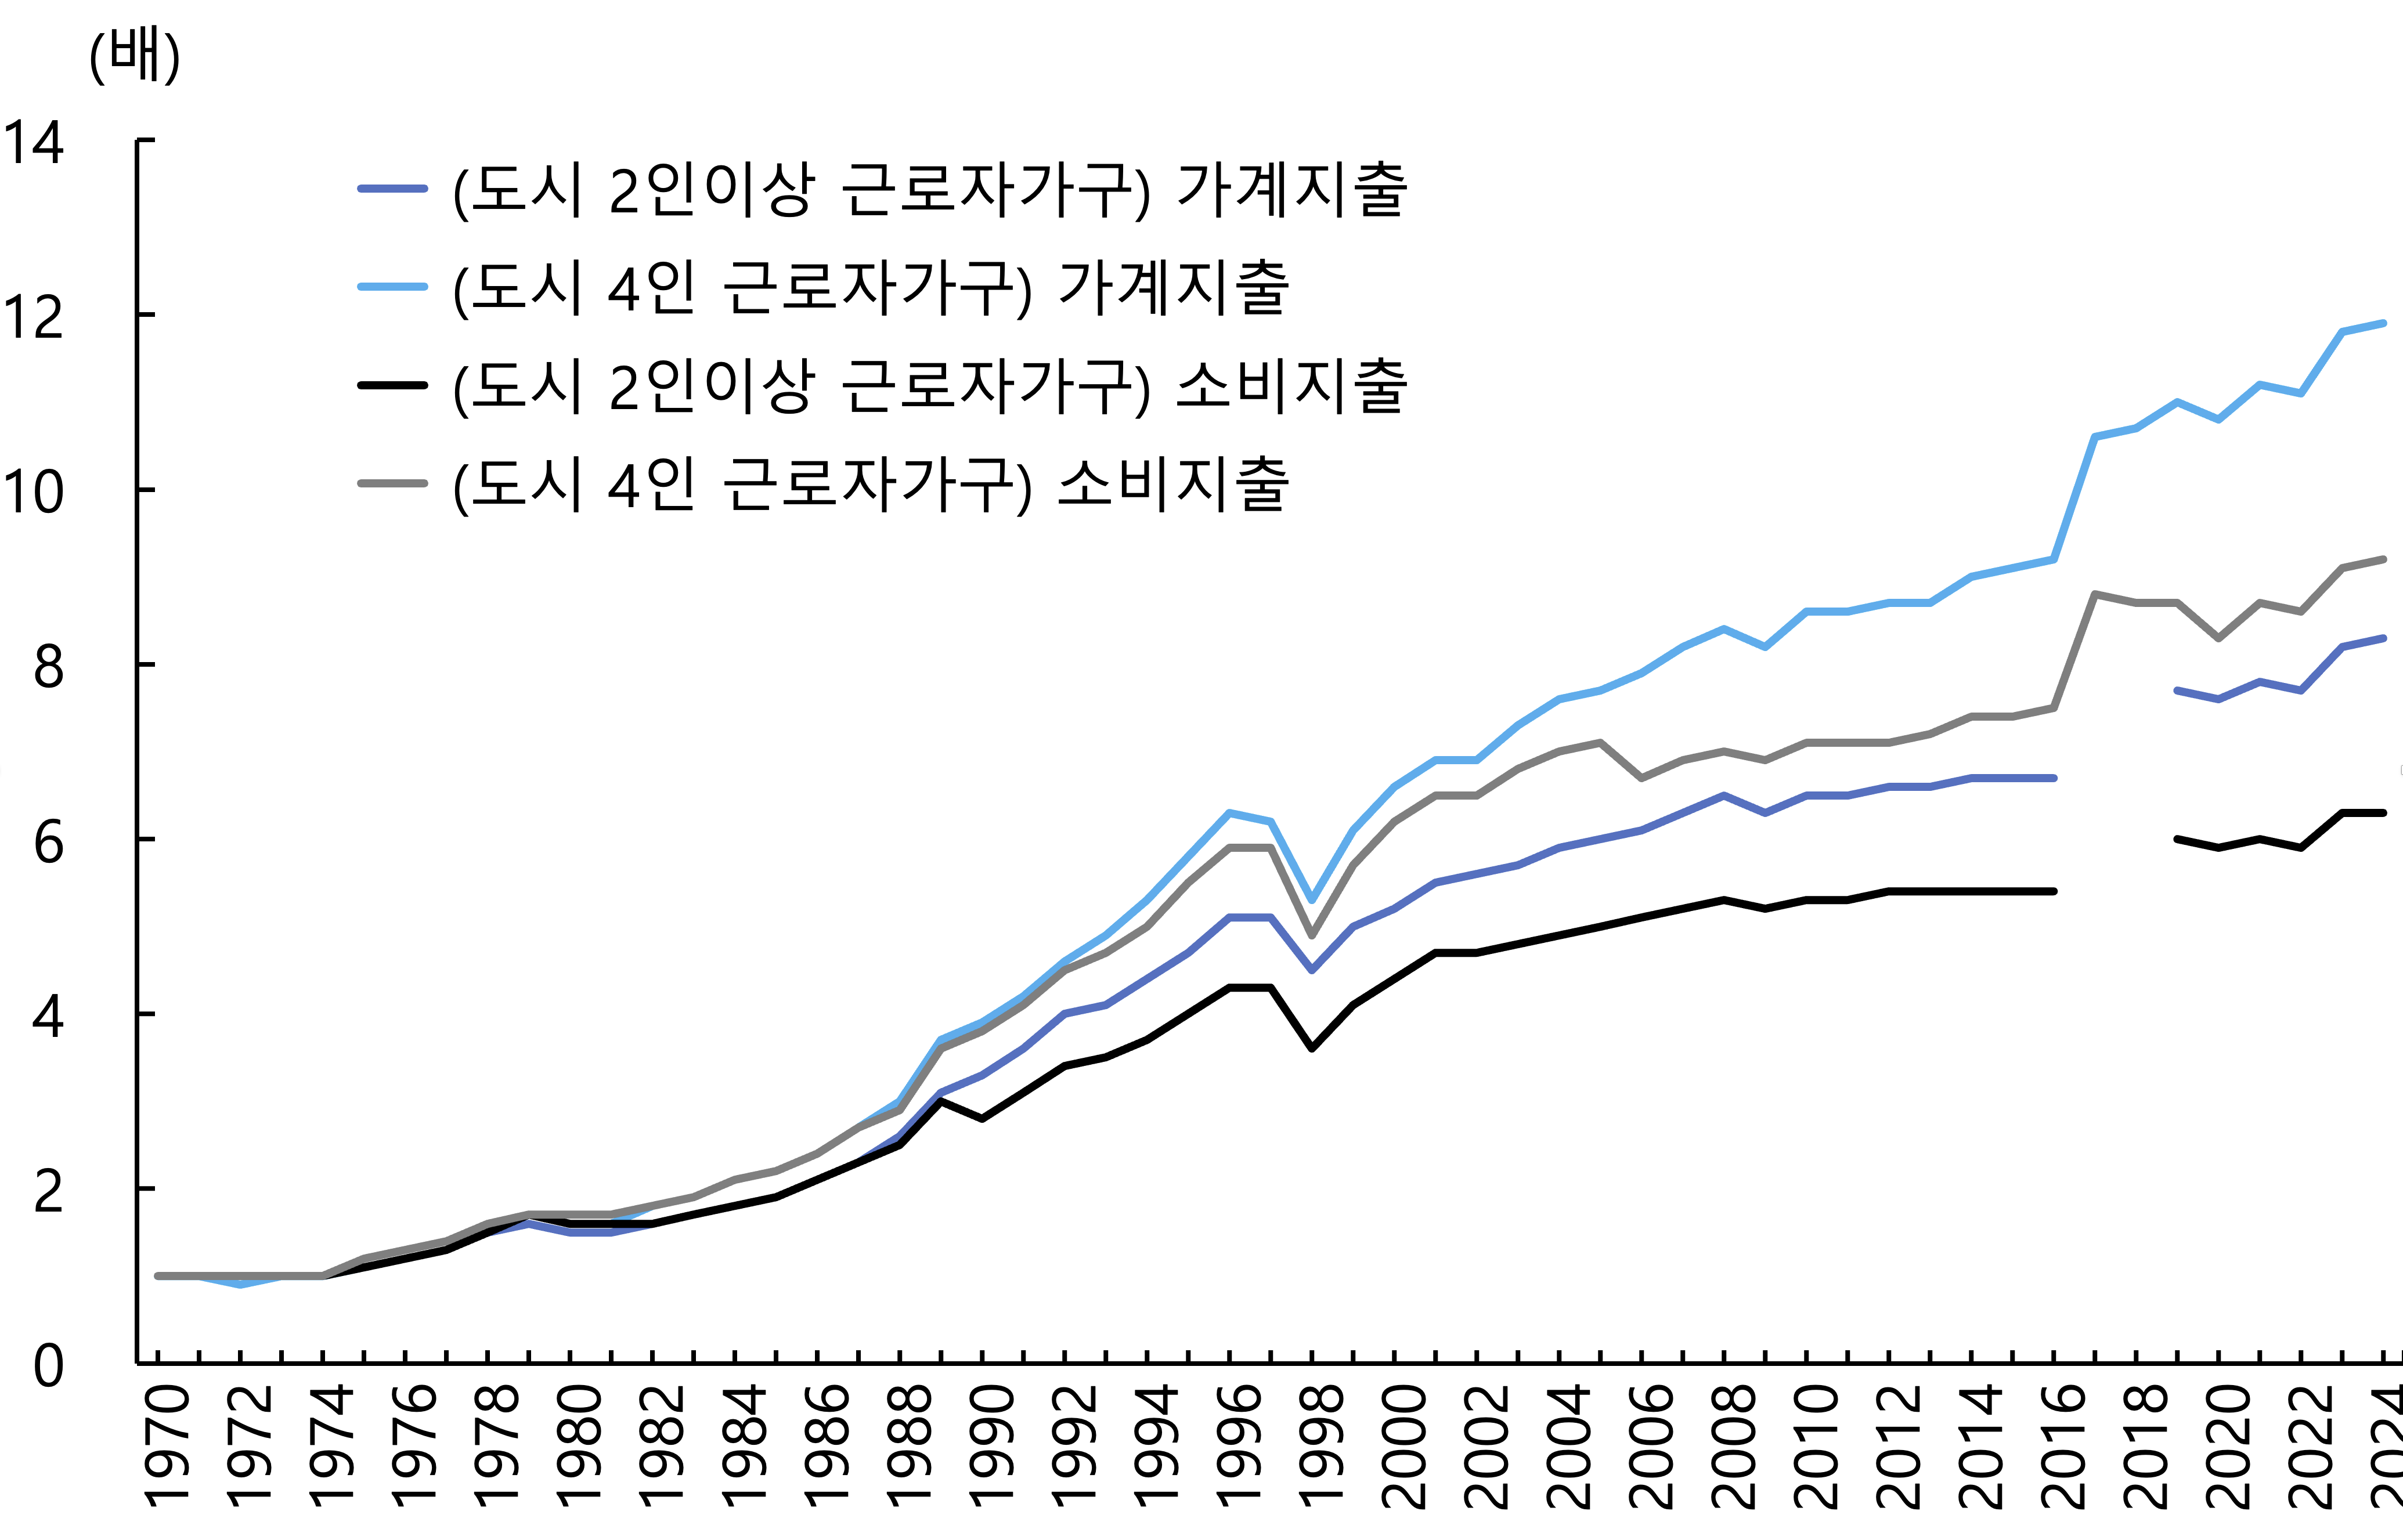
\includegraphics[width=.5\textwidth]{pic/fig_ineq_05.png}
    \end{figure}
    \begin{itemize}
        \item 산업화와 민주화, 88서울올림픽, 해외여행 자유화 등을 거치며 가구 지출은 8배 이상 증가하며 소비사회로 진입했다.
    \end{itemize}
\end{frame}

\subsection{분배}
\begin{frame}[<+->]
\frametitle{외환위기 이후 빈곤율이 급등했다.}
    \begin{figure}
        \centering
        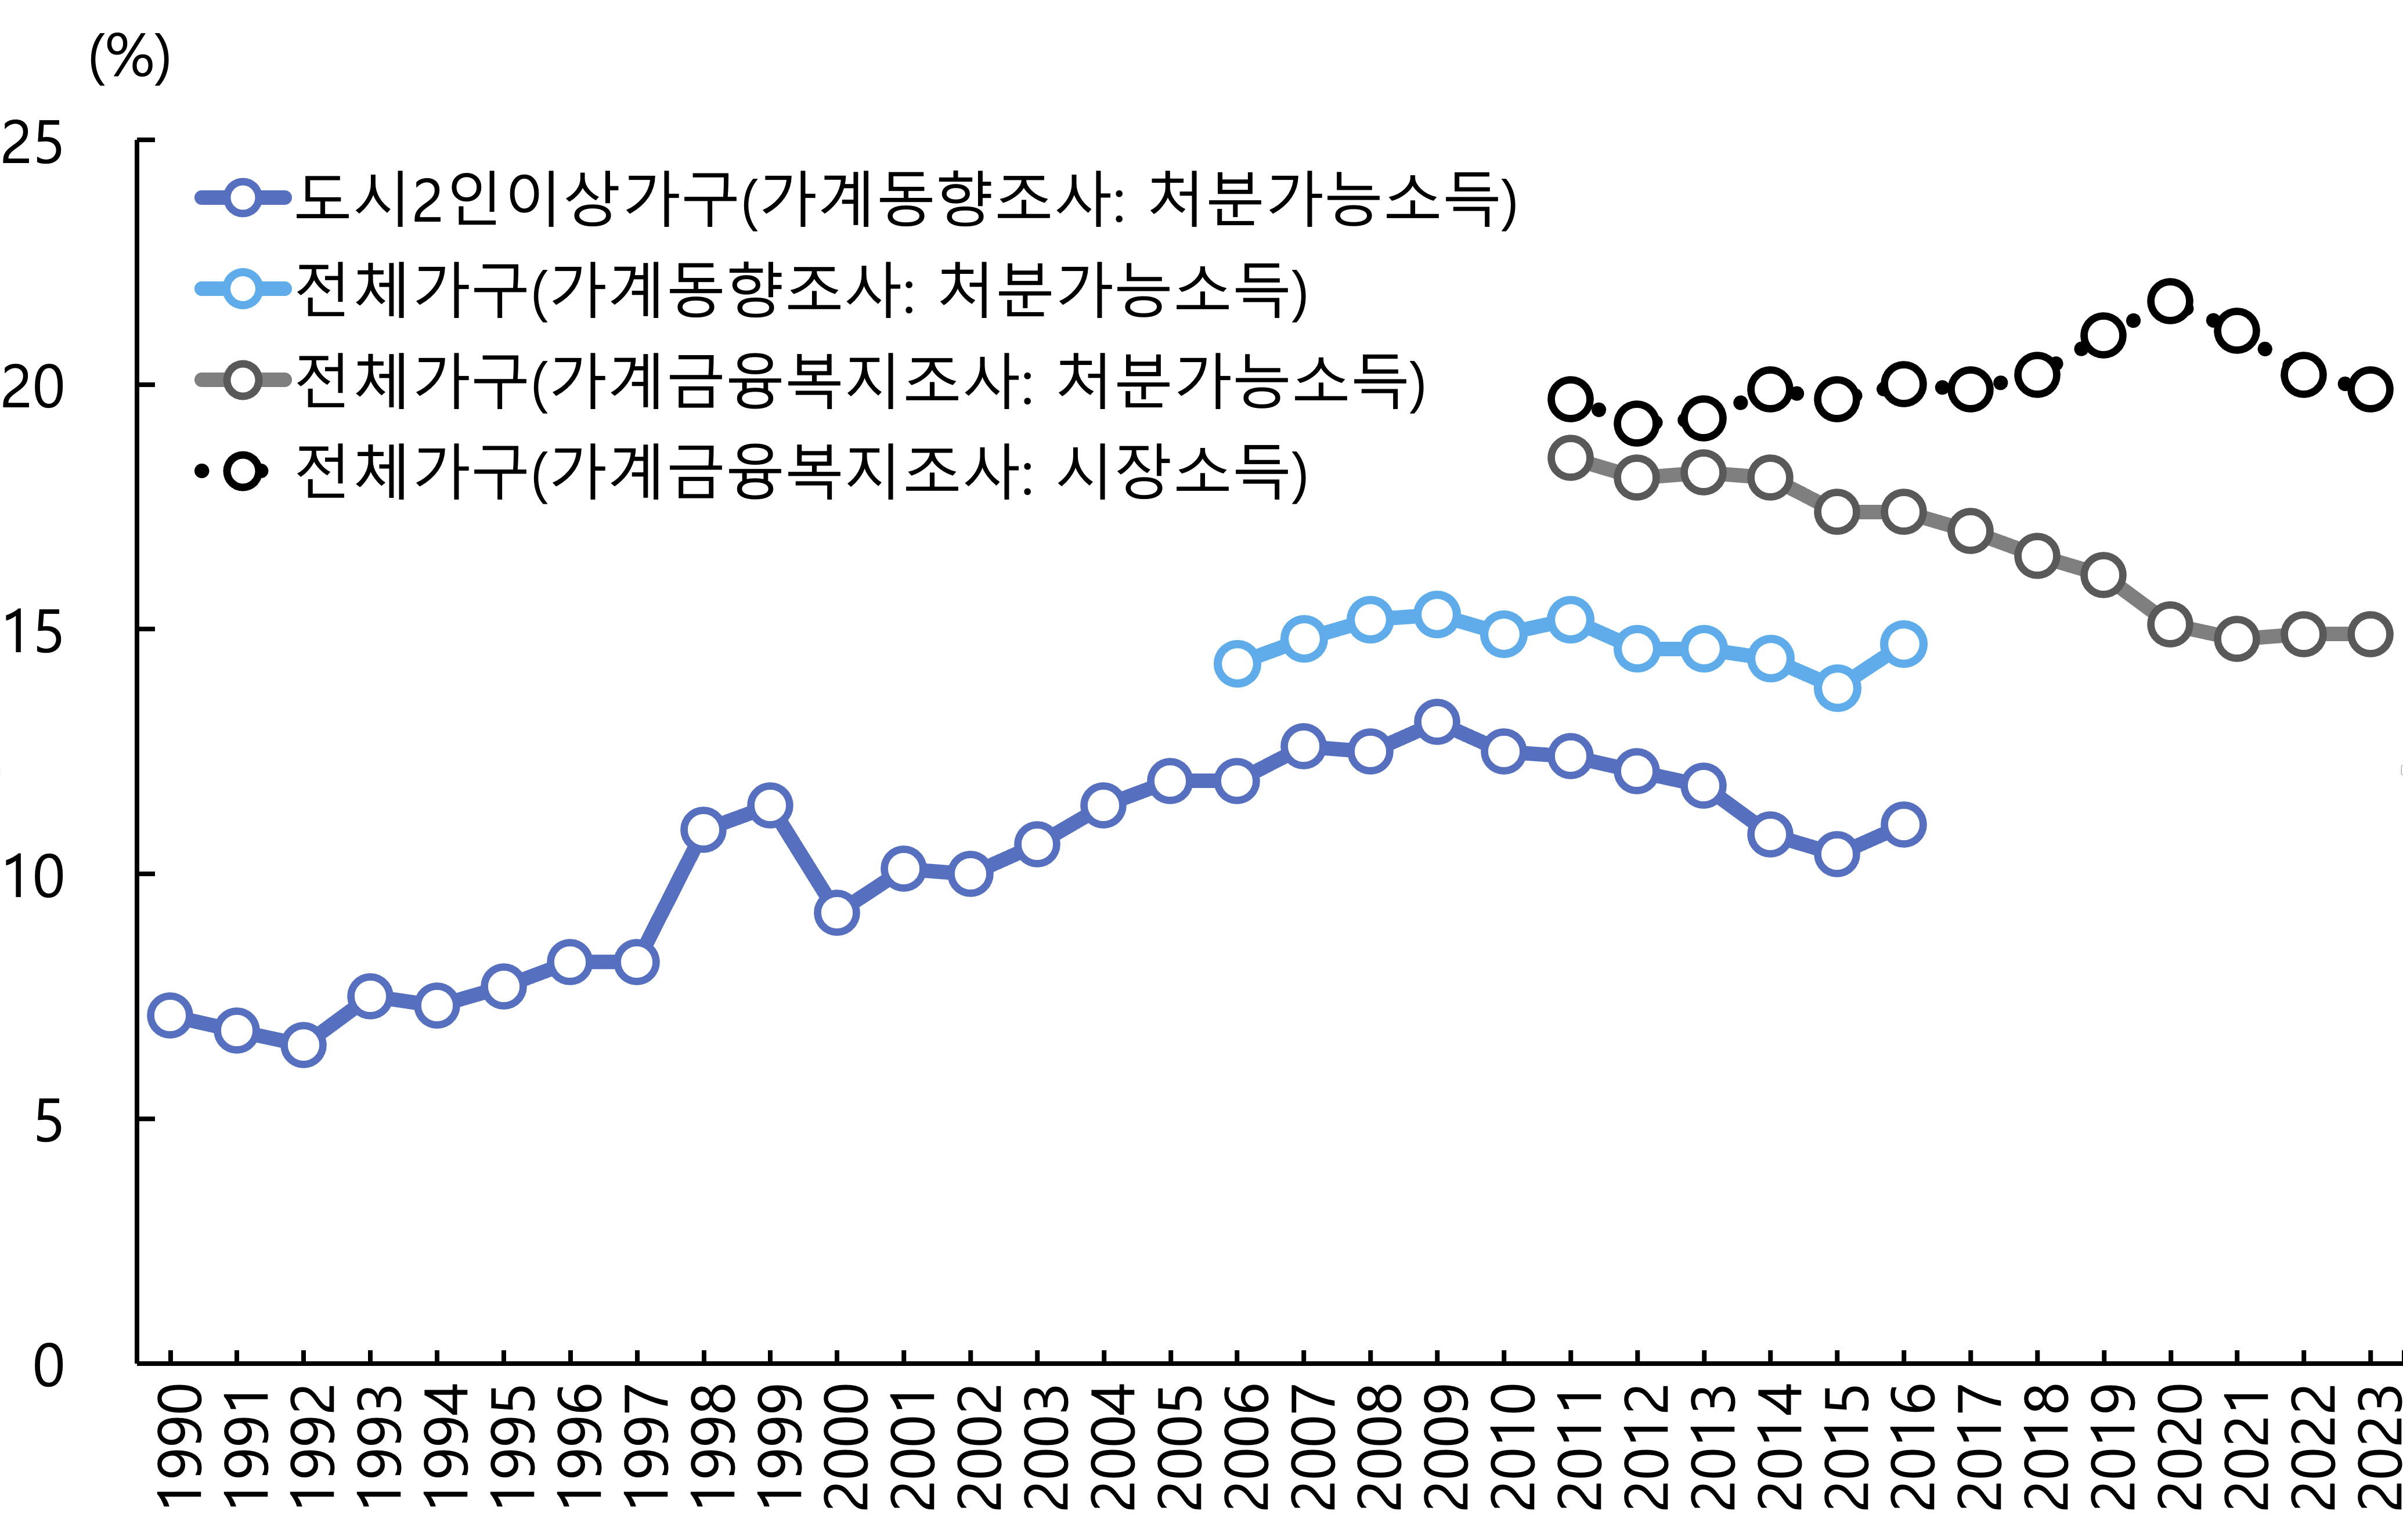
\includegraphics[width=.5\textwidth]{pic/fig_ineq_07.png}
    \end{figure}
    \begin{itemize}
        \item 2010년대까지 (상대)빈곤율ㅊ은 증가 추세였다. 이후 조세와 공적이전소득의 재분배 효과에 의해 빈곤율은 하락하였다.
    \end{itemize}
\end{frame}

\begin{frame}[<+->]
\frametitle{불평등 역시 빈곤율과 유사한 양상을 띈다.}
    \begin{figure}
        \centering
        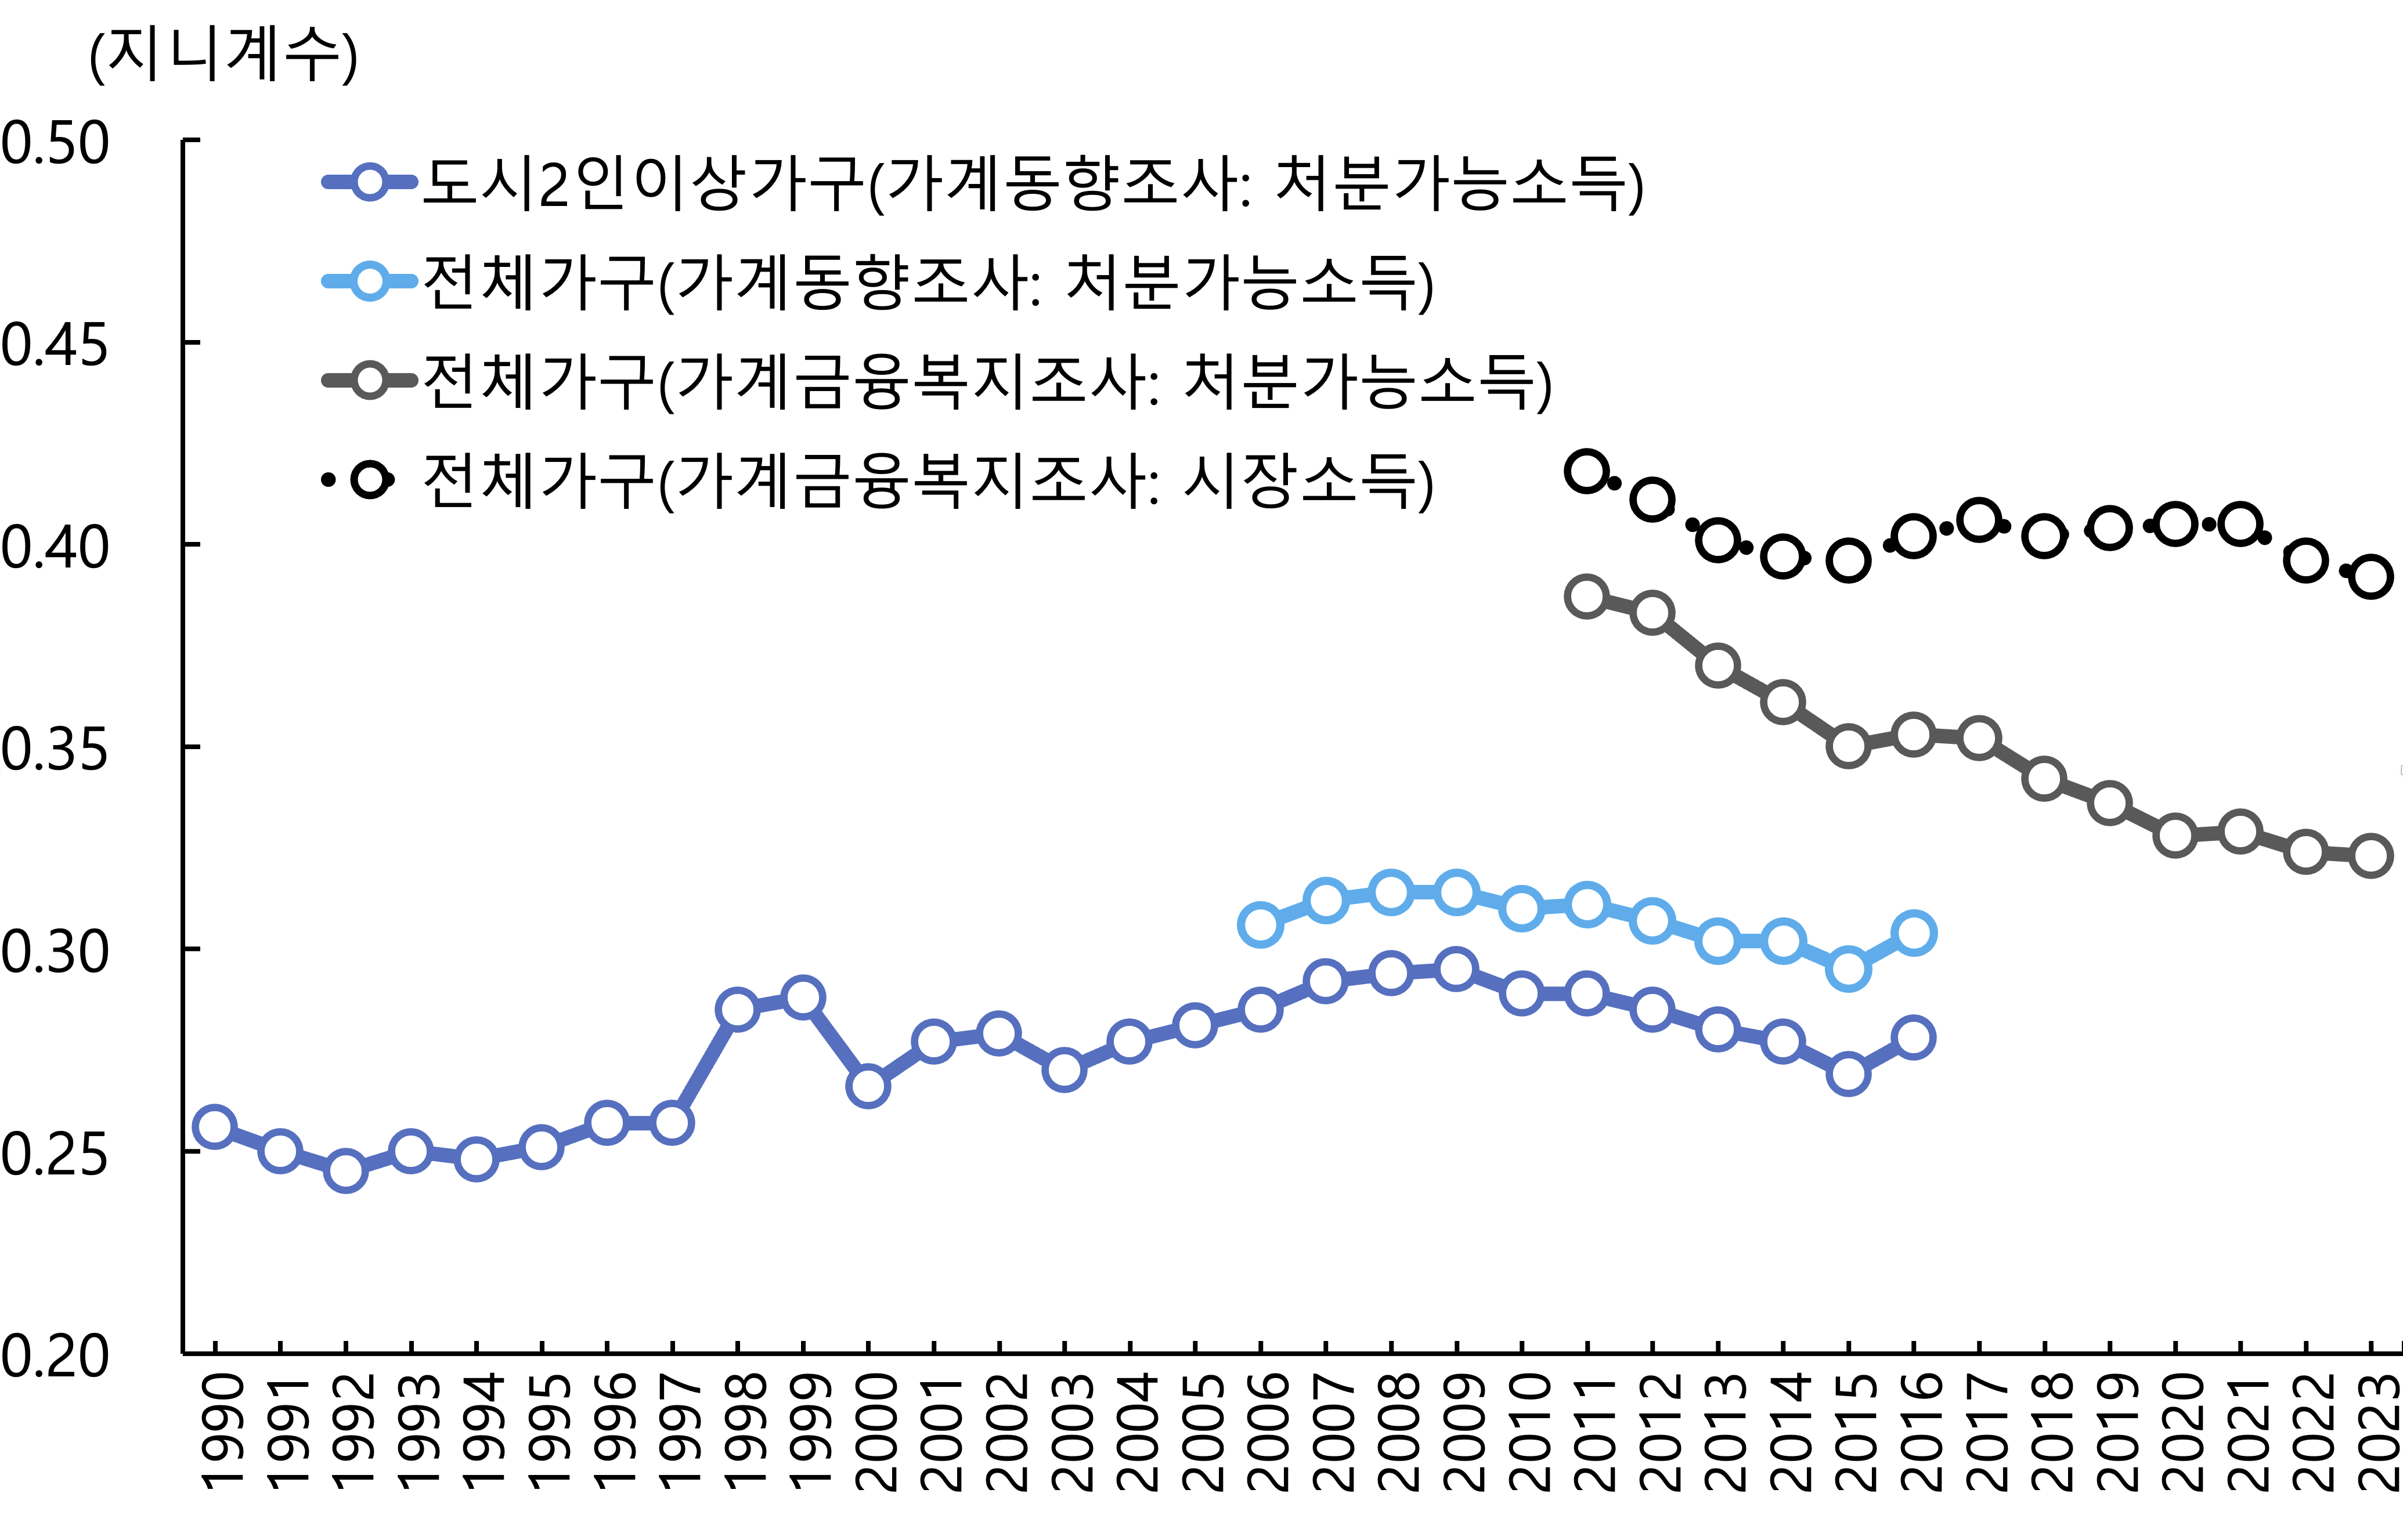
\includegraphics[width=.5\textwidth]{pic/fig_ineq_08.png}
    \end{figure}
    \begin{itemize}
        \item 지니계수는 외환위기와 2000년대에 상승하였지만, 2010년대 복지 확대로 처분가능소득 기준의 불평등은 완화되었다.
    \end{itemize}
\end{frame}

\begin{frame}[<+->]
\frametitle{소득의 양극화가 뚜렷해졌다가 완화되었다.}
    \begin{figure}
        \centering
        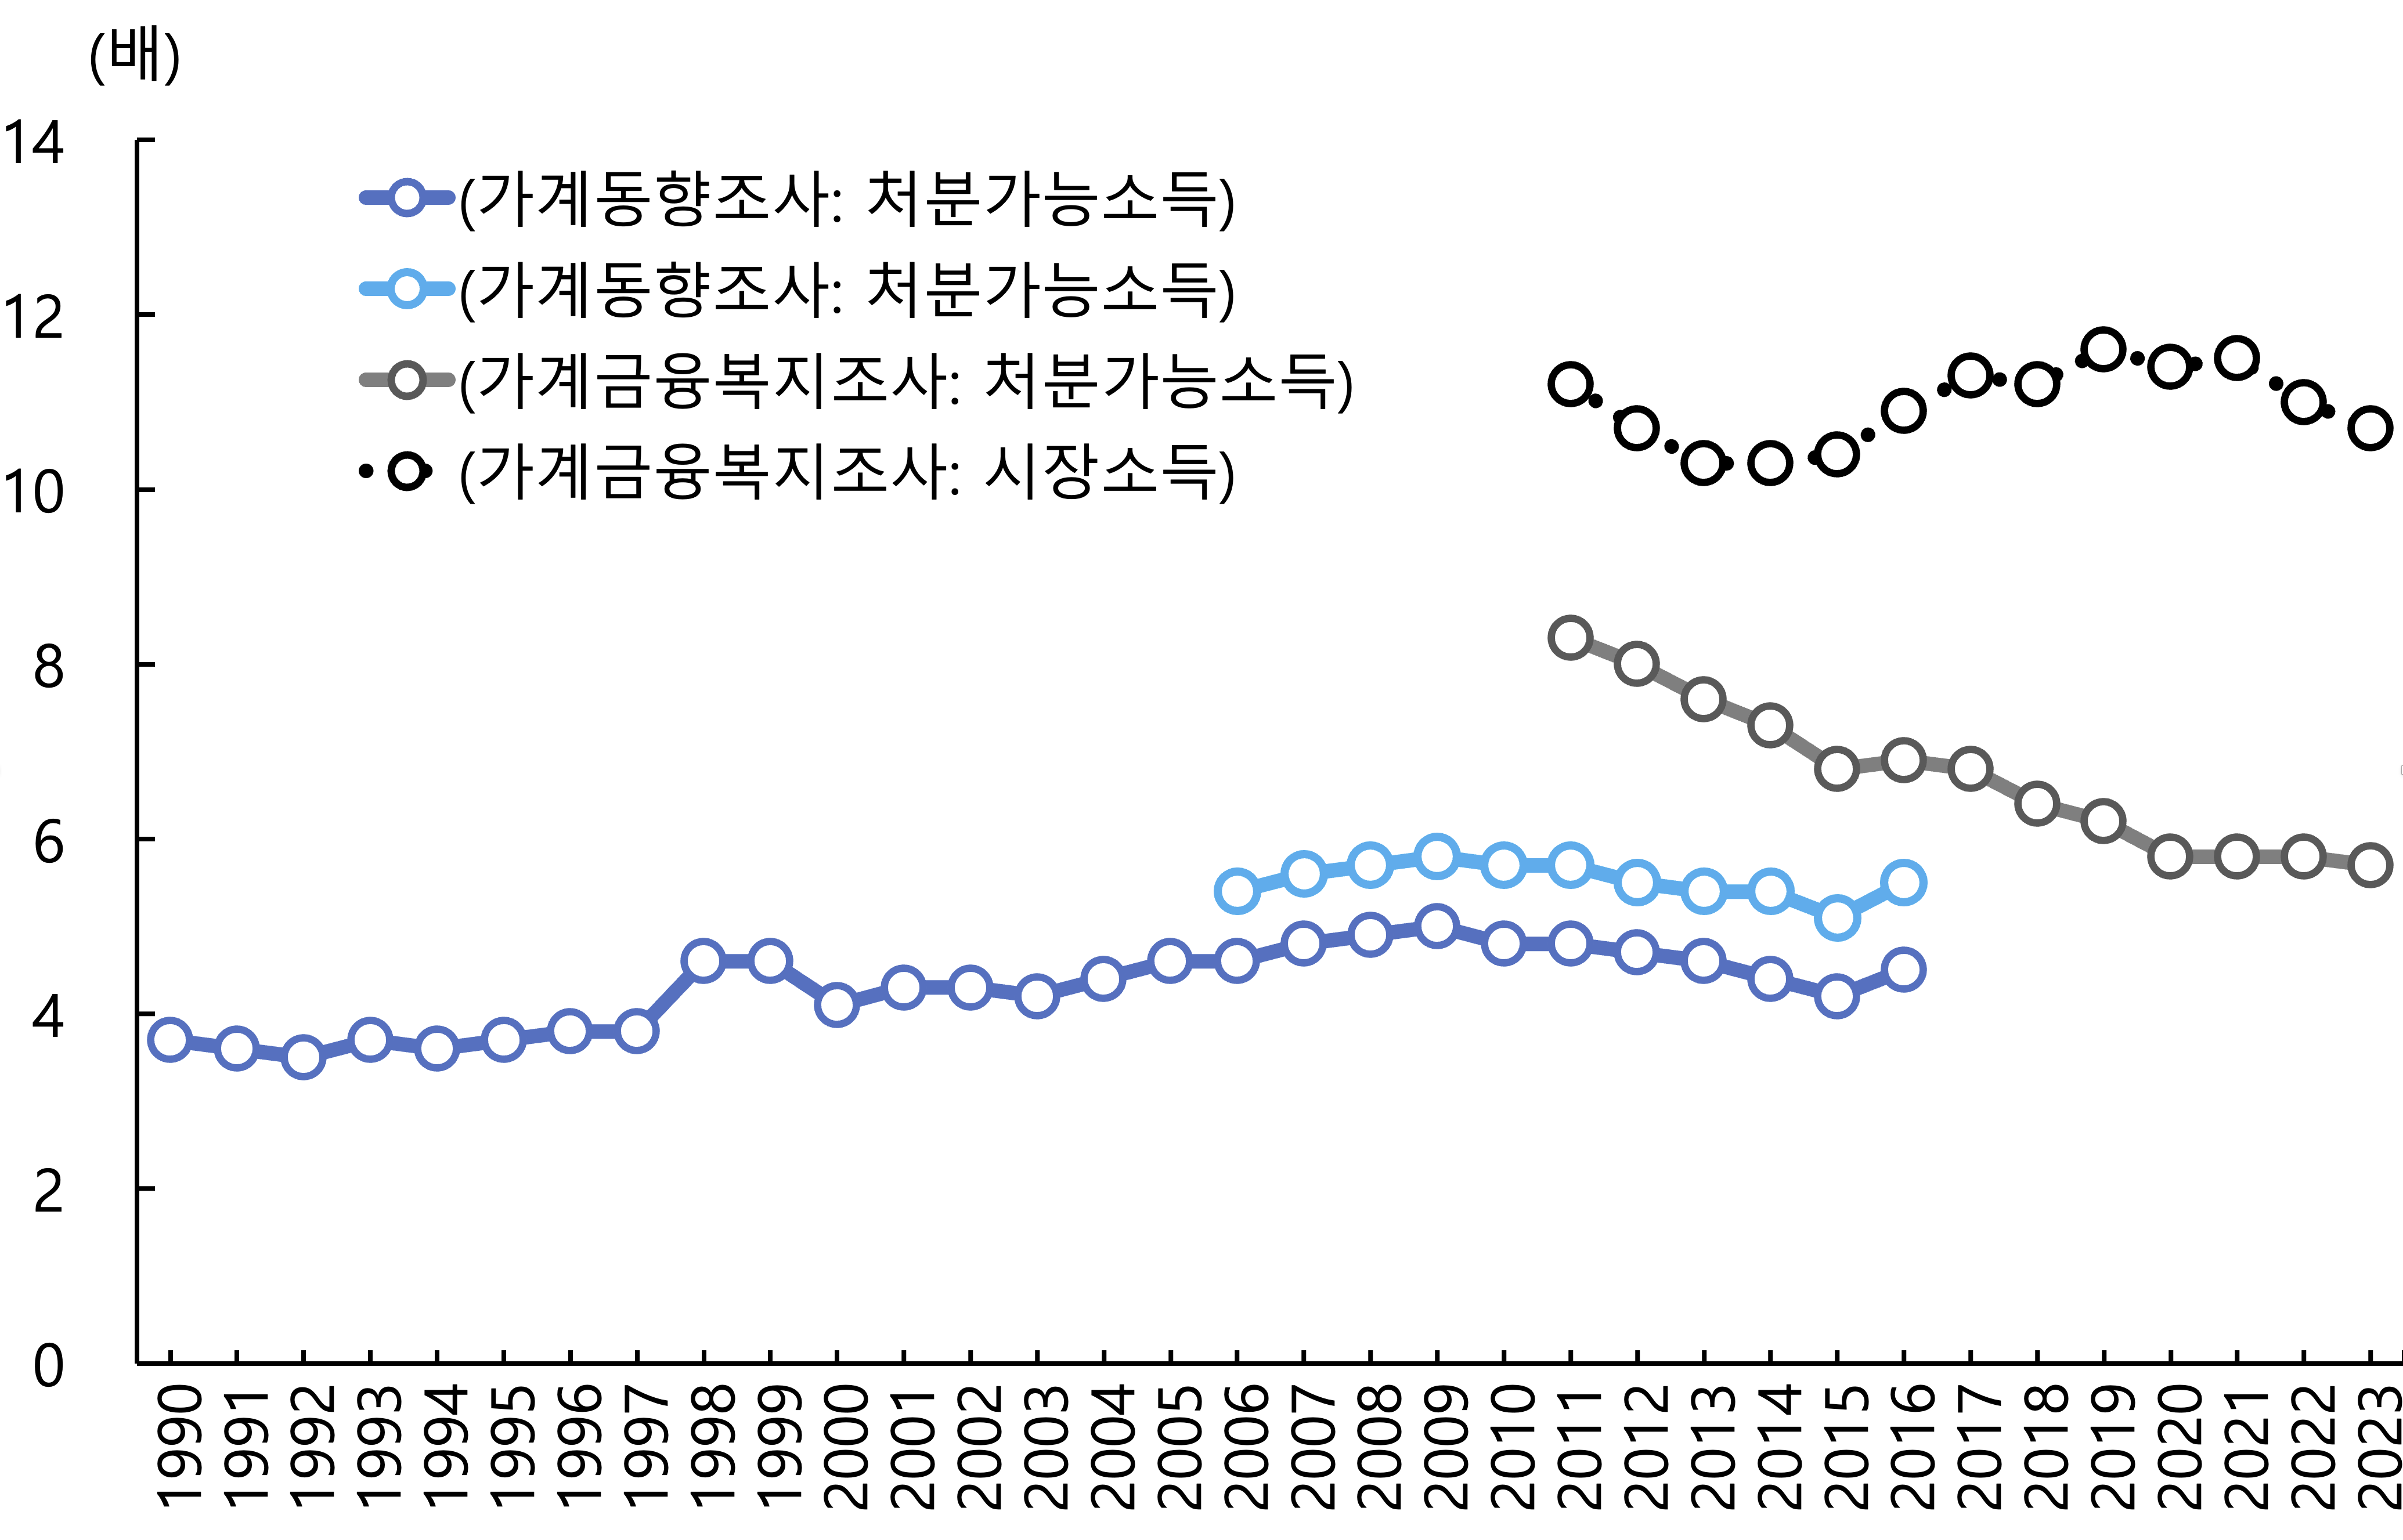
\includegraphics[width=.5\textwidth]{pic/fig_ineq_09.png}
    \end{figure}
    \begin{itemize}
        \item 상·하위 20\% 소득 격차 역시 점진적으로 증가 추세였으나, 최근들어 점차 줄어들고 있다.
    \end{itemize}
\end{frame}

\begin{frame}[<+->]
\frametitle{복지지출이 급증하며 복지국가의 길을 열었다.}
    \begin{figure}
        \centering
        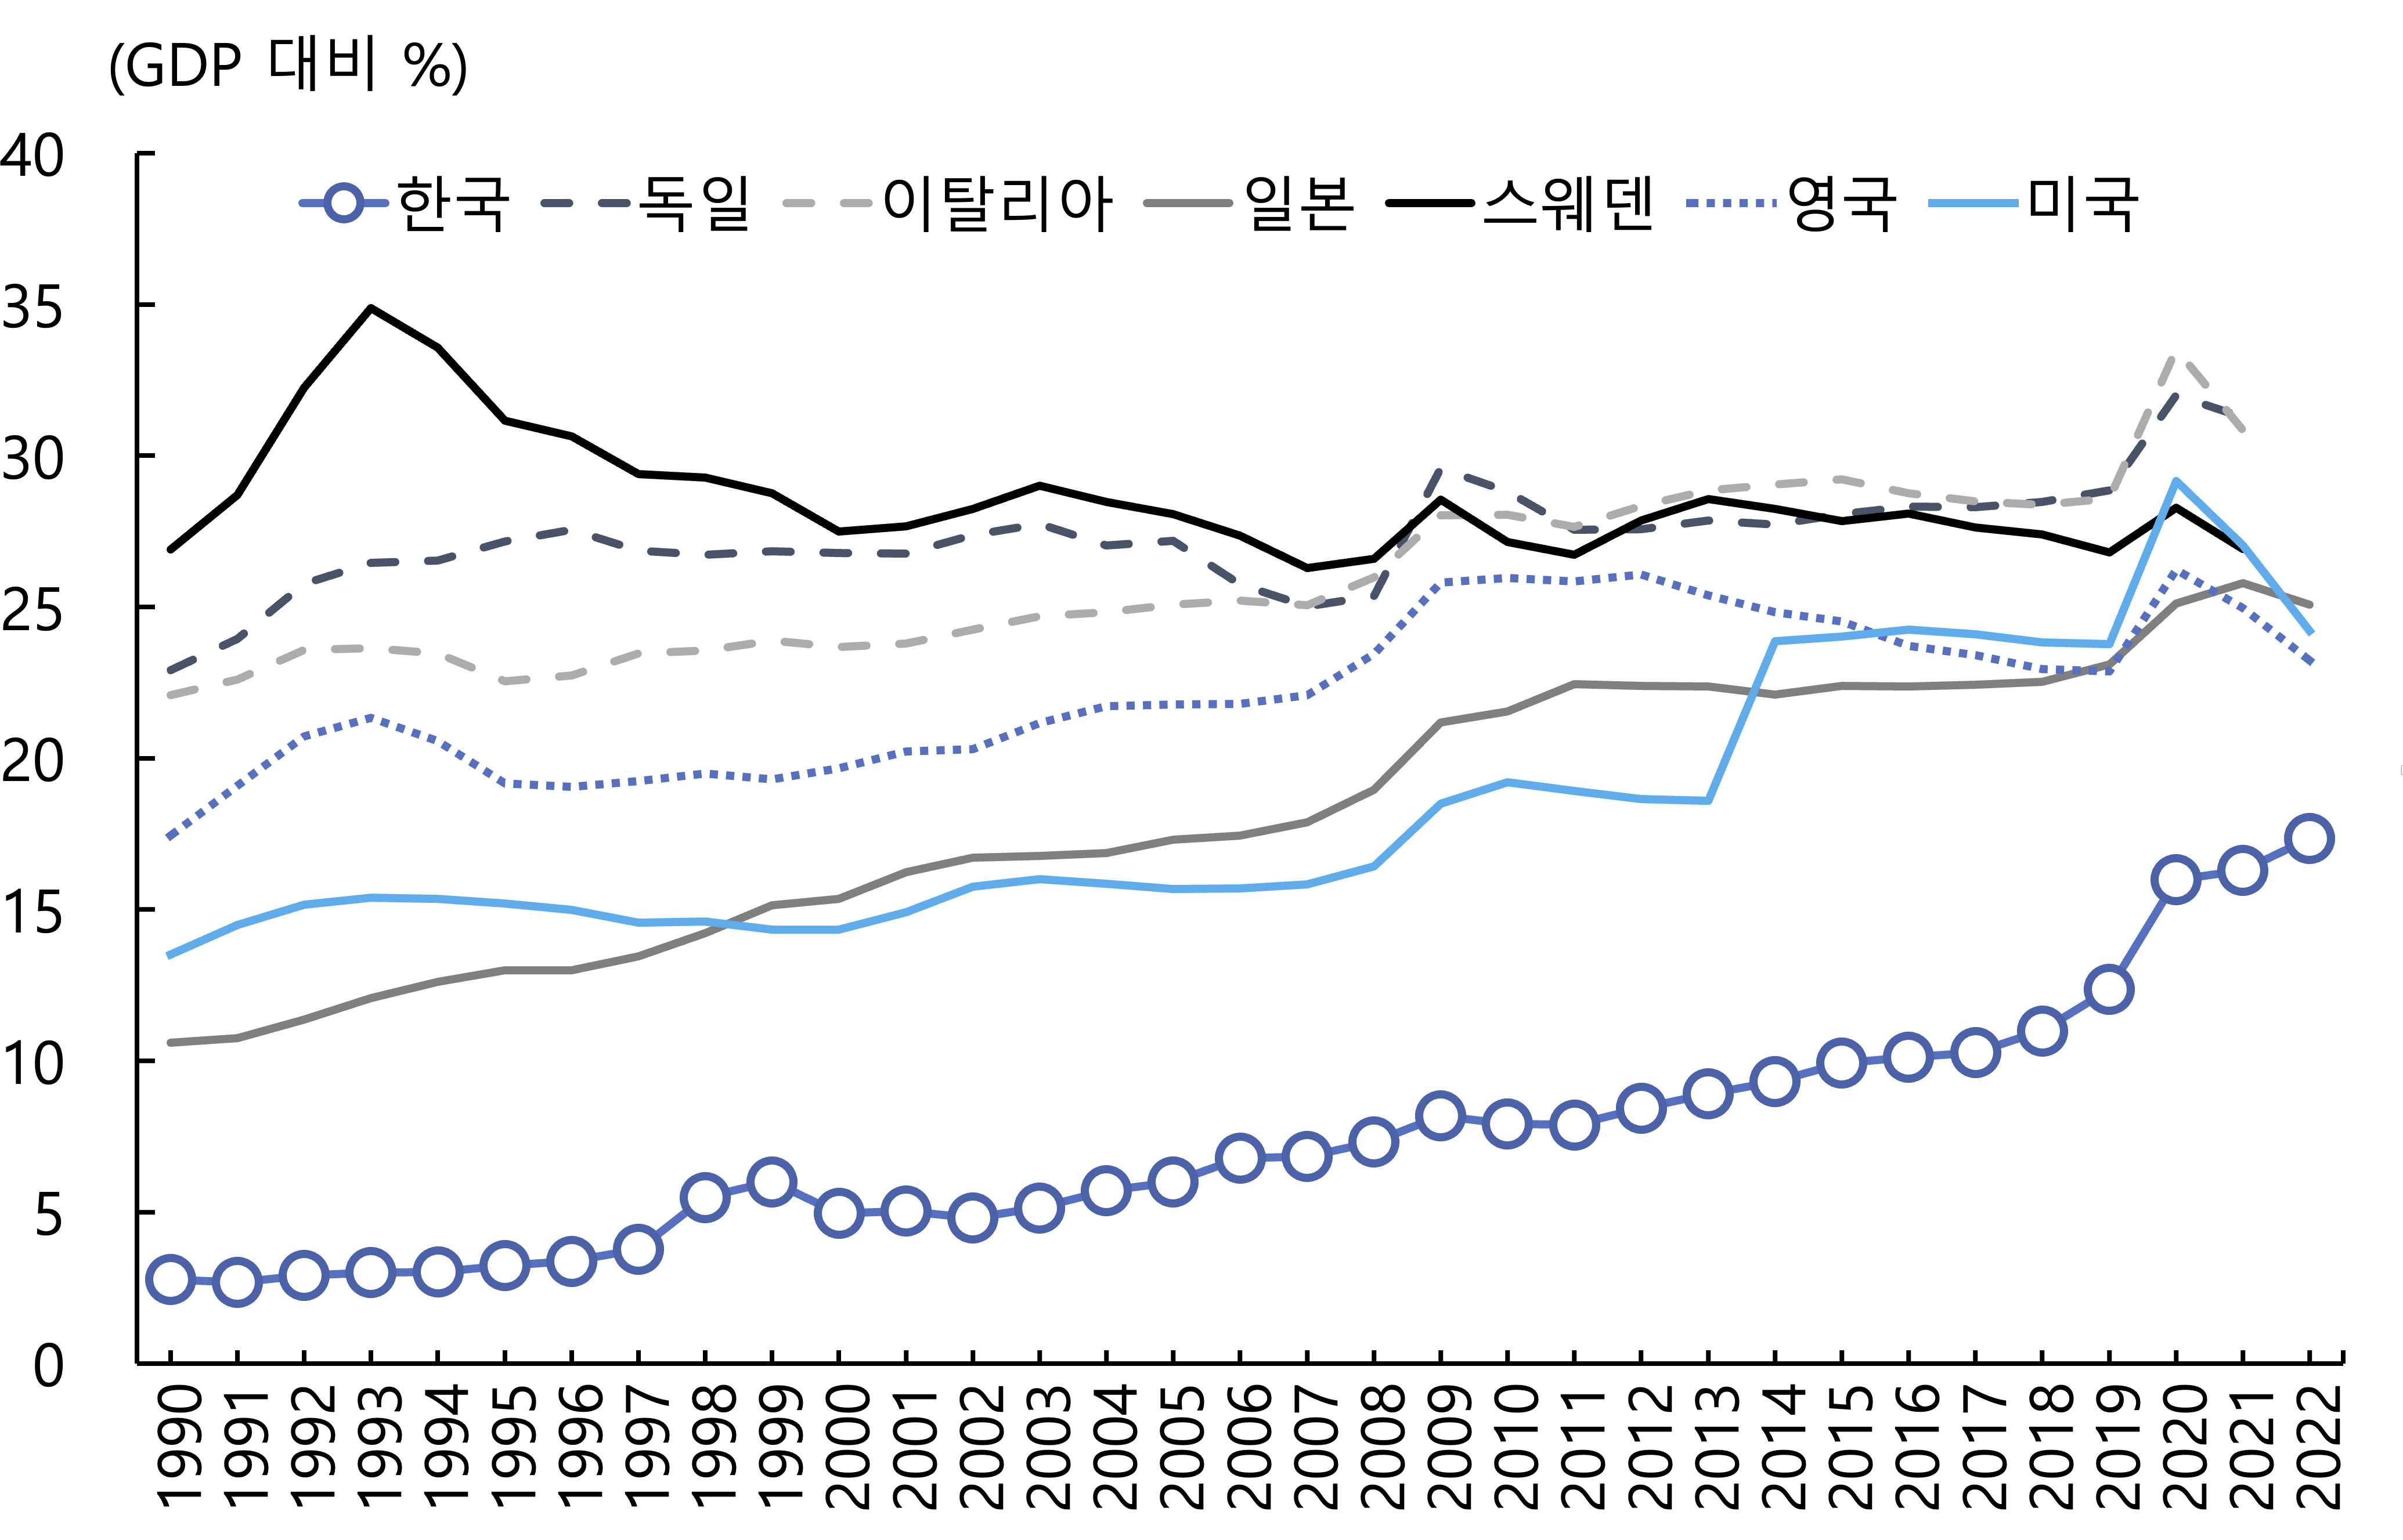
\includegraphics[width=.5\textwidth]{pic/fig_ineq_10.png}
    \end{figure}
    \begin{itemize}
        \item GDP 대비 사회복지지출은 2000년 5.0\% 수준에서 2022년 17.4\%로, 주요 국가들과의 격차를 빠르게 좁히고 있다.
    \end{itemize}
\end{frame}

\begin{frame}[<+->]
\frametitle{공적 이전소득이 취약계층의 삶을 지탱했다.}
    \begin{figure}
        \centering
        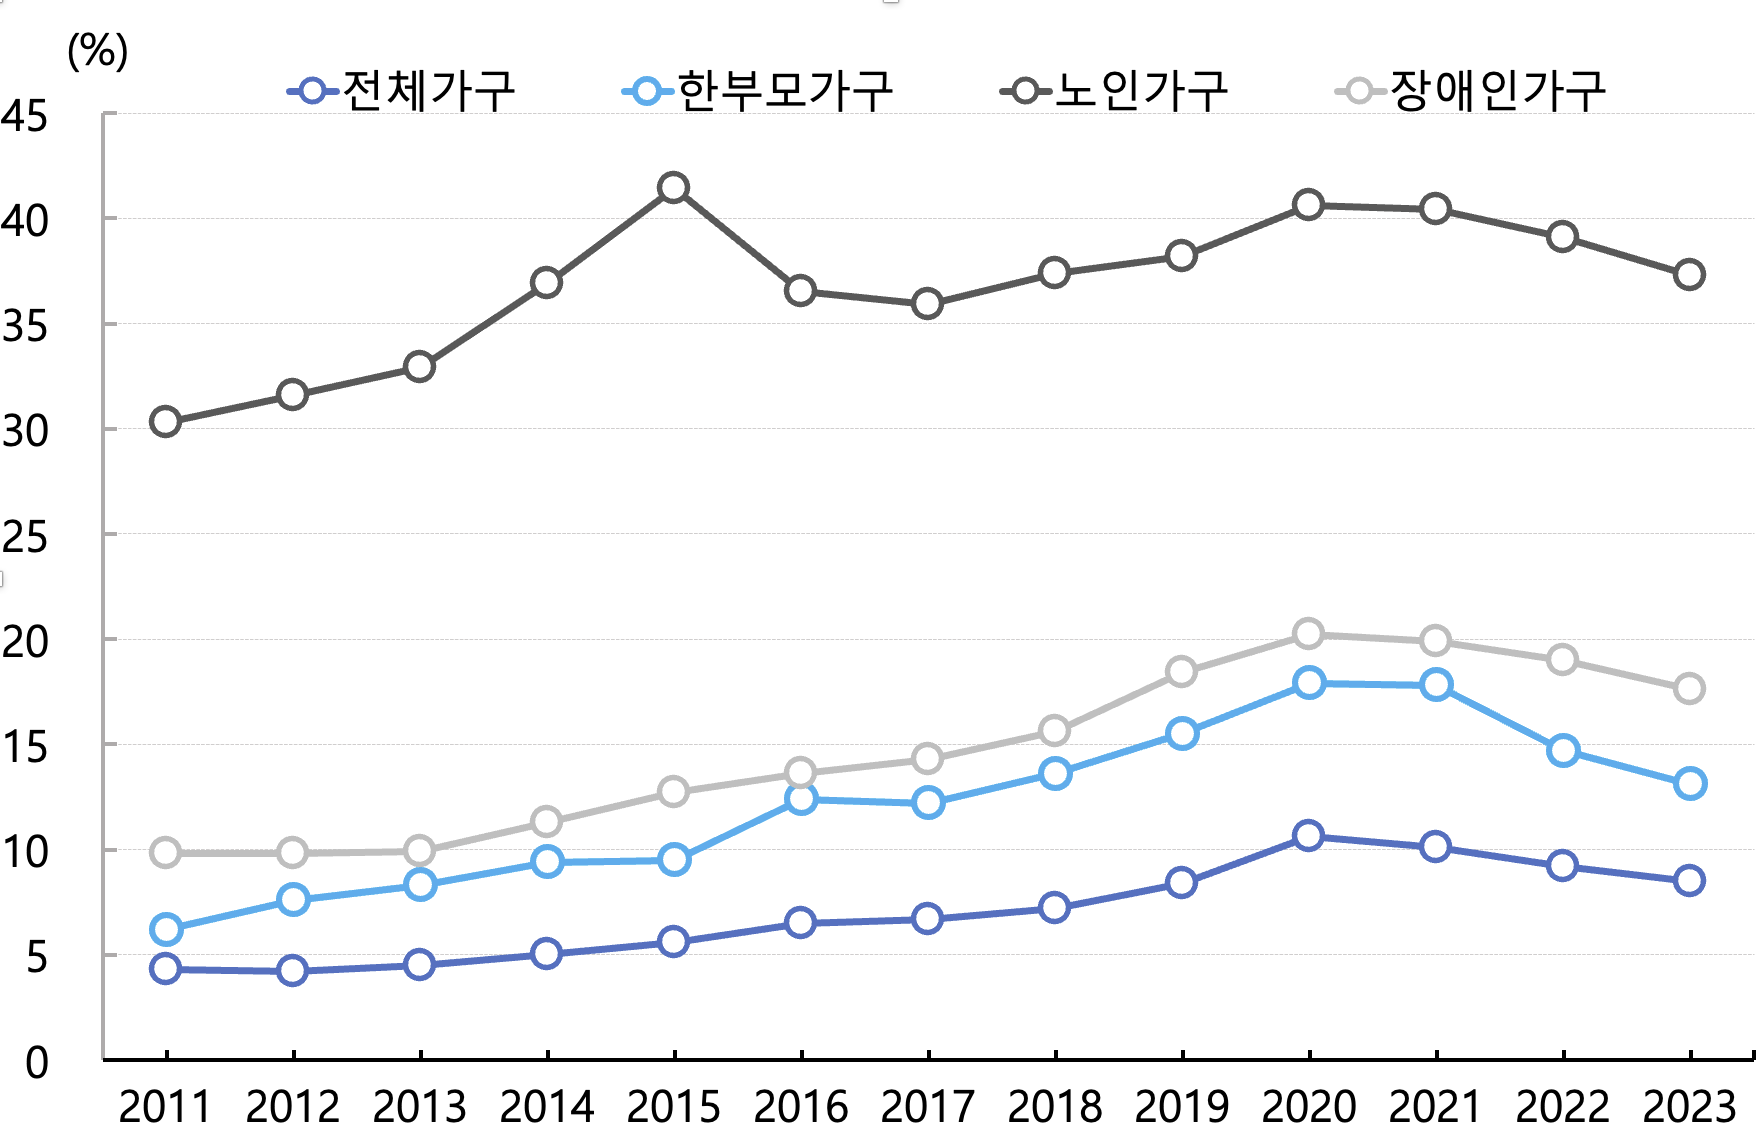
\includegraphics[width=.5\textwidth]{pic/fig_ineq_11.png}
    \end{figure}
    \begin{itemize}
        \item 노인·장애인·한부모 가구의 소득에서 공적 이전소득 비중이 두 자릿수까지 확대되며, 복지국가 전환을 보여주었다.
    \end{itemize}
\end{frame}


\section{맺는말}%
\begin{frame}[<+->]
\frametitle{한국경제의 지난 80년}
    \begin{itemize}
        \item 한국경제가 80년간 이룬 성취는 동시기 전세계 최고수준이라 할 수 있다.
            \begin{itemize}[<+->]
                \item 전후 폐허 속에서 세계 10위권의 경제규모를 달성.
                \item 국민경제의 수준 역시 선진국에 진입.
                \item 수차례 경제위기에도 놀라운 회복력을 보임.
            \end{itemize}
        \item 다만 당면한 근본적 문제는 과거와 같은 긍정적 미래를 보장하지 않는다.
            \begin{itemize}[<+->]
                \item 저성장 고착화 및 불투명한 신성장 동력.
                \item 인구구조 및 복지제도 확대에 따른 복지부담 증가 및 재원 마련.
                \item 불평등에 대한 지표와 인식간의 괴리.
            \end{itemize}
    \end{itemize}
\end{frame}
%------------------------------------------------
\end{document}
%------------------------------------------------
